\chapter{Solving the Stokes equations with the FEM} \label{solvingFEM} %%%%%%%%%%%%%%%%%%%%%%%%%%%%%%
\begin{flushright} {\tiny {\color{gray} chapter\_fem2.tex}} \end{flushright}

\section{A quick tour of similar literature} 

\begin{itemize} 
\item {\it Treatise on Geophysics}, Volume 7, Edited by D. Bercovici and G. Schubert: 
"Numerical Methods for Mantle Convection", by S.J. Zhong, D.A. Yuen, L.N. Moresi and M.G. Knepley. Note that it is a revision of the previous edition chapter by S.J. Zhong, D.A. Yuen and L.N. Moresi, Volume 7, pp. 227-252, 2007.

\item {\it Computational Science I}, Lecture Notes for CAAM 519, M.G. Knepley, 2017.
\url{https://cse.buffalo.edu/~knepley/classes/caam519/}

\item {\it Numerical Modeling of Earth Systems - An introduction to computational methods with focus onsolid Earth applications of continuum mechanics}, Th.W. Becker and B.J.P. Kaus, 2018.
\url{http://www-udc.ig.utexas.edu/external/becker/Geodynamics557.pdf}

\item {\it Myths and Methods in Modeling}, M. Spiegelman, 2000.
\url{https://earth.usc.edu/~becker/teaching/557/reading/spiegelman_mmm.pdf}

\end{itemize}
 
%6.3 of donea and huerta

In the case of an incompressible flow, we have seen that the continuity (mass conservation)
equation takes the simple form ${\bm \nabla}\cdot{\bm v}=0$. In other word flow takes place 
under the constraint that the divergence of its velocity field is exactly zero eveywhere 
(solenoidal constraint), i.e. it is divergence free. \index{divergence free}

We see that the pressure in the momentum equation is then a degree of freedom which is needed 
to satisfy the incompressibilty constraint (and it is not related to any constitutive equation)
\cite{dohu}. In other words the pressure is acting as a Lagrange multiplier of the incompressibility
constraint. 

Various approaches have been proposed in the literature to deal with the 
incompressibility constraint but we will only focus on the penalty method 
(section \ref{sec_penalty}) and the so-called mixed finite element method
\ref{sec_mixed}.
 %---------------------------------------------------------------------------

\newpage %%%%%%%%%%%%%%%%%%%%%%%%%%%%%%%%%%%%%%%%%%%%%%%%%%%%%%%%%%%%%%%%%%%%%%%%%%%%%%%%%%%%%%%%%%
\section{Strong and weak forms} \begin{flushright} {\tiny {\color{gray} \tt strongweak.tex}} \end{flushright}
%------------------------------------------------------------------------------

\index{general}{strong form} 

As we have seen in Section~\ref{sec:diff1D}
the strong form consists of the governing equation and the boundary conditions, i.e. 
the mass, momentum and energy conservation equations supplemented with Dirichlet and/or Neumann
boundary conditions on (parts of) the boundary. Ultimately we have two main unknowns that 
we wish to solve for: velocity (a vector) and pressure (a scalar).

\index{general}{weak form}
To develop the finite element formulation, the partial differential equations 
must be restated in an integral form called the weak form. In essence the PDEs are 
first multiplied by an arbitrary function and integrated over the domain.

 %--------------------------------------------

\newpage %%%%%%%%%%%%%%%%%%%%%%%%%%%%%%%%%%%%%%%%%%%%%%%%%%%%%%%%%%%%%%%%%%%%%%%%%%%%%%%%%%%%%%%%%%
\section{Which velocity-pressure pair for Stokes?}\label{ss:pair}\subsubsection{The bi/tri-linear velocity - constant pressure element ($Q_1\times P_0$)}
\includegraphics[width=3cm]{images/under_construction}

\subsubsection{The bi/tri-quadratic velocity - discontinuous linear pressure element ($Q_2 \times P_{-1}$)}
\includegraphics[width=3cm]{images/under_construction}

\subsubsection{The bi/tri-quadratic velocity - bi/tri-linear pressure element ($Q_2 \times Q_1$)}
\includegraphics[width=3cm]{images/under_construction}

\subsubsection{The stabilised bi/tri-linear velocity -  bi/tri-linear pressure element ($Q_1\times Q_1$-stab)}
\includegraphics[width=3cm]{images/under_construction}

\subsubsection{The MINI triangular element ($P_1^+\times P_1$)}
\includegraphics[width=3cm]{images/under_construction}

\subsubsection{The quadratic velocity - linear pressure triangle ($P_2\times P_1$)}
\includegraphics[width=3cm]{images/under_construction}

\subsubsection{The Crouzeix-Raviart triangle ($P_2^+\times P_{-1}$)}
\includegraphics[width=3cm]{images/under_construction}

\subsection{Other elements}

P1P0

P1P1

Q2Q2

P2P2

 %-----------------

\newpage %%%%%%%%%%%%%%%%%%%%%%%%%%%%%%%%%%%%%%%%%%%%%%%%%%%%%%%%%%%%%%%%%%%%%%%%%%%%%%%%%%%%%%%%%%
\section{The penalty approach for viscous flow}\label{sec:penalty}\begin{flushright} {\tiny {\color{gray} penalty.tex}} \end{flushright}
%~~~~~~~~~~~~~~~~~~~~~~~~~~~~~~~~~~~~~~~~~~~~~~~~~~~~~~~~~~~~~~~~~~~~~~~~~~~~~~~~~~~~~~~~~~~~~~~~~~

\label{sec_penalty}

\index{general}{Penalty Formulation}

In order to impose the incompressibility constraint, two widely used procedures are available, namely the 
Lagrange multiplier method and the penalty method \cite{bathe82,hugh}. The latter is implemented in {\sc elefant}, which allows for the elimination of the pressure variable from the momentum equation (resulting in a reduction of the matrix size).%, based on a relaxation of the incompressibility constraint. 

Mathematical details on the origin and validity of the penalty approach applied to the Stokes problem can for instance be found in  \cite{cuss86}, \cite{redd82} or \cite{gunz89}.

The penalty formulation of the mass conservation equation is based on a relaxation of the incompressibility constraint and writes 
\begin{equation}
{\vec \nabla}\cdot {\vec \upnu} + \frac{p}{\lambda} = 0 \label{penal}
\end{equation}
where $\lambda$ is the penalty parameter, that can be interpreted (and has the same dimension) as a bulk viscosity. It is 
equivalent to say that the material is weakly compressible. It can be shown that if one chooses $\lambda$ to be a 
sufficiently large number, the continuity equation $ {\vec \nabla}\cdot {\vec \upnu} = 0$ will be approximately satisfied in the finite element solution. The value of $\lambda$ is often recommended to be 6 to 7 orders of magnitude larger than the shear viscosity \cite{dohu03,hulb79}.

%Note that Eq. (\ref{penal}) does not form the basis of the penalty method (as often implied) for the Stokes equation but is a consequence of minimising a modified functional of the problem under certain assumptions \cite{redd82}. 

Equation (\ref{penal}) can be used to eliminate the pressure in the momentum equation 
so that the mass and momentum conservation equations fuse to become :
\begin{equation}
{\vec \nabla}\cdot ( 2 \eta \dot\varepsilon({\vec \upnu})) 
+ \lambda {\vec \nabla} ({\vec \nabla }\cdot {\vec \upnu}) = \rho {\bm g} = 0 \label{peneq}
\end{equation}

\cite{mahu78} have established the equivalence for incompressible problems between the reduced integration
of the penalty term and a mixed Finite Element approach if the pressure nodes coincide with the integration points of the reduced rule.

In the end, the elimination of the pressure unknown in the Stokes equations
replaces the original saddle-point Stokes problem \cite{begl05} by an elliptical problem, 
which leads to a symmetric positive definite (SPD) FEM matrix. 
%Such systems always admit a square root triangular matrix (the Cholesky factor, L) and can be solved, once L has been computed (Cholesky factorization), by 2 triangular matrix solves (upper and lower back-substitutions). 
This is the major benefit of the penalized approach 
over the full indefinite solver with the velocity-pressure variables. Indeed, the SPD character of the matrix lends itself 
to efficient solving stragegies and is less memory-demanding since it is sufficient to store only the upper half of the matrix including the diagonal
\cite{gova}
.
\improvement{list codes which use this approach}

%The stress tensor ${\bm \sigma}$ is symmetric ({\it i.e.} $\sigma_{ij}=\sigma_{ji}$). For simplicity
%I will now focus on a Stokes flow in two dimensions. 

Since the penalty formulation is only valid for incompressible flows, then 
$\dot{\bm \epsilon}=\dot{\bm \epsilon}^d$ so that the $d$ superscript is ommitted in what follows.
Because the stress tensor is symmetric one can also rewrite it the following vector format:
\begin{eqnarray}
\left(
\begin{array}{c}
\sigma_{xx}\\
\sigma_{yy}\\
\sigma_{zz}\\
\sigma_{xy}\\
\sigma_{xz}\\
\sigma_{yz}
\end{array}
\right)
&=&
\left(
\begin{array}{c}
-p\\
-p\\
-p\\
0\\
0\\
0
\end{array}
\right)
+2 \eta
\left(
\begin{array}{c}
\dot{\epsilon}_{xx}\\
\dot{\epsilon}_{yy}\\
\dot{\epsilon}_{zz}\\
\dot{\epsilon}_{xy}\\
\dot{\epsilon}_{xz}\\
\dot{\epsilon}_{yz}
\end{array}
\right)
\nonumber\\
&=&
\lambda
\left(
\begin{array}{c}
\dot{\epsilon}_{xx} + \dot{\epsilon}_{yy} + \dot{\epsilon}_{zz}\\
\dot{\epsilon}_{xx} + \dot{\epsilon}_{yy} + \dot{\epsilon}_{zz}\\
\dot{\epsilon}_{xx} + \dot{\epsilon}_{yy} + \dot{\epsilon}_{zz}\\
0 \\ 0 \\ 0
\end{array}
\right)
+2 \eta
\left(
\begin{array}{c}
\dot{\epsilon}_{xx}\\
\dot{\epsilon}_{yy}\\
\dot{\epsilon}_{zz}\\
\dot{\epsilon}_{xy}\\
\dot{\epsilon}_{xz}\\
\dot{\epsilon}_{yz}
\end{array}
\right)\nonumber\\
&=&
\left[
\lambda
\underbrace{
\left(
\begin{array}{cccccc}
1 & 1 & 1 & 0 & 0 & 0 \\
1 & 1 & 1 & 0 & 0 & 0 \\
1 & 1 & 1 & 0 & 0 & 0 \\
0 & 0 & 0 & 0 & 0 & 0 \\
0 & 0 & 0 & 0 & 0 & 0 \\
0 & 0 & 0 & 0 & 0 & 0 
\end{array}
\right)}_{\bm K}
+ \eta
\underbrace{
\left(
\begin{array}{cccccc}
2 & 0 & 0 & 0 & 0 & 0 \\ 
0 & 2 & 0 & 0 & 0 & 0 \\ 
0 & 0 & 2 & 0 & 0 & 0 \\ 
0 & 0 & 0 & 1 & 0 & 0 \\
0 & 0 & 0 & 0 & 1 & 0 \\
0 & 0 & 0 & 0 & 0 & 1 
\end{array}
\right)
}_{\bm C}
\right]
\cdot
\left(
\begin{array}{c}
\frac{\partial u}{\partial x} \\ \\
\frac{\partial v}{\partial y} \\ \\
\frac{\partial w}{\partial z} \\ \\
\frac{\partial u}{\partial y} + \frac{\partial v}{\partial x} \\ \\
\frac{\partial u}{\partial z} + \frac{\partial w}{\partial x} \\ \\
\frac{\partial v}{\partial z} + \frac{\partial w}{\partial y} 
\end{array}
\right) \nonumber
\end{eqnarray}


Remember that
\[
\frac{\partial u}{\partial x} = \sum_{i=1}^4 \frac{\partial \bN_i}{\partial x}\;  u_i 
\quad\quad
\frac{\partial v}{\partial y} = \sum_{i=1}^4 \frac{\partial \bN_i}{\partial y}\;  v_i 
\quad\quad
\frac{\partial w}{\partial z} = \sum_{i=1}^4 \frac{\partial \bN_i}{\partial z}\;  w_i 
\]
and 
\begin{eqnarray}
\frac{\partial u}{\partial y} +\frac{\partial v}{\partial x} 
&=& \sum_{i=1}^4 \frac{\partial \bN_i}{\partial y}\;  u_i
+ \sum_{i=1}^4 \frac{\partial \bN_i}{\partial x}\;  v_i \nonumber\\
\frac{\partial u}{\partial z} +\frac{\partial w}{\partial x} 
&=& \sum_{i=1}^4 \frac{\partial \bN_i}{\partial z}\;  u_i
+ \sum_{i=1}^4 \frac{\partial \bN_i}{\partial x}\;  w_i \nonumber\\
\frac{\partial v}{\partial z} +\frac{\partial w}{\partial y} 
&=& \sum_{i=1}^4 \frac{\partial \bN_i}{\partial z}\;  v_i
+ \sum_{i=1}^4 \frac{\partial \bN_i}{\partial y}\;  w_i \nonumber
\end{eqnarray}
so that
\[
\left(
\begin{array}{c}
\frac{\partial u}{\partial x} \\ \\
\frac{\partial v}{\partial y} \\ \\
\frac{\partial w}{\partial z} \\ \\
\frac{\partial u}{\partial y} + \frac{\partial v}{\partial x} \\ \\
\frac{\partial u}{\partial z} + \frac{\partial w}{\partial x} \\ \\
\frac{\partial v}{\partial z} + \frac{\partial w}{\partial y} 
\end{array}
\right)
=
\underbrace{
\left(
\begin{array}{ccccccccccccc}
\frac{\partial \bN_1}{\partial x} & 0 & 0 &  
\frac{\partial \bN_2}{\partial x} & 0 & 0 &
\frac{\partial \bN_3}{\partial x} & 0 & 0 & \dots &
\frac{\partial \bN_4}{\partial x} & 0 & 0 \\  \\
0 & \frac{\partial \bN_1}{\partial y} & 0 &
0 & \frac{\partial \bN_2}{\partial y} & 0 &
0 & \frac{\partial \bN_3}{\partial y} & 0 & \dots &
0 & \frac{\partial \bN_4}{\partial y} & 0  \\ \\
0 & 0 & \frac{\partial \bN_1}{\partial z}  &
0 & 0 & \frac{\partial \bN_2}{\partial z}  &
0 & 0 & \frac{\partial \bN_3}{\partial z}  & \dots &
0 & 0 & \frac{\partial \bN_4}{\partial z}   \\ \\
\frac{\partial \bN_1}{\partial y} &  \frac{\partial \bN_1}{\partial x} & 0 &
\frac{\partial \bN_2}{\partial y} &  \frac{\partial \bN_2}{\partial x} & 0 &
\frac{\partial \bN_3}{\partial y} &  \frac{\partial \bN_3}{\partial x} & 0 & \dots &
\frac{\partial \bN_4}{\partial y} &  \frac{\partial \bN_4}{\partial x} & 0 \\ \\ 
\frac{\partial \bN_1}{\partial z} & 0 &\frac{\partial \bN_1}{\partial x}  &
\frac{\partial \bN_2}{\partial z} & 0 &\frac{\partial \bN_2}{\partial x}  &
\frac{\partial \bN_3}{\partial z} & 0 &\frac{\partial \bN_3}{\partial x}  & \dots &
\frac{\partial \bN_4}{\partial z} & 0 &\frac{\partial \bN_4}{\partial x}  \\ \\ 
0 & \frac{\partial \bN_1}{\partial z} &  \frac{\partial \bN_1}{\partial y}  &
0 & \frac{\partial \bN_2}{\partial z} &  \frac{\partial \bN_2}{\partial y}  &
0 & \frac{\partial \bN_3}{\partial z} &  \frac{\partial \bN_3}{\partial y}  & \dots &
0 & \frac{\partial \bN_4}{\partial z} &  \frac{\partial \bN_4}{\partial y} 
\end{array}
\right)
}_{\bm B (6\times 24) }
\cdot
\underbrace{
\left(
\begin{array}{c}
u1 \\ v1 \\ w1 \\ u2 \\ v2 \\ w2 \\ u3 \\ v3 \\ w3 \\ \dots \\ u8 \\ v8 \\ w8
\end{array}
\right)
}_{\vec V (24\times1)}
\]
Finally,
\[
\vec{\sigma}=
\left(
\begin{array}{c}
\sigma_{xx}\\
\sigma_{yy}\\
\sigma_{zz}\\
\sigma_{xy}\\
\sigma_{xz}\\
\sigma_{yz}
\end{array}
\right)
=
(\lambda {\bm K} +  \eta {\bm C} )\cdot {\bm B} \cdot {\vec V}
\]
We will now establish the weak form of the momentum conservation equation. 
\index{general}{Weak Form}
We start again from 
\[
{\vec \nabla}\cdot {\bm \sigma} + {\vec b} = {\vec 0} 
\]
For the $\bN_i$'s 'regular enough', we can write:
\[
\int_{\Omega_e} \bN_i {\vec \nabla}\cdot {\bm \sigma} d\Omega + \int_{\Omega_e} \bN_i  {\vec b} \;  d\Omega =0
\]
We can integrate by parts and drop the surface term\footnote{We will come back to this at a later stage}:
\[
\int_{\Omega_e} {\vec \nabla } \bN_i \cdot {\bm \sigma} \; d\Omega = \int_{\Omega_e} \bN_i  {\vec b}\;  d\Omega 
\]
or, 
\[
\int_{\Omega_e} 
\left(
\begin{array}{cccccc}
\frac{\partial \bN_i}{\partial x} & 0 & 0 & 
\frac{\partial \bN_i}{\partial y} & 
\frac{\partial \bN_i}{\partial z} & 0 \\  \\
0 & \frac{\partial \bN_i}{\partial y} &  0 & 
\frac{\partial \bN_i}{\partial x}  & 0 & \frac{\partial \bN_i}{\partial z} \\ \\
0 & 0 & \frac{\partial \bN_i}{\partial z} & 0 & 
\frac{\partial \bN_i}{\partial x} &  \frac{\partial \bN_i}{\partial y} 
\end{array}
\right)
\cdot
\left(
\begin{array}{c}
\sigma_{xx}\\
\sigma_{yy}\\
\sigma_{zz}\\
\sigma_{xy}\\
\sigma_{xz}\\
\sigma_{yz}
\end{array}
\right) \;
d\Omega = \int_{\Omega_e} \bN_i {\vec b} \;  d\Omega 
\]
Let $i=1,2,3,4,\dots 8$ and stack the resulting eight equations on top of one another. 
\begin{eqnarray}
\int_{\Omega_e} 
\left(
\begin{array}{cccccc}
\frac{\partial \bN_i}{\partial x} & 0 & 0 & 
\frac{\partial \bN_i}{\partial y} & 
\frac{\partial \bN_i}{\partial z} & 0 \\  \\
0 & \frac{\partial \bN_i}{\partial y} &  0 & 
\frac{\partial \bN_i}{\partial x}  & 0 & \frac{\partial \bN_i}{\partial z} \\ \\
0 & 0 & \frac{\partial \bN_i}{\partial z} & 0 & 
\frac{\partial \bN_i}{\partial x} &  \frac{\partial \bN_i}{\partial y} 
\end{array}
\right)
\cdot
\left(
\begin{array}{c}
\sigma_{xx}\\
\sigma_{yy}\\
\sigma_{zz}\\
\sigma_{xy}\\
\sigma_{xz}\\
\sigma_{yz}
\end{array}
\right)
d\Omega &=& \int_{\Omega_e} \bN_1 
\left(
\begin{array}{c}
b_x \\ b_y \\ b_z
\end{array}
\right)
 d\Omega \nonumber\\
\int_{\Omega_e} 
\left(
\begin{array}{cccccc}
\frac{\partial \bN_i}{\partial x} & 0 & 0 & 
\frac{\partial \bN_i}{\partial y} & 
\frac{\partial \bN_i}{\partial z} & 0 \\  \\
0 & \frac{\partial \bN_i}{\partial y} &  0 & 
\frac{\partial \bN_i}{\partial x}  & 0 & \frac{\partial \bN_i}{\partial z} \\ \\
0 & 0 & \frac{\partial \bN_i}{\partial z} & 0 & 
\frac{\partial \bN_i}{\partial x} &  \frac{\partial \bN_i}{\partial y} 
\end{array}
\right)
\cdot
\left(
\begin{array}{c}
\sigma_{xx}\\
\sigma_{yy}\\
\sigma_{zz}\\
\sigma_{xy}\\
\sigma_{xz}\\
\sigma_{yz}
\end{array}
\right)
d\Omega &=& \int_{\Omega_e} \bN_2 
\left(
\begin{array}{c}
b_x \\ b_y \\ b_z
\end{array}
\right) \;
d\Omega \nonumber\\ \nonumber\\
&\dots& \nonumber\\ \nonumber\\
\int_{\Omega_e} 
\left(
\begin{array}{cccccc}
\frac{\partial \bN_8}{\partial x} & 0 & 0 & 
\frac{\partial \bN_8}{\partial y} & 
\frac{\partial \bN_8}{\partial z} & 0 \\  \\
0 & \frac{\partial \bN_8}{\partial y} &  0 & 
\frac{\partial \bN_8}{\partial x}  & 0 & \frac{\partial \bN_8}{\partial z} \\ \\
0 & 0 & \frac{\partial \bN_8}{\partial z} & 0 & 
\frac{\partial \bN_8}{\partial x} &  \frac{\partial \bN_8}{\partial y} 
\end{array}
\right)
\cdot
\left(
\begin{array}{c}
\sigma_{xx}\\
\sigma_{yy}\\
\sigma_{zz}\\
\sigma_{xy}\\
\sigma_{xz}\\
\sigma_{yz}
\end{array}
\right)
d\Omega &=& \int_{\Omega_e} \bN_8 
\left(
\begin{array}{c}
b_x \\ b_y \\ b_z
\end{array}
\right)
d\Omega 
\end{eqnarray}
We easily recognize ${\bm B}^T$ inside the integrals!
Let us define 
\[
{\vec \bN}_b^T=(\bN_1 b_x , \bN_1 b_y, \bN_1 b_z ... \bN_8 b_x, \bN_8 b_y, \bN_8 b_z)
\]
then we can write
\[
\int_{\Omega_e} {\bm B}^T \cdot 
\left(
\begin{array}{c}
\sigma_{xx}\\
\sigma_{yy}\\
\sigma_{zz}\\
\sigma_{xy}\\
\sigma_{xz}\\
\sigma_{yz}
\end{array}
\right)
d\Omega
=
\int_{\Omega_e} {\vec \bN}_b d\Omega 
\]
and finally:
\[
\int_{\Omega_e} {\bm B}^T \cdot [ \lambda {\bm K} + \eta {\bm C} ] \cdot {\bm B} \cdot {\vec V} d\Omega
=
\int_{\Omega_e} {\vec \bN}_b d\Omega 
\]
Since $\vec V$ contains is the vector of unknowns (i.e. the velocities at the corners), 
it does not depend on the $x$ or $y$ coordinates
so it can be taking outside of the integral:
\[
\underbrace{
\left(\int_{\Omega_e} {\bm B}^T \cdot [ \lambda {\bm K} + \eta {\bm C} ] \cdot {\bm B} \;  d\Omega \right) 
}_{\bm A_{el}(24 \times 24)}
\cdot 
\underbrace{
{\vec V}
}_{(24\times 1)}
=
\underbrace{
\int_{\Omega_e} {\vec \bN}_b d\Omega 
}_{\vec B_{el} (24\times 1)}
\]
or, 
\[
\left[
\underbrace{
\left(\int_{\Omega_e} \lambda {\bm B}^T \cdot {\bm K} \cdot {\bm B} \; d\Omega \right) 
}_{\bm A_{el}^\lambda(24 \times 24)}
+
\underbrace{
\left(\int_{\Omega_e}  \eta {\bm B}^T \cdot {\bm C}  \cdot {\bm B} \;  d\Omega \right) 
}_{\bm A_{el}^\eta(24 \times 24)}
\right]
\cdot 
\underbrace{
{\vec V}
}_{(24\times 1)}
=
\underbrace{
\int_{\Omega_e} {\vec \bN}_b d\Omega 
}_{\vec B_{el} (24\times 1)}
\]

\Literature \cite{odks82,dhhu86}

\todo[inline]{reduced integration \cite{hulb79} }

\todo[inline]{write about 3D to 2D}
 %-------------

\newpage %%%%%%%%%%%%%%%%%%%%%%%%%%%%%%%%%%%%%%%%%%%%%%%%%%%%%%%%%%%%%%%%%%%%%%%%%%%%%%%%%%%%%%%%%%
\section{The mixed FEM for viscous flow} \label{sec:mixed} \label{sec_mixed}

What follows is formulated in 2D as the extension to 3D is 
rather trivial. Also the flow is assumed to be incompressible, 
isoviscous, isothermal. 

The methodology to derive the discretised equations of the mixed system is 
quite similar to the one we have used in the case of the penalty formulation.
The big difference comes from the fact that we are now solving for both 
velocity and pressure at the same time, and that we therefore must solve 
the mass and momentum conservation equations together.
As before, velocity inside an element is given by 
\begin{equation}
{\vec \upnu}({\vec r})=\sum_{i=1}^{m_v} N_i^\upnu({\vec r})\;  {\vec \upnu}_i
\label{mixed01}
\end{equation}
where $N_i^{v}$ are the polynomial basis functions for the velocity,
and the summation runs over the $m_v$ nodes composing the element.
A similar expression is used for pressure:
\begin{equation}
p({\vec r})=\sum_{i=1}^{m_p} N_i^p({\vec r}) \; p_i
\label{mixed02}
\end{equation}
Note that the velocity is a vector of size while pressure (and temperature)
is a scalar. There are then $ndof_v$ velocity degrees of freedom per node
and $ndof_p$ pressure degrees of freedom.
It is also very important to remember that the numbers of 
velocity nodes and pressure nodes for a given element 
are more often than not different and that velocity and pressure
nodes need not be colocated. Indeed, unless 
co-called 'stabilised elements' are used, we have $m_v>m_p$, which 
means that the polynomial order of the velocity field is higher than 
the polynomial order of the pressure field (usually by value 1).

\todo[inline]{insert here link(s) to manual and literature} 

Other notations are sometimes used for Eqs.(\ref{mixed01},\ref{mixed02}):
\begin{equation}
u({\vec r}) = \vec{N}^\upnu \cdot \vec{u}
\quad\quad\quad\quad
v({\vec r}) = \vec{N}^\upnu \cdot \vec{v}
\quad\quad\quad\quad
p({\vec r}) = \vec{N}^p \cdot \vec{p}
\end{equation} 
where ${\vec \upnu}=(u,v)$ and $\vec{N}^\upnu$ is the vector containing all basis functions evaluated at location ${\vec r}$:
\begin{eqnarray}
\vec{N}^v &=& \left( N_1^\upnu({\vec r}),  N_2^\upnu({\vec r}),  N_3^\upnu({\vec r}), \dots  N_{m_v}^\upnu({\vec r}) \right) \\
\vec{N}^p &=& \left( N_1^p({\vec r}),  N_2^p({\vec r}),  N_3^p({\vec r}), \dots  N_{m_p}^p({\vec r}) \right)
\end{eqnarray}
and with 
\begin{eqnarray}
\vec{u} &=& \left( u_1,  u_2,  u_3, \dots  u_{m_v} \right) \\
\vec{v} &=& \left( v_1,  v_2,  v_3, \dots  v_{m_v} \right) \\
\vec{p} &=& \left( p_1,  p_2,  p_3, \dots  p_{m_p} \right) 
\end{eqnarray}
We will now establish the weak form of the momentum conservation equation. 
We start again from 
\begin{eqnarray}
{\vec \nabla}\cdot {\bm \sigma} + {\vec b} &=& {\vec 0} \\
{\vec \nabla}\cdot {\vec v} &=& 0
\end{eqnarray}
For the $N_i^\upnu$'s and $N_i^p$ 'regular enough', we can write:
\begin{eqnarray}
\int_{\Omega_e} N_i^\upnu {\vec \nabla}\cdot {\bm \sigma} d\Omega + \int_{\Omega_e} N_i^\upnu  {\vec b} \; d\Omega 
&=& \vec 0 \\
\int_{\Omega_e} N_i^p {\vec \nabla}\cdot {\vec v} d\Omega &=& 0
\end{eqnarray}
We can integrate by parts and drop the surface term\footnote{We will come back to this at a later stage}:
\begin{eqnarray}
\int_{\Omega_e} {\vec \nabla } N_i^\upnu \cdot {\bm \sigma} d\Omega &=& \int_{\Omega_e} N_i^\upnu  {\vec b} d\Omega \\
\int_{\Omega_e} N_i^p {\vec \nabla}\cdot {\vec v} d\Omega &=& 0
\end{eqnarray}
or, 
\begin{equation}
\int_{\Omega_e} 
\left(
\begin{array}{ccc}
\frac{\partial N_i^\upnu}{\partial x} & 0 & \frac{\partial N_i^\upnu}{\partial y} \\  \\
0 & \frac{\partial N_i^\upnu}{\partial y} &  \frac{\partial N_i^\upnu}{\partial x}  
\end{array}
\right)
\cdot
\left(
\begin{array}{c}
\sigma_{xx}\\
\sigma_{yy}\\
\sigma_{xy}\\
\end{array}
\right)
d\Omega = \int_{\Omega_e} N_i^\upnu {\vec b} d\Omega 
\end{equation}
As before (see section XXX) the above equation can ultimately be written:
\begin{equation}
\int_{\Omega_e} {\bm B}^T \cdot 
\left(
\begin{array}{c}
\sigma_{xx}\\
\sigma_{yy}\\
\sigma_{xy}\\
\end{array}
\right)
d\Omega
=
\int_{\Omega_e} {\vec N}_b d\Omega 
\end{equation}
We have previously established that the strain rate 
vector $\vec{\dot \varepsilon}$ is:
\begin{equation}
\vec{\dot\varepsilon}=
\left(
\begin{array}{c}
\frac{\partial u}{\partial x} \\ \\
\frac{\partial v}{\partial y} \\ \\
\frac{\partial u}{\partial y} + \frac{\partial v}{\partial x} \\
\end{array}
\right)
=
\underbrace{
\left(
\begin{array}{ccccccccccc}
\frac{\partial N_1^\upnu}{\partial x} & 0 & 
\frac{\partial N_2^\upnu}{\partial x} & 0 & 
\frac{\partial N_3^\upnu}{\partial x} & 0 & \dots & 
\frac{\partial N_{m_v}^\upnu}{\partial x} & 0
\\  \\
0 & \frac{\partial N_1^\upnu}{\partial y} & 
0 & \frac{\partial N_2^\upnu}{\partial y} &
0 & \frac{\partial N_3^\upnu}{\partial y} & \dots & 
0 & \frac{\partial N_{m_v}^\upnu}{\partial x} 
\\ \\
\frac{\partial N_1^\upnu}{\partial y} &  \frac{\partial N_1^\upnu}{\partial x} &  
\frac{\partial N_2^\upnu}{\partial y} &  \frac{\partial N_2^\upnu}{\partial x} & 
\frac{\partial N_3^\upnu}{\partial y} &  \frac{\partial N_3^\upnu}{\partial x} &   \dots &  
\frac{\partial N_{m_v}^\upnu}{\partial y} &  \frac{\partial N_{m_v}^\upnu}{\partial x}  
\end{array}
\right) 
}_{\bm B}
\cdot
\underbrace{
\left(
\begin{array}{c}
u_1 \\ v_1 \\ u_2 \\ v_2 \\ u_3 \\ v_3 \\ \dots \\ u_{m_v} \\ v_{m_v}
\end{array}
\right)
}_{\vec V}
\end{equation}
or, $\vec{\dot \varepsilon}={\bm B}\cdot {\vec V}$ where ${\bm B}$ is the gradient 
matrix and ${\vec V}$ is the vector of all vector degrees of freedom for the 
element. The matrix ${\bm B}$ is then of size $3\times m_v$ and the vector
${\vec V}$ is $m_v$ long.
we have 
\begin{eqnarray}
\sigma_{xx}&=&-p + 2\eta \dot\varepsilon_{xx} \\
\sigma_{yy}&=&-p + 2\eta \dot\varepsilon_{yy} \\
\sigma_{xy}&=& \hspace{5.5mm} + 2\eta \dot\varepsilon_{xy} 
\end{eqnarray}
so
\begin{equation}
\vec{\sigma} 
=-\left( 
\begin{array}{c}
1 \\ 1 \\ 0 
\end{array}
\right) p+ {\bm C} \cdot \vec{\dot\varepsilon}
=
- \left(
\begin{array}{c}
1 \\ 1 \\ 0 
\end{array}
\right)
\vec{N^p} \cdot {\vec P}  + 
{\bm C} \cdot  {\bm B}\cdot {\vec V}
\end{equation}
with
\begin{equation}
{\bm C}=
\left(
\begin{array}{ccc}
2 & 0 & 0 \\
0 & 2 & 0 \\
0 & 0 & 1  
\end{array}
\right)
\quad\quad\quad
\vec{\dot \varepsilon} = 
\left(
\begin{array}{c}
\dot \varepsilon_{xx} \\
\dot \varepsilon_{yy} \\
2\dot \varepsilon_{xy} 
\end{array}
\right)
\end{equation}
Let us define matrix ${\bm N}^p$ of size $3\times m_p$:
\begin{equation}
{\bm N}^p=
\left(
\begin{array}{c}
1 \\ 1 \\ 0
\end{array}
\right)
\vec{N^p} 
=
\left(
\begin{array}{c}
\vec{N^p} \\
\vec{N^p} \\
0
\end{array}
\right)
\end{equation}
so that
\begin{equation}
\vec{\sigma} 
= - {\bm N}^p
 \cdot {\vec P}  + 
{\bm C} \cdot  {\bm B}\cdot {\vec V}
\end{equation}
finally
\begin{equation}
\int_{\Omega_e} {\bm B}^T \cdot 
[
- {\bm N}^p  \cdot {\vec P}  + {\bm C} \cdot  {\bm B}\cdot {\vec V}
]
d\Omega
=
\int_{\Omega_e} {\bm N}_b d\Omega 
\end{equation}
or,
\begin{equation}
\underbrace{\left(-\int_{\Omega_e} {\bm B}^T \cdot 
{\bm N}^p  
d\Omega \right)}_{\G} \cdot {\vec P} 
+
\underbrace{
\left(
\int_{\Omega_e} {\bm B}^T \cdot 
{\bm C} \cdot  {\bm B}
d\Omega
\right)}_{\K}
\cdot {\vec V}
=
\underbrace{\int_{\Omega_e} {\vec N}_b d\Omega }_{\vec f}
\end{equation}
where the matrix $\K$ is of size $(m_v*ndof_v \times m_v*ndof_v)$, 
and matrix ${\G}$ is of size $(m_v*ndof_v \times m_p*ndof_p)$.
Turning now to the mass conservation equation:
\begin{eqnarray}
0&=&\int_{\Omega_e} \vec{N}^p {\vec \nabla}\cdot {\vec v} \; d\Omega \nonumber\\
&=& \int_{\Omega_e} \vec{N}^p \sum_{i=1}^{m_v} 
\left( \frac{\partial N_i^\upnu}{\partial x} u_i + \frac{\partial N_i^\upnu}{\partial y} v_i \right)  
d\Omega \nonumber\\
&=& 
\int_{\Omega_e} 
\left(
\begin{array}{c}
N_1^p \left(\sum\limits_{i=1}^{m_v} \frac{\partial N_i^\upnu }{\partial x} u_i +
\sum\limits_{i=1}^{m_v} \frac{\partial N_i^\upnu }{\partial x} v_i \right) \\
N_2^p \left(\sum\limits_{i=1}^{m_v} \frac{\partial N_i^\upnu }{\partial x} u_i +
\sum\limits_{i=1}^{m_v} \frac{\partial N_i^\upnu }{\partial x} v_i \right) \\
N_3^p \left(\sum\limits_{i=1}^{m_v} \frac{\partial N_i^\upnu }{\partial x} u_i +
\sum\limits_{i=1}^{m_v} \frac{\partial N_i^\upnu }{\partial x} v_i \right) \\
\dots \\
N_{m_p}^p \left(\sum\limits_{i=1}^{m_v} \frac{\partial N_i^\upnu }{\partial x} u_i +
\sum\limits_{i=1}^{m_v} \frac{\partial N_i^\upnu }{\partial x} v_i \right) \\
\end{array}
\right) d \Omega \nonumber \\  %%%%%%%%%%%%%%%%%%%%%%%%%%
&=& 
\int_{\Omega_e} 
\left(
\begin{array}{ccc}
{N}_1^p & {N}_1^p & 0 \\
{N}_2^p & {N}_2^p & 0 \\
{N}_3^p & {N}_3^p & 0 \\
\dots & \dots & \dots \\
{N}_{m_p}^p & {N}_{m_p}^p & 0 
\end{array}
\right)
\cdot
\left(
\begin{array}{c}
\sum\limits_{i=1}^{m_v} \frac{\partial N_i^\upnu}{\partial x} u_i \\ 
\sum\limits_{i=1}^{m_v} \frac{\partial N_i^\upnu}{\partial x} v_i \\
\sum\limits_{i=1}^{m_v} \frac{\partial N_i^\upnu}{\partial x} v_i +
\sum\limits_{i=1}^{m_v} \frac{\partial N_i^\upnu}{\partial x} u_i 
\end{array}
\right) d\Omega \nonumber\\ %%%%%%%%%%%%%%%%%%%%%%%%%%
&=& 
\int_{\Omega_e} 
\left(
\begin{array}{ccc}
{N}_1^p & {N}_1^p & 0 \\
{N}_2^p & {N}_2^p & 0 \\
{N}_3^p & {N}_3^p & 0 \\
\dots & \dots & \dots \\
{N}_{m_p}^p & {N}_{m_p}^p & 0 
\end{array}
\right)
\cdot
\left(
\begin{array}{ccccccccccc}
\frac{\partial N_1^v}{\partial x} & 0 & 
\frac{\partial N_2^v}{\partial x} & 0 & 
\frac{\partial N_3^v}{\partial x} & 0 & \dots & 
\frac{\partial N_{m_v}^v}{\partial x} & 0
\\  \\
0 & \frac{\partial N_1^v}{\partial y} & 
0 & \frac{\partial N_2^v}{\partial y} &
0 & \frac{\partial N_3^v}{\partial y} & \dots & 
0 & \frac{\partial N_{m_v}^v}{\partial x} 
\\ \\
\frac{\partial N_1^v}{\partial y} &  \frac{\partial N_1^v}{\partial x} &  
\frac{\partial N_2^v}{\partial y} &  \frac{\partial N_2^v}{\partial x} & 
\frac{\partial N_3^v}{\partial y} &  \frac{\partial N_3^v}{\partial x} &   \dots &  
\frac{\partial N_{m_v}^v}{\partial y} &  \frac{\partial N_{m_v}^v}{\partial x}  
\end{array}
\right) 
\cdot
\left(
\begin{array}{c}
u_1 \\ v_1 \\ u_2 \\ v_2 \\ \dots \\ u_{m_v} \\ v_{m_v}
\end{array}
\right)
d\Omega  \nonumber \\
&=& 
\left(\int {\bm N}^p \cdot {\bm B} d\Omega \right) \cdot \vec{V} \nonumber\\
&=& -\G_e^T \cdot {\vec V}
\end{eqnarray}

\todo[inline]{say something about minus sign?}

Ultimately we obtain the following system for each element:
\[
\left(
\begin{array}{cc}
\K_e & \G_e \\
\G_e^T & 0
\end{array}
\right)
\cdot
\left(
\begin{array}{c}
\vec{V} \\ \vec{P} 
\end{array}
\right)
=
\left(
\begin{array}{c}
\vec{f}_e \\ 0 
\end{array}
\right)
\]
Such a matrix is then generated for each element and then must me assembled into the 
global F.E. matrix. 

%--------------------------------------------------------------------------------
\paragraph{On the physical dimensions of the Stokes matrix blocks}

We start from the Stokes equations:

\begin{eqnarray}
- {\vec \nabla p} + {\vec \nabla} \cdot (2 \mu \dot{\bm \varepsilon} ) + \rho {\bm g} &=& 0  \\
\vec \nabla \cdot \vec \upnu &=& 0 
\end{eqnarray}

The dimensions of the terms in the first equation are: $ML^{-2}T^{-2}$. The blocks $\K$ and $\G$
stem from the weak form which obtained by multiplying the strong form equations by the (dimensionless)
basis funstions and integrating over the domain, so that it follows that 
\[
[ \K \cdot \vec V] = [\G \cdot \vec P] = [\vec f] = ML^{-2}T^{-2} L^3 = MLT^{-2} 
\]
We can then easily deduce:
\[
[\K]=MT^{-1}
\quad
\quad
[\G]=L^2
\]
%and finally this also imposes that $[\G^T V]= L^3T^{-1} $, and also that $[\C P]=L^3T^{-1} $,
%i.e. $[\C]=M^{-1}L^4T$ (analogous to $h^3/\mu$, which is also the dimension of the Schur
%complement $\SSS$). One can easily verify that $[\G^T \K \G]=[\C]$.

%--------------------------------------------------------------------------------
\paragraph{On elemental level mass balance.}

Note that in what is above no assumption has been made about whether 
the pressure basis functions are continuous or discontinuous from one 
element to another. 

Indeed, as mentioned in \cite{grsa}, since the 
weak formulation of the momentum equation involves
integration by parts of ${\vec \nabla }p$, the resulting weak form contains 
no derivatives of pressure. This introduces the possibility of approximating it
by functions (piecewise polynomials, of course) that are not $C^0$-continuous, 
and indeed this has been done and is quite popular/useful. 

It is then worth noting that {\sl only} discontinuous pressure 
elements assure an element-level mass balance \cite{grsa}:
if for instance $N_i^p$ is piecewise-constant on element $e$ (of value 1), the 
elemental weak form of the mass conservervation equation is 
\[
\int_{\Omega_e} N_i^p {\vec \nabla} \cdot {\vec \upnu} = 
\int_{\Omega_e} {\vec \nabla} \cdot {\vec \upnu} = 
\int_{\Gamma_e} {\vec n} \cdot {\vec \upnu} = 0
\]
One potentially unwelcome consequence of using 
discontinuous pressure elements is that they 
do not possess uniquely defined pressure 
on the element boundaries; they are dual valued there, 
and often multi-valued at certain velocity nodes. 

%--------------------------------------------------------------------------------
\paragraph{On the ${\bm C}$ matrix}

The relationship between deviatoric stress and deviatoric strain rate tensor is 
\begin{eqnarray}
\bm \tau 
&=& 2 \eta \dot{\bm \varepsilon}^d \\
&=& 2 \eta \left( \dot{\bm \varepsilon} -\frac{1}{3}(\vec\nabla\cdot\vec v) {\bm 1} \right) \\
&=& 2 \eta
\left[ 
\left(
\begin{array}{ccc}
\dot\varepsilon_{xx} & \dot\varepsilon_{xy} & \dot\varepsilon_{xz} \\ 
\dot\varepsilon_{yx} & \dot\varepsilon_{yy} & \dot\varepsilon_{yz} \\ 
\dot\varepsilon_{zx} & \dot\varepsilon_{zy} & \dot\varepsilon_{zz} 
\end{array}
\right)
-
\frac{1}{3}
(\dot\varepsilon_{xx} + \dot\varepsilon_{yy} +  \dot\varepsilon_{zz})
\left(
\begin{array}{ccc}
1 &0 &0 \\
0 &1 &0\\ 
0 &0 &1 
\end{array}
\right)
\right] \\
&=& \frac{2}{3} \eta
\left(
\begin{array}{ccc}
2\dot\varepsilon_{xx} -\dot\varepsilon_{yy} -\dot\varepsilon_{zz} & 
3\dot\varepsilon_{xy} &
3\dot\varepsilon_{xz} \\ 
3\dot\varepsilon_{yx} & 
-\dot\varepsilon_{yy} +2\dot\varepsilon_{yy} -\dot\varepsilon_{yy} & 
3\dot\varepsilon_{yz} \\ 
3\dot\varepsilon_{zx} & 
3\dot\varepsilon_{zy} & 
-\dot\varepsilon_{xx} -\dot\varepsilon_{yy} 2\dot\varepsilon_{zz}  
\end{array}
\right)
\end{eqnarray}
so that 
\[
\vec \tau  
= \frac{2}{3} \eta
\left(
\begin{array}{c}
2\dot\varepsilon_{xx} -\dot\varepsilon_{yy} -\dot\varepsilon_{zz} \\ 
-\dot\varepsilon_{yy} +2\dot\varepsilon_{yy} -\dot\varepsilon_{yy} \\ 
-\dot\varepsilon_{xx} -\dot\varepsilon_{yy} +2\dot\varepsilon_{zz} \\
3\dot\varepsilon_{xy} \\
3\dot\varepsilon_{xz} \\
3\dot\varepsilon_{yz} 
\end{array}
\right)
=
\frac{\eta}{3}
\left(
\begin{array}{cccccc}
4 & -2& -2& 0& 0& 0\\
-2 & 4& -2& 0& 0& 0\\
-2 & -2& 4& 0& 0& 0\\
0 &0 &0 & 3& 0& 0\\
0 &0 &0 & 0& 3& 0\\
0 &0 &0 & 0& 0& 3 
\end{array}
\right)
\cdot
\left(
\begin{array}{c}
\dot\varepsilon_{xx} \\
\dot\varepsilon_{xx} \\
\dot\varepsilon_{xx} \\
2\dot\varepsilon_{xx} \\
2\dot\varepsilon_{xx} \\
2\dot\varepsilon_{xx} \\
\end{array}
\right)
=
{\bm C} \cdot \vec{\dot \varepsilon}
\]
In the case where we assume incompressible flow from the beginning, i.e. ${\bm \varepsilon}={\bm \varepsilon}^d$, then 
\[
\vec \tau  
=
\eta
\left(
\begin{array}{cccccc}
2 & 0& 0& 0& 0& 0\\
0 & 2& 0& 0& 0& 0\\
0 & 0& 2& 0& 0& 0\\
0 &0 &0 & 1& 0& 0\\
0 &0 &0 & 0& 1& 0\\
0 &0 &0 & 0& 0& 1 
\end{array}
\right)
\cdot
\left(
\begin{array}{c}
\dot\varepsilon_{xx} \\
\dot\varepsilon_{xx} \\
\dot\varepsilon_{xx} \\
2\dot\varepsilon_{xx} \\
2\dot\varepsilon_{xx} \\
2\dot\varepsilon_{xx} \\
\end{array}
\right)
=
{\bm C} \cdot \vec{\dot \varepsilon}
\]

%--------------------------------------------------------------------------------
\paragraph{On going from 3D to 2D}

The world is three-dimensional. However, for many different reasons one may wish to solve problems
which are two-dimensional. 

Following ASPECT manual, we  will think of two-dimensional models in the following way: 
\begin{itemize}
\item We assume that the domain we want to solve on is a two-dimensional cross section (in the $x-y$ plane) 
that extends infinitely far in both negative and positive $z$ direction.  
\item We assume that the velocity is zero in the $z$ direction and that all variables 
have no variation in the $z$ direction. 
\end{itemize}

As a consequence, two-dimensional models are three-dimensional ones in which the $z$ 
component of the velocity is zero and so are all $z$ derivatives.
This allows to reduce the momentum conservation equations from 3 equations to 2 equations. 
However, contrarily to what is often seen, the 3D definition of the deviatoric strain rate 
remains, i.e. in other words:
\[
\dot{\bm \varepsilon}^d = \dot{\bm \varepsilon} -\frac{1}{3}(\vec\nabla\cdot\vec v) {\bm 1} 
\]
and not $1/2$.
In light of all this, the full strain rate tensor and the 
deviatoric strain rate tensor in 2D are given by:

\[
{\bm \varepsilon}=
\left(
\begin{array}{ccc}
\dot\varepsilon_{xx} & \dot\varepsilon_{xy} & \dot\varepsilon_{xz} \\ 
\dot\varepsilon_{yx} & \dot\varepsilon_{yy} & \dot\varepsilon_{yz} \\ 
\dot\varepsilon_{zx} & \dot\varepsilon_{zy} & \dot\varepsilon_{zz} 
\end{array}
\right)
=
\left(
\begin{array}{ccc}
\frac{\partial u}{\partial x} & \frac{1}{2}\left(\frac{\partial u}{\partial y} + \frac{\partial v}{\partial x}\right)  & 0 \\
\frac{1}{2}\left(\frac{\partial u}{\partial y} + \frac{\partial v}{\partial x}\right)  &  \frac{\partial v}{\partial y} & 0 \\
0 & 0 & 0
\end{array}
\right)
\]

\[
\dot{\bm \varepsilon}^d=
\frac{1}{3}
\left(
\begin{array}{ccc}
2 \frac{\partial u}{\partial x} - \frac{\partial v}{\partial y} &  
 \frac{1}{2}\left(\frac{\partial u}{\partial y} + \frac{\partial v}{\partial x}\right) &
0 \\ 
 \frac{1}{2}\left(\frac{\partial u}{\partial y} + \frac{\partial v}{\partial x}\right) &
- \frac{\partial u}{\partial x} +2 \frac{\partial v}{\partial y} &  
0 \\ 
0 & 0 & -\frac{\partial u}{\partial x} - \frac{\partial v}{\partial y}
\end{array}
\right)
\]
Although the bottom right term may be surprising, it is of no consequence when this expression of the deviatoric strain rate
is used in the Stokes equation. 



 %----------------------


\newpage %%%%%%%%%%%%%%%%%%%%%%%%%%%%%%%%%%%%%%%%%%%%%%%%%%%%%%%%%%%%%%%%%%%%%%%%%%%%%%%%%%%%%%%%%%
\section{Solving the elastic equations} 
{\large \color{orange} This will be moved to Section \ref{chapt:elasticity}}


NOW BEING REWORKED IN OVERLEAF

In what follows $\vec\upnu$ now stands for the displacement vector, i.e. 
with units of length, not velocity. 
As before, the displacement inside an element is given by 
\begin{equation}
{\vec \upnu}^h({\vec r})=\sum_{i=1}^{m_v} N_i({\vec r})\;  {\vec \upnu}_i
\label{mixed01_el}
\end{equation}
where $N_i$ are the polynomial basis functions for the displacement.
Pressure does not appear in the equations so this is not a case of 
mixed FE as for the viscous Stokes flow. 

Other notations are sometimes used for Eqs.(\ref{mixed01_el}):
\begin{equation}
u^h({\vec r}) = \vec{N} \cdot \vec{u}
\quad\quad\quad\quad
v^h({\vec r}) = \vec{N} \cdot \vec{v}
\quad\quad\quad\quad
w^h({\vec r}) = \vec{N} \cdot \vec{w}
\end{equation} 
where ${\vec \upnu}=(u,v,w)$ and $\vec{N}$ 
is the vector containing all basis functions evaluated at location ${\vec r}$:
\begin{eqnarray}
\vec{N}^v &=& \left( N_1({\vec r}),  N_2({\vec r}),  N_3({\vec r}), \dots  N_{m_v}({\vec r}) \right) \\
\vec{N}^p &=& \left( N_1^p({\vec r}),  N_2^p({\vec r}),  N_3^p({\vec r}), \dots  N_{m_p}^p({\vec r}) \right)
\end{eqnarray}
and with 
\begin{eqnarray}
\vec{u} &=& \left( u_1,  u_2,  u_3, \dots  u_{m_v} \right) \\
\vec{v} &=& \left( v_1,  v_2,  v_3, \dots  v_{m_v} \right) \\
\vec{w} &=& \left( w_1,  w_2,  w_3, \dots  w_{m_v} \right) \\
\end{eqnarray}

%............................................
\paragraph{In three dimensions} We start from
\[
{\bm \sigma} = \lambda (\vec\nabla\cdot \vec\upnu) {\bm 1}+ 2\mu {\bm \varepsilon}
\]
where $\mu$ is the shear modulus and $\lambda$ the Lam{\'e} parameter.

\begin{eqnarray}
\sigma_{xx} &=& (\lambda+2\mu)  \varepsilon_{xx} + \lambda \varepsilon_{yy} + \lambda \varepsilon_{zz} \nn\\
\sigma_{yy} &=& \lambda \varepsilon_{xx} + (\lambda+2\mu)  {\varepsilon}_{yy} + \lambda \varepsilon_{zz}\nn\\
\sigma_{zz} &=& \lambda \varepsilon_{xx} + \lambda \varepsilon_{yy} + (\lambda+2\mu)  {\varepsilon}_{zz} \nn\\
\sigma_{xy} &=& 2\mu  {\varepsilon}_{xy} \nn\\
\sigma_{xz} &=& 2\mu  {\varepsilon}_{xz} \nn\\
\sigma_{yz} &=& 2\mu  {\varepsilon}_{yz} 
\end{eqnarray}
or, 
\[
\vec\sigma =
\left(
\begin{array}{c}
\sigma_{xx}\\ 
\sigma_{yy} \\
\sigma_{zz} \\
\sigma_{xy} \\
\sigma_{xz} \\
\sigma_{yz} 
\end{array}
\right)
=
\left(
\begin{array}{cccccc}
\lambda+2\mu & \lambda & \lambda & 0 & 0 & 0 \\
\lambda & \lambda+2\mu & \lambda & 0 & 0 & 0 \\
\lambda & \lambda & \lambda+2\mu & 0 & 0 & 0 \\
0 & 0 & 0 & \mu & 0 & 0\\
0 & 0 & 0 & 0 & \mu & 0\\
0 & 0 & 0 & 0 & 0 & \mu
\end{array}
\right)
\cdot
\left(
\begin{array}{c}
\varepsilon_{xx} \\
\varepsilon_{yy} \\
\varepsilon_{zz} \\
2\varepsilon_{xy} \\
2\varepsilon_{xz} \\
2\varepsilon_{yz} 
\end{array}
\right)
=\vec\varepsilon
\]
The rest of the procedure is pretty straightforward since it follows the same 
ideas as for the mixed viscous case, except that we here build the $\K$ matrix 
only as follows:
\[
\K=\int_{\Omega_e} {\bm B}^T \cdot {\bm D} \cdot {\bm B} \; dV 
\]




%............................................
\paragraph{In two dimensions} The above relationships simplify to 
\begin{eqnarray}
\sigma_{xx} &=& (\lambda+2\mu)  \varepsilon_{xx} + \lambda \varepsilon_{yy} \\
\sigma_{yy} &=& \lambda \varepsilon_{xx} + (\lambda+2\mu)  \dot{\varepsilon}_{yy} \\
\sigma_{xy} &=& 2\mu  \dot{\varepsilon}_{xy} 
\end{eqnarray}
so 

\[
\vec\sigma =
\left(
\begin{array}{c}
\sigma_{xx}\\ 
\sigma_{yy} \\
\sigma_{xy} 
\end{array}
\right)
=
\left(
\begin{array}{ccc}
\lambda+2\mu & \lambda & 0 \\ 
\lambda & \lambda+2\mu & 0 \\
0 & 0 & \mu 
\end{array}
\right)
\cdot
\left(
\begin{array}{c}
\varepsilon_{xx} \\
\varepsilon_{yy} \\
2\varepsilon_{xy} 
\end{array}
\right)
=\vec\varepsilon
\]







%%%%%%%%%%%%%%%%%%%%%%%%%%%%%%%%%%%%%%%%%%%%%%%%%%%%%%%%%%%%%%%%%%%%%%
\subsubsection{The axisymmetric case} \label{ss:fem_elast_axis}


We start from 
\begin{equation}
{\bm \sigma} = \lambda \vec\nabla\cdot\vec{u}\;  {\bm 1}
+2 \mu {\bm \varepsilon}(\vec{u})
\label{eq:elast_as}
\end{equation}
In cylindrical coordinates the velocity gradient is given by 
\[
\vec\nabla \vec{u}  =
\left(
\begin{array}{ccc}
{\partial \, u_r \over \partial \, r} &
{1 \over r} {\partial \, u_r \over \partial \, \theta} - {u_{\theta} \over r} &
{\partial \, u_r \over \partial z} \\
\\
{\partial \, u_{\theta} \over \partial \, r} &
{1 \over r} {\partial \, u_{\theta} \over \partial \, \theta} + {u_r \over r} &
{\partial \, u_{\theta} \over \partial z} \\
\\
{\partial \, u_{z} \over \partial \, r} &
{1 \over r} {\partial \, u_{z} \over \partial \, \theta} &
{\partial \, u_{z} \over \partial z}
\end{array}
\right)
\]
In the case of axisymmetry, and in this case symmetry about the $z$ axis, there is invariance with respect to the rotation around the axis so stresses and other quantities are independent of the $\theta$ coordinate, or simply put $\partial_\theta \rightarrow 0$.
The velocity gradient simplifies to:
\[
\vec\nabla \vec{u}  =
\left(
\begin{array}{ccc}
{\partial \, u_r \over \partial \, r} &
- {u_{\theta} \over r} &
{\partial \, u_r \over \partial z} \\
\\
{\partial \, u_{\theta} \over \partial \, r} &
{u_r \over r} &
{\partial \, u_{\theta} \over \partial z} \\
\\
{\partial \, u_{z} \over \partial \, r} &
0 &
{\partial \, u_{z} \over \partial z}
\end{array}
\right)
\]
Also, it follows logically that $u_\theta=0$ so that ultimately:
\[
\vec\nabla \vec{u}  =
\left(
\begin{array}{ccc}
\frac{\partial u_r}{\partial r} & 0 & {\partial  u_r \over \partial z} \\\\
0 & {u_r \over r} & 0 \\ \\
{\partial u_{z} \over \partial  r} & 0 & {\partial  u_{z} \over \partial z}
\end{array}
\right)
\]
and the strain tensor is then given by 
\begin{equation}
\label{eq:strain_as} 
{\bm \varepsilon}(\vec{u})
=\frac12\left(\vec\nabla \vec{u}+\vec\nabla \vec{u}^T\right)
=
\left(
\begin{array}{ccc}
{\partial \, u_r \over \partial \, r} &
0 &
\frac12({\partial u_{z} \over \partial r} + {\partial u_r \over \partial z}) \\ \\
0 & {u_r \over r} & 0 \\ \\
\frac12({\partial u_{z} \over \partial r} + {\partial u_r \over \partial z} ) & 0 & {\partial u_{z} \over \partial z} 
\end{array}
\right)
\end{equation}
The term $\vec\nabla \cdot \vec{u}$ is simply the trace of ${\bm \varepsilon}(\vec{u})$ so 
\[
\vec\nabla \cdot \vec{u}
= {\partial u_r \over \partial r} +{u_r \over r}
+{\partial u_{z} \over \partial z}
\]
Finally the full stress tensor is then 
\begin{eqnarray}
{\bm \sigma}
&=&
\left(
\begin{array}{ccc}
\lambda({\partial  u_r \over \partial  r}
+{u_r \over r} +{\partial  u_{z} \over \partial z}) +
2\mu {\partial  u_r \over \partial  r} &
0 & \mu({\partial u_{z} \over \partial  r} + {\partial u_r \over \partial z} ) \\
\\
0 & \lambda({\partial u_r \over \partial r}
+{u_r \over r} +{\partial u_{z} \over \partial z}) + 2\mu{u_r \over r} & 0 \\
\\
\mu({\partial u_{z} \over \partial r} + {\partial u_r \over \partial z} )&0 & \lambda({\partial u_r \over \partial r}
+{u_r \over r} +{\partial u_{z} \over \partial z}) +
2\mu{\partial  u_{z} \over \partial z}
\end{array}
\right) \nonumber\\ \nonumber\\
&=&
\left(
\begin{array}{ccc}
(\lambda+ 2\mu) {\partial u_r \over \partial r}
+\lambda ({u_r \over r} +{\partial  u_{z} \over \partial z})  &
0 &
\mu({\partial u_{z} \over \partial  r} + {\partial u_r \over \partial z} ) \\
\\
0 &
(\lambda+2\mu) \frac{u_r}{r}
+ \lambda({\partial  u_r \over \partial r}
+{\partial u_{z} \over \partial z}) &
0 \\
\\
\mu({\partial u_{z} \over \partial r} + {\partial u_r \over \partial z} ) &
0 &
(\lambda+2\mu) \frac{\partial u_z}{\partial z}
+\lambda({\partial u_r \over \partial r}
+{u_r \over r} ) 
\end{array}
\right) \nonumber
\end{eqnarray}

As we did in the 2D case, we rewrite the six independent stress terms in to a vector $\vec\sigma$ and we use Eq.~\eqref{eq:elast_as} to arrive at:
\[
\vec{\sigma}=
\left(
\begin{array}{c}
\sigma_{rr} \\
\sigma_{\theta\theta} \\
\sigma_{zz} \\
\sigma_{r\theta} \\
\sigma_{rz} \\
\sigma_{\theta z} 
\end{array}
\right)
=
\left(
\begin{array}{cccccc}
\lambda+2\mu & \lambda & \lambda & 0 & 0 & 0 \\
\lambda & \lambda+2\mu & \lambda & 0 & 0 & 0 \\
\lambda & \lambda & \lambda+2\mu & 0 & 0 & 0 \\
0 & 0 & 0 & \mu & 0 & 0\\
0 & 0 & 0 & 0 & \mu & 0\\
0 & 0 & 0 & 0 & 0 & \mu
\end{array}
\right)
\cdot
\left(
\begin{array}{c}
\varepsilon_{rr} \\
\varepsilon_{\theta\theta} \\
\varepsilon_{zz} \\
2\varepsilon_{r\theta} \\
2\varepsilon_{rz} \\
2\varepsilon_{\theta z} 
\end{array}
\right)
=\vec\varepsilon(\vec u)
\]
or $\vec\sigma = {\bm D} \cdot \vec\varepsilon(\vec u)$. Notice the similarity of matrix ${\bm D}$ with the one of Section~(XXX) in the 3D penalty formulation case.
The components of the $\vec\varepsilon$ vector are
\[
\vec\varepsilon(\vec u)
=
\left(
\begin{array}{c}
\varepsilon_{rr} \\
\varepsilon_{\theta\theta} \\
\varepsilon_{zz} \\
2\varepsilon_{r\theta} \\
2\varepsilon_{rz} \\
2\varepsilon_{\theta z} 
\end{array}
\right)
=
\left(
\begin{array}{c}
\frac{\partial u_r}{\partial r} \\ 
\frac{u_r}{r} \\ 
\frac{\partial u_z}{\partial z} \\ 
0 \\ 
\frac{\partial u_z}{\partial r}+\frac{\partial u_r}{\partial z} \\ 
0
\end{array}
\right)
\]
We see that there are two zeroes and consequently we'll find that
$\sigma_{r\theta}$ and $\sigma_{\theta z}$ are also
identically zero, so we discard these and end up with only four stress components :
\[
\vec{\sigma}=
\left(
\begin{array}{c}
\sigma_{rr} \\
\sigma_{\theta\theta} \\
\sigma_{zz} \\
\sigma_{rz} \\
\end{array}
\right)
=
\left(
\begin{array}{cccc}
\lambda+2\mu & \lambda & \lambda & 0  \\
\lambda & \lambda+2\mu & \lambda & 0  \\
\lambda & \lambda & \lambda+2\mu & 0  \\
0 & 0 & 0 & \mu 
\end{array}
\right)
\cdot
\left(
\begin{array}{c}
\varepsilon_{rr} \\
\varepsilon_{\theta\theta} \\
\varepsilon_{zz} \\
2\varepsilon_{rz} 
\end{array}
\right)
%=\vec\varepsilon(\vec u)
\]
Note that in the literature the above relationship is often written 
\[
\left(
\begin{array}{c}
\sigma_{rr} \\
\sigma_{\theta\theta} \\
\sigma_{zz} \\
\sigma_{rz} \\
\end{array}
\right)
=
\frac{E}{(1+\nu)(1-2\nu)}
\left(
\begin{array}{cccc}
1-\nu & \lambda & \nu & 0  \\
\nu & 1-\nu & \nu & 0  \\
\nu & \nu & 1-\nu & 0  \\
0 & 0 & 0 & (1-2\nu)/2
\end{array}
\right)
\cdot
\left(
\begin{array}{c}
\varepsilon_{rr} \\
\varepsilon_{\theta\theta} \\
\varepsilon_{zz} \\
2\varepsilon_{rz} 
\end{array}
\right)
\]
which is equivalent since $E=2\mu(1+\nu)$ and $\lambda=\frac{\nu E}{(1+\nu)(1-2\nu)}$ (see for instance Section~5.2.4 in \cite{zita1}).   

Only displacements in the $r$ and $z$ directions remain (note that $\varepsilon_{\theta\theta}$ is in fact equal to $u_r/r$). In what follows I rename $u=u_r$ and $u_z=w$ to simplify notations. 
Then, inside an element we have 
\begin{eqnarray}
u^h(r,z) &=& \sum_{i=1}^m N_i(r,z) u_i \nonumber\\
w^h(r,z) &=& \sum_{i=1}^m N_i(r,z) w_i
\end{eqnarray}
where $N_i$ are the basis functions attached 
to the $m$ nodes of the element.
We compute the elements of the ${\bm \varepsilon}$ tensor of Eq.~\eqref{eq:strain_as} as follows:
\begin{eqnarray}
\varepsilon_{rr} &=&
\frac{\partial u^h}{\partial r} 
= \sum_{i=1}^m \frac{\partial N_i}{\partial r}(r,z) \; u_i \\
\varepsilon_{\theta\theta} &=& \frac{u_r^h}{r} = 
\frac{1}{r}\sum_{i=1}^m N_i(r,z) \;  u_i \\
\varepsilon_{zz} &=& 
\frac{\partial w^h}{\partial z}
= \sum_{i=1}^m \frac{\partial N_i}{\partial z}(r,z) \; w_i \\
\varepsilon_{rz} &=& \frac12\frac{\partial u^h}{\partial z}
+\frac12 \frac{\partial w^h}{\partial r}
= \sum_{i=1}^m \frac{\partial N_i}{\partial z}(r,z) u_i 
+ \sum_{i=1}^m \frac{\partial N_i}{\partial r}(r,z) w_i 
\end{eqnarray}

\noindent Let us take $m=3$, i.e. linear triangles, for simplicity. Then 
the strain vector $\vec{\varepsilon}^h$ is given by
\[
\vec\varepsilon^h=
\left(
\begin{array}{c}
\frac{\partial u^h}{\partial r} \\ \\
\frac{u^h}{r} \\ \\
\frac{\partial w^h}{\partial z} \\ \\
\frac{\partial u^h}{\partial z} + \frac{\partial w^h}{\partial r} 
\end{array}
\right)
=
\underbrace{
\left(
\begin{array}{ccccccccc}
\frac{\partial N_1}{\partial r} &  0 &  
\frac{\partial N_2}{\partial r} &  0 &
\frac{\partial N_3}{\partial r} &  0 \\  \\
\frac{N_1}{r}  & 0 &  
\frac{N_2}{r}  & 0 &
\frac{N_3}{r}  & 0 \\  \\
 0 & \frac{\partial N_1}{\partial z}  &
 0 & \frac{\partial N_2}{\partial z}  &
 0 & \frac{\partial N_3}{\partial z}  \\ \\
\frac{\partial N_1}{\partial z} & \frac{\partial N_1}{\partial r}  &
\frac{\partial N_2}{\partial z} & \frac{\partial N_2}{\partial r}  &
\frac{\partial N_3}{\partial z} & \frac{\partial N_3}{\partial r}   
\end{array}
\right)
}_{\bm B (4\times 6) }
\cdot
\underbrace{
\left(
\begin{array}{c}
u1 \\  w1 \\ u2 \\  w2 \\ u3 \\ w3 
\end{array}
\right)
}_{\vec U (6\times1)}
\]
or $\vec\varepsilon^h= {\bm B} \cdot \vec{U}$
and finally 
\[
\underbrace{
\left(
\begin{array}{c}
\sigma_{rr} \\
\sigma_{\theta\theta} \\
\sigma_{zz} \\
\sigma_{rz} 
\end{array}
\right)
}_{\vec{\sigma}}
=
\underbrace{
\left(
\begin{array}{cccc}
\lambda+2\mu & \lambda & \lambda & 0  \\
\lambda & \lambda+2\mu & \lambda & 0  \\
\lambda & \lambda & \lambda+2\mu & 0  \\
0 & 0 & 0 & \mu 
\end{array}
\right)
}_{\bm D}
\!
\cdot
\!
\underbrace{
\left(
\begin{array}{ccccccccc}
\frac{\partial N_1}{\partial r} &  0 &  
\frac{\partial N_2}{\partial r} &  0 &
\frac{\partial N_3}{\partial r} &  0 \\  \\
\frac{N_1}{r}  & 0 &  
\frac{N_2}{r}  & 0 &
\frac{N_3}{r}  & 0 \\  \\
 0 & \frac{\partial N_1}{\partial z}  &
 0 & \frac{\partial N_2}{\partial z}  &
 0 & \frac{\partial N_3}{\partial z}  \\ \\
\frac{\partial N_1}{\partial z} & \frac{\partial N_1}{\partial r}  &
\frac{\partial N_2}{\partial z} & \frac{\partial N_2}{\partial r}  &
\frac{\partial N_3}{\partial z} & \frac{\partial N_3}{\partial r}   
\end{array}
\right)
}_{\bm B (4\times 6) }
\!
\cdot
\!
\underbrace{
\left(
\begin{array}{c}
u1 \\  w1 \\ u2 \\  w2 \\ u3 \\ w3 
\end{array}
\right)
}_{\vec U (6\times1)}
\]
or, 
\[
\boxed{
\vec\sigma = {\bm D} \cdot {\bm B} \cdot \vec{U}
}
\]
Note that in 2D, the matrix ${\bm D}$ is $3\times3$ and 
${\bm B}$ is $3\times 6$.

\todo[inline]{I do not know yet how to arrive at what follows}

\noindent The $6\times 6$ stiffness matrix is then 
\[
\K = \iiint {\bm B}^T \cdot {\bm D} \cdot {\bm B}\; dV
\]
with $dV= r dr d\theta dz$ in cylindrical coordinates. The integral 
over the $\theta$ coordinate yields a factor $2\pi$ so 
\[
\K = 2 \pi \iint {\bm B}^T \cdot {\bm D} \cdot {\bm B}\; {\color{red} r} drdz
\]
The integration can now be performed as simply as was the case in the plane stress problem.

\todo[inline]{write the derivation for the rhs}


Note that in practice the matrix ${\bm D}$ is computed as follows (see for example Stone~63):
\[
{\bm D}
=
\left(
\begin{array}{cccc}
\lambda+2\mu & \lambda & \lambda & 0  \\
\lambda & \lambda+2\mu & \lambda & 0  \\
\lambda & \lambda & \lambda+2\mu & 0  \\
0 & 0 & 0 & \mu 
\end{array}
\right)
=
\lambda
\left(
\begin{array}{cccc}
1 & 1 & 1 & 0  \\
1 & 1 & 1 & 0  \\
1 & 1 & 1 & 0  \\
0 & 0 & 0 & 0 
\end{array}
\right)
+
\mu
\left(
\begin{array}{cccc}
2 & 0 & 0 & 0 \\
0 & 2 & 0 & 0 \\
0 & 0 & 2 & 0 \\
0 & 0 & 0 & 1  
\end{array}
\right)
\]


The divergence of the stress tensor is given by
\begin{eqnarray}
\vec\nabla \cdot {\bm \sigma}
& = &
\left[ {1 \over r} {\partial \over \partial \, r} \left( r \, \sigma_{\!rr} \right) + 
{1 \over r} {\partial \, \sigma_{\!r\theta} \over \partial \, \theta} +
{\partial \, \sigma_{\!rz} \over \partial z} - {\sigma_{\theta \theta} \over r} \right] \vec{ e}_r \\
& + &
\left[ {1 \over r} {\partial \over \partial \, r} \left( r \, \sigma_{\!r\theta} \right) + 
{1 \over r} {\partial \, \sigma_{\!\theta\theta} \over \partial \, \theta} +
{\partial \, \sigma_{\!\theta z} \over \partial z} + {\sigma_{r \theta} \over r} \right] \vec{e}_\theta \\
& + &
\left[ {1 \over r} {\partial \over \partial \, r} \left( r \, \sigma_{\!rz} \right) + 
{1 \over r} {\partial \, \sigma_{\!\theta z} \over \partial \, \theta} +
{\partial \, \sigma_{\!zz} \over \partial z} \right] \vec{e}_z
\end{eqnarray}
Since $\sigma_{r\theta}=\sigma_{\theta r}=0$ 
and $\sigma_{z\theta}=\sigma_{\theta z}=0$
and since $\partial_\theta \rightarrow 0$
then 
\begin{eqnarray}
\vec\nabla \cdot {\bm \sigma}
& = &
\left[ {1 \over r} {\partial \over \partial \, r} \left( r \, \sigma_{\!rr} \right) + 
{\partial \, \sigma_{\!rz} \over \partial z} - {\sigma_{\theta \theta} \over r} \right] \vec{ e}_r \\
& + &
\left[ {1 \over r} {\partial \over \partial \, r} \left( r \, \sigma_{\!rz} \right) 
 +
{\partial \, \sigma_{\!zz} \over \partial z} \right] \vec{e}_z
\end{eqnarray}

Then 
\begin{eqnarray}
\vec\nabla \cdot {\bm \sigma}|_r
&=&  {1 \over r} {\partial \over \partial \, r} \left( r \, \sigma_{\!rr} \right) + 
{\partial \, \sigma_{\!rz} \over \partial z} - {\sigma_{\theta \theta} \over r} \\
&=& 
\frac{\partial \sigma_{rr}}{\partial r} + \frac1r (\sigma_{rr}-\sigma_{\theta \theta} ) + \frac{\partial \sigma_{rz}}{\partial z} \\
&=& 
\frac{\partial \sigma_{rr}}{\partial r} + \frac{2\mu}{r} 
({\partial \, u_r \over \partial \, r} - \frac{u_r}{r} ) 
+ \frac{\partial \sigma_{rz}}{\partial z} \\
\vec\nabla \cdot {\bm \sigma}|_z
&=& \frac{\partial \sigma_{rz}}{\partial r} + \frac{\sigma_{rz}}{r}
 + {\partial \, \sigma_{\!zz} \over \partial z} 
\end{eqnarray}





 %--------------------------------------

\newpage %%%%%%%%%%%%%%%%%%%%%%%%%%%%%%%%%%%%%%%%%%%%%%%%%%%%%%%%%%%%%%%%%%%%%%%%%%%%%%%%%%%%%%%%%%
\section{The case against the $Q_1\times P_0$ element} What follows was written by Dave May and sent to me by email in May 2014. 
It captures so well the problem at hand that I have decided to reproduce it hereunder.

\hspace{4mm}

In the case of the incompressible Stokes equations, we would like to solve
\[
\left(
\begin{array}{cc}
\K   & \G\\
\G^T & 0
\end{array}
\right)
\left(
\begin{array}{c}
\vec{\cal V}\\
\vec{\cal P}
\end{array}
\right)
= 
\left(
\begin{array}{c}
\vec f \\0
\end{array}
\right)
\]
with an iterative method which is algorithmically scalable and optimal. 
Scalable here would mean
that the number of iterations doesn't grow as the mesh is refined. Optimal means the solution 
time varies linearly with the total number of unknowns. 
When using a stable element,
If we right precondition the above system with
\[
P=
\left(
\begin{array}{cc}
\K   & \G\\
0   & -\SSS
\end{array}
\right)
\]
then convergence will occur in 2 iterations,
however this requires an exact solve on $\K$ 
and on $\SSS = \G^T\cdot \K^{-1}\cdot \G$ ($\SSS$ is the pressure schur complement).
In practice, people relax the ideal "two iteration" scenario by first replacing
$\SSS$ via 
$\SSS^* = \int \eta^{-1} \vec N^T \vec N \, dv$ 
(e.g. the pressure mass matrix scaled by the local inverse of viscosity).
\[
P^*=
\left(
\begin{array}{cc}
\K   & \G\\
0   & -\SSS^*
\end{array}
\right)
\]

Using $P^*$, we obtain iteration counts which are larger than 2, but likely
less than 10 - {\it however}, the number of iterations is independent of the mesh size.
Replacing the exact $\K$ solve in $P^*$ again increases the iterations required to solve Stokes,
but it's still independent of the number of elements. When you have this behaviour,
we say the preconditioner ($P^*$) is spectrally equivalent to the operator (which here is Stokes)

The problem with $Q_1\times P_0$ is that there are no approximations for
$\SSS$ which can be generated that ensure a spectrally equivalent $P^*$. Thus, as you refine
the mesh using $Q_1 \times P_0$ elements, the iteration count ALWAYS grows. I worked on this problem
during my thesis, making some improvements to the situation - however the problem still remains,
it cannot be completely fixed and stems entirely from using unstable elements.

Citcom solvers works like this:
\begin{enumerate}
\item Solve $\SSS \cdot {\cal P} = \vec f'$  for pressure
\item Solve $\K \cdot {\cal V} = \vec f - \G \cdot {\cal P}$ for velocity
\end{enumerate}
To obtain a scalable method, we need the number of iterations performed in (1) and (2)
to be independent of the mesh. This means we need a spectrally equivalent preconditioner
for $\SSS$ and $\K$. Thus, we have the same issue as when you iterate on the full stokes system.

When we don't have a scalable method, it means increasing the resolution requires 
more cpu time in a manner which cannot be predicted. The increase in iteration counts 
as the mesh is refined can be dramatic.

If we can bound the number of iterations, AND ensure that the cost per iteration is 
linearly related to the number of unknowns, then we have a good method which can 
run on any mesh resolution with a predictable cpu time. Obtaining scalable and 
optimal preconditioners for $\K$ is somewhat easier. Multi-grid will provide us with this.

The reason citcom doesn't run with $400^3$ elements is exactly due to this issue.
I've added petsc support in citcom (when i was young and naive) - but the root cause of the
non-scalable solve is directly caused by the element choice. Note that many of the high resolution
citcom jobs are single time step calculations--- there is a reason for that.

For many lithosphere dynamics problems, we need a reasonable resolution (at least $200^3$ and realistically $400^3$ to $800^3$). Given the increase in cost which occurs when using Q1P0, this is not achievable, as the citcom code has demonstrated.
Note that citcom is 20 years old now and for its time, it was great, 
but we know much more now and we know how to improve on it.
As a result of this realization, I dumped all my old Q1P0 codes (and Q1Q1 codes, but for other reasons) 
in the trash and started from scratch. The only way to make something like $800^3$ tractable is via iterative, scalable and optimal methods and
that mandates stable elements. I can actually run at something like $1000^3$ (nodal points) these days because of such design choices.


 %-----------------

\newpage %%%%%%%%%%%%%%%%%%%%%%%%%%%%%%%%%%%%%%%%%%%%%%%%%%%%%%%%%%%%%%%%%%%%%%%%%%%%%%%%%%%%%%%%%%
\section{Isoviscous Stokes for incompressible flow}\label{ss:isovisc} We start from the momentum equation:
\begin{equation}
-{\vec \nabla}p + {\vec \nabla}\cdot (2 \eta \dot{\bm \varepsilon}^d(\vec\upnu) ) + \rho {\vec g} = \vec{0}
\end{equation}
When the viscosity is constant in space, it can be taken out of the divergence operator:
\begin{equation}
-{\vec \nabla}p + 2 \eta {\vec \nabla}\cdot \dot{\bm \varepsilon}^d(\vec\upnu)  + \rho {\vec g} = \vec{0}
\end{equation}

Let us for simplicity look at a 2D Cartesian formulation of this equation and for incompressible flow:
\begin{eqnarray}
2 {\vec \nabla}\cdot \dot{\bm \varepsilon}^d (\vec\upnu)
&=& \vec\nabla \cdot \left( \vec\nabla \vec\upnu + \vec\nabla \vec\upnu ^T \right) \\ 
&=& 
(\partial_x \; \partial_y) \cdot
\left(
\begin{array}{cc}
\partial_x u & \partial_x v \\
\partial_y u & \partial_y v 
\end{array}
\right) + 
(\partial_x \; \partial_y) \cdot
\left(
\begin{array}{cc}
\partial_x u & \partial_y u \\
\partial_x v & \partial_y v 
\end{array}
\right) \\
&=&( \partial_x^2 u + \partial_y^2 u , \partial_x^2 v + \partial_y^2 v )
+(\partial_x \partial_x u + \partial_y \partial_x v , 
 \partial_x \partial_y u + \partial_y \partial_y v)  \\
&=&( \partial_x^2 u + \partial_y^2 u , \partial_x^2 v + \partial_y^2 v )
+(\partial_x \underbrace{(\partial_x u + \partial_y v)}_{=0} , 
  \partial_y \underbrace{(\partial_x u + \partial_y v)}_{=0}  \\
&=&( \partial_x^2 u + \partial_y^2 u , \partial_x^2 v + \partial_y^2 v )
\end{eqnarray}
and then finally the Stokes equation is:
\begin{equation}
-\vec\nabla p  + \eta \Delta \vec \upnu + \rho \vec g = \vec{0}
\end{equation}

The mass conservation equation remains unchanged and so does the pressure gradient term. 
We shall then focus on the weak form of the previously obtained term.
We multiply it by a velocity test function $N_i^\upnu$ and integrate over an element: 
\begin{eqnarray}
&&\int_{\Omega_e} N_i^\upnu \Delta \vec\upnu^h dV \nonumber\\
&=&\int_{\Omega_e}  \left(\begin{array}{c}
N_i^\upnu \Delta u^h \\
N_i^\upnu \Delta v^h 
\end{array}\right) dV \nonumber\\
&=&\int_{\Omega_e}  \left(\begin{array}{c}
N_i^\upnu \vec\nabla \cdot \vec\nabla u^h \\
N_i^\upnu \vec\nabla \cdot \vec\nabla v^h 
\end{array}\right) dV \nonumber\\
&=&
\int_{\Omega_e}   \left(\begin{array}{c}
\vec\nabla N_i^\upnu \cdot \vec\nabla u^h \\
\vec\nabla N_i^\upnu \cdot \vec\nabla v^h 
\end{array}\right) dV \nonumber\\
&=&
\int_{\Omega_e}
\left(\begin{array}{c}
\partial_x N_i^\upnu \partial_x u^h + \partial_y N_i^\upnu \partial_y u^h \\ 
\partial_x N_i^\upnu \partial_x v^h + \partial_y N_i^\upnu \partial_y v^h 
\end{array}\right) dV \nonumber\\
&=&\int_{\Omega_e}
\left(
\begin{array}{cccc}
\partial_x N_i^\upnu & \partial_y N_i^\upnu & 0 & 0 \\ 
0 & 0 & \partial_x N_i^\upnu & \partial_y N_i^\upnu  \\ 
\end{array}
\right)
\!\cdot\!
\left(
\begin{array}{c}
\partial_x u^h \\
\partial_y u^h \\
\partial_x v^h \\
\partial_y v^h 
\end{array}
\right) dV \nonumber\\
&=&\int_{\Omega_e}
\left(
\begin{array}{cccc}
\partial_x N_i^\upnu & \partial_y N_i^\upnu & 0 & 0 \\ 
0 & 0 & \partial_x N_i^\upnu & \partial_y N_i^\upnu  \\ 
\end{array}
\right)
\!\cdot\!
\left(
\begin{array}{cccccccccc}
\partial_x N_1^\upnu & 0  & \partial_x N_2^\upnu & 0  & \cdots & \partial_x N^\upnu_{m_\upnu} & 0 \\
\partial_y N_1^\upnu & 0  & \partial_y N_2^\upnu & 0  & \cdots & \partial_y N^\upnu_{m_\upnu} & 0 \\
0 & \partial_x N_1^\upnu  & 0& \partial_x N_2^\upnu  & \cdots & 0 & \partial_x N^\upnu_{m_\upnu}  \\
0 & \partial_y N_1^\upnu  & 0& \partial_y N_2^\upnu  & \cdots & 0 & \partial_y N^\upnu_{m_\upnu}  
\end{array}
\right) 
\!\cdot\!
\left(
\begin{array}{c}
u_1 \\ v_1 \\ u_2 \\ v_2 \\ \dots \\ u_{m_v} \\ v_{m_v} 
\end{array}
\right) dV \nonumber
\end{eqnarray}
Writing this equation for $i=1,...m_\upnu$, we obtain:
\[
\int
\left(
\begin{array}{cccc}
\partial_x N_1^\upnu & \partial_y N_1^\upnu & 0 & 0 \\ 
0 & 0 & \partial_x N_1^\upnu & \partial_y N_1^\upnu  \\ 
\partial_x N_2^\upnu & \partial_y N_2^\upnu & 0 & 0 \\ 
0 & 0 & \partial_x N_2^\upnu & \partial_y N_2^\upnu  \\ 
\vdots & \vdots & \vdots & \vdots \\
\vdots & \vdots & \vdots & \vdots \\
\partial_x N_{m_\upnu}^\upnu & \partial_y N_{m_\upnu}^\upnu & 0 & 0 \\ 
0 & 0 & \partial_x N_{m_\upnu}^\upnu & \partial_y N_{m_\upnu}^\upnu  \\ 
\end{array}
\right)
\cdot
\left(
\begin{array}{cccccccccc}
\partial_x N_1^\upnu & 0  & \partial_x N_2^\upnu & 0  & \cdots & \partial_x N^\upnu_{m_\upnu} & 0 \\
\partial_y N_1^\upnu & 0  & \partial_y N_2^\upnu & 0  & \cdots & \partial_y N^\upnu_{m_\upnu} & 0 \\
0 & \partial_x N_1^\upnu  & 0& \partial_x N_2^\upnu  & \cdots & 0 & \partial_x N^\upnu_{m_\upnu}  \\
0 & \partial_y N_1^\upnu  & 0& \partial_y N_2^\upnu  & \cdots & 0 & \partial_y N^\upnu_{m_\upnu}  
\end{array}
\right) 
\cdot
\underbrace{
\left(
\begin{array}{c}
u_1 \\ v_1 \\ u_2 \\ v_2 \\ \dots \\ u_{m_v} \\ v_{m_v} 
\end{array}
\right) }_{\vec V}
dV
\]
or, 
\[
{\bm K}_\eta= \eta \int_{\Omega_e} {\bm B}^T  \cdot {\bm B} \; dV 
\]
where ${\bm B}$ is a $(ndim*ndim) \times (m_v*ndofV)$ matrix (see also Eq. 6.24 of \cite{dohu03}). 

In three dimensions, the matrix ${\bm B}$ is given by
\[
\left(
\begin{array}{cccccccccc}
\partial_x N_1^\upnu & 0  & \partial_x N_2^\upnu & 0  & \cdots & \partial_x N^\upnu_{m_\upnu} & 0 \\
\partial_y N_1^\upnu & 0  & \partial_y N_2^\upnu & 0  & \cdots & \partial_y N^\upnu_{m_\upnu} & 0 \\
\partial_z N_1^\upnu & 0  & \partial_z N_2^\upnu & 0  & \cdots & \partial_z N^\upnu_{m_\upnu} & 0 \\
0 & \partial_x N_1^\upnu  & 0& \partial_x N_2^\upnu  & \cdots & 0 & \partial_x N^\upnu_{m_\upnu}  \\
0 & \partial_y N_1^\upnu  & 0& \partial_y N_2^\upnu  & \cdots & 0 & \partial_y N^\upnu_{m_\upnu}  \\
0 & \partial_z N_1^\upnu  & 0& \partial_z N_2^\upnu  & \cdots & 0 & \partial_z N^\upnu_{m_\upnu}  
\end{array}
\right) 
\]



 %--

\newpage %%%%%%%%%%%%%%%%%%%%%%%%%%%%%%%%%%%%%%%%%%%%%%%%%%%%%%%%%%%%%%%%%%%%%%%%%%%%%%%%%%%%%%%%%%
\section{$Q_1\times P_0$ macro-elements} \label{ss:meshtopos} 
%......................................
\subsubsection{The Stenberg macro-element} 

This macro-element is introduced in Stenberg (1984) \cite{sten84}. 

\begin{flushright} {\tiny {\color{gray} (tikz\_stenberg.tex)}} \end{flushright}
%~~~~~~~~~~~~~~~~~~~~~~~~~~~~~~~~~~~~~~~~~~~~~~~~~~~~~~~~~~~~~~~~~~~~~~~~~~~~~~~~~~~~~~~~~~~~~~~~~~

\begin{center}
\begin{tikzpicture}
%\draw[fill=gray!23,gray!23](0,0) rectangle (5,5);
%\draw[step=0.5cm,gray,very thin] (0,0) grid (6,4); %background grid
\draw[thick] (1,1) -- (5,1) -- (5,3) -- (1,3) -- cycle;  
\draw[thick] (3,1) -- (4,2) -- (3,3) -- (2,2) -- cycle;  
\draw[thick] (1,2) -- (2,2);  
\draw[thick] (4,2) -- (5,2);  

\draw[black,fill=teal] (1,1) circle (2pt);
\draw[black,fill=teal] (3,1) circle (2pt);
\draw[black,fill=teal] (5,1) circle (2pt);
\draw[black,fill=teal] (1,2) circle (2pt);
\draw[black,fill=teal] (2,2) circle (2pt);
\draw[black,fill=teal] (4,2) circle (2pt);
\draw[black,fill=teal] (5,2) circle (2pt);
\draw[black,fill=teal] (1,3) circle (2pt);
\draw[black,fill=teal] (3,3) circle (2pt);
\draw[black,fill=teal] (5,3) circle (2pt);

\draw[violet] (1.75,1.5) circle (4pt);
\draw[violet] (1.75,2.5) circle (4pt);
\draw[violet] (4.25,1.5) circle (4pt);
\draw[violet] (4.25,2.5) circle (4pt);
\draw[violet] (3,2) circle (4pt);

\draw[black,fill=teal] (3,0.25)   circle (2pt);
\node[] at (3.4,0.2) {$\vec\upnu$};

\draw[violet] (4.1,0.2) circle (4pt); 
\node[] at (4.4,0.2) {$p$};

\end{tikzpicture}
\end{center}




Gresho \& Sani \cite{grsa} state: "For fans of $Q_1\times Q_0$ who want 
guaranteed optimal convergence of both $u$ and $p$ (with however larger error 
constants caused by the distorted shapes?), one way to assure this is
to discretise via the macro elements above, each composed of five $Q_1\times Q_0$
quadrilaterals. Such checkerboard-killer meshes have been employed in practice
by (at least) Bath\'e \cite{chba93}. Both the macro-element and the proof are
due to Stenberg \cite{sten84}."

Chapelle \& Bathe \cite{chba93}: "the numerical inf-sup test is passed for this mesh and in fact,
this behavior was proven analytically (see Brezzi \& Fortin \cite{brfo}, see 
also Le Tallec \& Ruas \cite{leru86}).

\begin{center}
\includegraphics[width=5cm]{images/meshtopos/qizh07}\\
{\captionfont Taken from Qin \& Zhang (2007) \cite{qizh07}.}
\end{center}

Implemented in \stone~78.

\Literature: Fig 3.12 of Elman \etal book \cite{elsw}.

%......................................
\subsubsection{The Le Tallec macro-element} 

This macro-element is introduced in Le Tallec (1981) \cite{leta81}.

\begin{flushright} {\tiny {\color{gray} (tikz\_letallec.tex)}} \end{flushright}
%~~~~~~~~~~~~~~~~~~~~~~~~~~~~~~~~~~~~~~~~~~~~~~~~~~~~~~~~~~~~~~~~~~~~~~~~~~~~~~~~~~~~~~~~~~~~~~~~~~

\begin{center}
\begin{tikzpicture}
%\draw[fill=gray!23,gray!23](0,0) rectangle (5,5);
%\draw[step=0.5cm,gray,very thin] (0,0) grid (6,6); %background grid
\draw[thick] (1,1) -- (5,1) -- (5,5) -- (1,5) -- cycle;  
\draw[thick] (2,2) -- (4,2) -- (4,4) -- (2,4) -- cycle;  

\draw[thick] (1,1) -- (2,2);  
\draw[thick] (5,1) -- (4,2);  
\draw[thick] (1,5) -- (2,4);  
\draw[thick] (5,5) -- (4,4);  
\draw[thick] (1,3) -- (5,3);  
\draw[thick] (3,1) -- (3,5);  

\draw[black,fill=teal] (1,1)   circle (2pt);
\draw[black,fill=teal] (3,1)   circle (2pt);
\draw[black,fill=teal] (5,1)   circle (2pt);

\draw[black,fill=teal] (2,2)   circle (2pt);
\draw[black,fill=teal] (4,2)   circle (2pt);

\draw[black,fill=teal] (1,3)   circle (2pt);
\draw[black,fill=teal] (3,3)   circle (2pt);
\draw[black,fill=teal] (5,3)   circle (2pt);

\draw[black,fill=teal] (2,4)   circle (2pt);
\draw[black,fill=teal] (4,4)   circle (2pt);

\draw[black,fill=teal] (1,5)   circle (2pt);
\draw[black,fill=teal] (3,5)   circle (2pt);
\draw[black,fill=teal] (5,5)   circle (2pt);

\draw[violet] (2.25,1.5) circle (4pt);
\draw[violet] (3.75,1.5) circle (4pt);

\draw[violet] (1.5,2.25) circle (4pt);
\draw[violet] (1.5,3.75) circle (4pt);
\draw[violet] (2.5,2.5) circle (4pt);
\draw[violet] (3.5,2.5) circle (4pt);
\draw[violet] (2.5,3.5) circle (4pt);
\draw[violet] (3.5,3.5) circle (4pt);
\draw[violet] (4.5,2.25) circle (4pt);
\draw[violet] (4.5,3.75) circle (4pt);
\draw[violet] (2.25,4.5) circle (4pt);
\draw[violet] (3.75,4.5) circle (4pt);

\draw[black,fill=teal] (3,0.25)   circle (2pt);
\node[] at (3.4,0.2) {$\vec\upnu$};

\draw[violet] (4.1,0.2) circle (4pt); 
\node[] at (4.4,0.2) {$p$};

\end{tikzpicture}\\
\end{center}




This macro-element has been proven stable in \cite{leta81,leru86}, i.e. it satisfies 
the stability condition (see Section~\ref{ss:pair}).
It is also mentioned in Qin \& Zhang (2007) \cite{qizh07}.

Implemented in \stone 78.

%..............................................
\subsubsection{The Qin \& Zhang macro-elements}

In their paper Qin \& Zhang (2007) \cite{qizh07} the authors mention the Stenberg and Le Tallec
macro-elements and also introduce three new ones:

\begin{minipage}{0.31\textwidth}
\begin{flushright} {\tiny {\color{gray} (tikz\_qizh07a.tex)}} \end{flushright}
%~~~~~~~~~~~~~~~~~~~~~~~~~~~~~~~~~~~~~~~~~~~~~~~~~~~~~~~~~~~~~~~~~~~~~~~~~~~~~~~~~~~~~~~~~~~~~~~~~~

\begin{center}
\begin{tikzpicture}
%\draw[fill=gray!23,gray!23](0,0) rectangle (5,5);
%\draw[step=0.5cm,gray,very thin] (0,0) grid (6,6); %background grid
\draw[thick] (1,1) -- (5,1) -- (5,5) -- (1,5) -- cycle;  
\draw[thick] (1.75,3) -- (3,1.75) -- (4.25,3) -- (3,4.25) -- cycle;  

\draw[thick] (1,1) -- (5,5) ;  
\draw[thick] (1,5) -- (5,1) ;  

\draw[thick] (3,1) -- (3,1.75) ;  
\draw[thick] (3,4.25) -- (3,5) ;  

\draw[thick] (1,3) -- (1.75,3) ;  
\draw[thick] (4.25,3) -- (5,3) ;  

\draw[black,fill=teal] (1,1)   circle (2pt);
\draw[black,fill=teal] (3,1)   circle (2pt);
\draw[black,fill=teal] (5,1)   circle (2pt);

\draw[black,fill=teal] (3,1.75)   circle (2pt);
\draw[black,fill=teal] (2.375,2.375)   circle (2pt);
\draw[black,fill=teal] (3.625,2.375)   circle (2pt);

\draw[black,fill=teal] (1,3)   circle (2pt);
\draw[black,fill=teal] (1.75,3)   circle (2pt);
\draw[black,fill=teal] (3,3)   circle (2pt);
\draw[black,fill=teal] (4.25,3)   circle (2pt);
\draw[black,fill=teal] (5,3)   circle (2pt);

\draw[black,fill=teal] (2.375,3.625)   circle (2pt);
\draw[black,fill=teal] (3.625,3.625)   circle (2pt);
\draw[black,fill=teal] (3,4.25)   circle (2pt);

\draw[black,fill=teal] (1,5)   circle (2pt);
\draw[black,fill=teal] (3,5)   circle (2pt);
\draw[black,fill=teal] (5,5)   circle (2pt);

\draw[violet] (2.25,1.5) circle (4pt);
\draw[violet] (3.75,1.5) circle (4pt);

\draw[violet] (1.5,2.25) circle (4pt);
\draw[violet] (3,2.375) circle (4pt);
\draw[violet] (4.5,2.25) circle (4pt);

\draw[violet] (2.375,3) circle (4pt);
\draw[violet] (3.625,3) circle (4pt);

\draw[violet] (3,3.625) circle (4pt);
\draw[violet] (1.5,3.75) circle (4pt);
\draw[violet] (4.5,3.75) circle (4pt);

\draw[violet] (2.25,4.5) circle (4pt);
\draw[violet] (3.75,4.5) circle (4pt);

\draw[black,fill=teal] (3,0.25)   circle (2pt);
\node[] at (3.4,0.2) {$\vec\upnu$};

\draw[violet] (4.1,0.2) circle (4pt); 
\node[] at (4.4,0.2) {$p$};
\end{tikzpicture}\\
\end{center}


\end{minipage}\hfill 
\begin{minipage}{0.31\textwidth}
\begin{flushright} {\tiny {\color{gray} (tikz\_qizh07b.tex)}} \end{flushright}
%~~~~~~~~~~~~~~~~~~~~~~~~~~~~~~~~~~~~~~~~~~~~~~~~~~~~~~~~~~~~~~~~~~~~~~~~~~~~~~~~~~~~~~~~~~~~~~~~~~

\begin{tikzpicture}

%\draw[fill=gray!23,gray!23](0,0) rectangle (5,5);
%\draw[step=0.5cm,gray,very thin] (0,0) grid (6,6); %background grid
\draw[thick] (1,1) -- (5,1) -- (5,5) -- (1,5) -- cycle;  
\draw[thick] (1,3) -- (2.25,2.25) -- (3,1) -- (3.75,2.25) -- (5,3) --(3.75,3.75) -- (3,5) --(2.25,3.75) --cycle;  
\draw[thick] (2.25,2.25) -- (3.75,3.75) ;  %diags
\draw[thick] (2.25,3.75) -- (3.75,2.25) ;  

\draw[black,fill=teal] (1,1)   circle (2pt); %perimeter nodes
\draw[black,fill=teal] (3,1)   circle (2pt);
\draw[black,fill=teal] (5,1)   circle (2pt);
\draw[black,fill=teal] (1,3)   circle (2pt);
\draw[black,fill=teal] (3,3)   circle (2pt);
\draw[black,fill=teal] (5,3)   circle (2pt);
\draw[black,fill=teal] (1,5)   circle (2pt);
\draw[black,fill=teal] (3,5)   circle (2pt);
\draw[black,fill=teal] (5,5)   circle (2pt);

\draw[black,fill=teal] (2.25,2.25)   circle (2pt); %inside nodes
\draw[black,fill=teal] (3.75,3.75)   circle (2pt);
\draw[black,fill=teal] (2.25,3.75)   circle (2pt);
\draw[black,fill=teal] (3.75,2.25)   circle (2pt);

\draw[violet] (1.75,1.75) circle (4pt);
\draw[violet] (4.25,1.75) circle (4pt);
\draw[violet] (4.25,4.25) circle (4pt);
\draw[violet] (1.75,4.25) circle (4pt);

\draw[violet] (3,2.25) circle (4pt);
\draw[violet] (3,3.75) circle (4pt);
\draw[violet] (2.25,3) circle (4pt);
\draw[violet] (3.75,3) circle (4pt);

%------------------------------------------
\draw[black,fill=teal] (3,0.25)   circle (2pt);
\node[] at (3.4,0.2) {$\vec\upnu$};
\draw[violet] (4.1,0.2) circle (4pt); 
\node[] at (4.4,0.2) {$p$};


\end{tikzpicture}\\

\end{minipage}\hfill 
\begin{minipage}{0.31\textwidth}
\begin{flushright} {\tiny {\color{gray} (tikz\_qizh07c.tex)}} \end{flushright}
%~~~~~~~~~~~~~~~~~~~~~~~~~~~~~~~~~~~~~~~~~~~~~~~~~~~~~~~~~~~~~~~~~~~~~~~~~~~~~~~~~~~~~~~~~~~~~~~~~~


\begin{tikzpicture}
%\draw[fill=gray!23,gray!23](0,0) rectangle (5,5);
%\draw[step=0.5cm,gray,very thin] (0,0) grid (6,6); %background grid
\draw[thick] (1,1) -- (5,1) -- (5,5) -- (1,5) -- cycle;  
\draw[thick] (1,3) -- (2.25,3.75) -- (3,5);
\draw[thick] (3,1) -- (3.75,2.25) -- (5,3);
\draw[thick] (1,1) -- (5,5) ;  %diags
\draw[thick] (2.25,3.75) -- (3.75,2.25) ;  

\draw[black,fill=teal] (1,1)   circle (2pt); %perimeter nodes
\draw[black,fill=teal] (3,1)   circle (2pt);
\draw[black,fill=teal] (5,1)   circle (2pt);
\draw[black,fill=teal] (1,3)   circle (2pt);
\draw[black,fill=teal] (3,3)   circle (2pt);
\draw[black,fill=teal] (5,3)   circle (2pt);
\draw[black,fill=teal] (1,5)   circle (2pt);
\draw[black,fill=teal] (3,5)   circle (2pt);
\draw[black,fill=teal] (5,5)   circle (2pt);

\draw[black,fill=teal] (2.25,3.75)   circle (2pt); %inside nodes
\draw[black,fill=teal] (3.75,2.25)   circle (2pt);

\draw[violet] (4.25,1.75) circle (4pt);
\draw[violet] (1.75,4.25) circle (4pt);

\draw[violet] (2.75,1.75) circle (4pt);
\draw[violet] (4.25,3.25) circle (4pt);
\draw[violet] (1.75,2.75) circle (4pt);
\draw[violet] (3.25,4.25) circle (4pt);

%------------------------------------------
\draw[black,fill=teal] (3,0.25)   circle (2pt);
\node[] at (3.4,0.2) {$\vec\upnu$};
\draw[violet] (4.1,0.2) circle (4pt); 
\node[] at (4.4,0.2) {$p$};
\end{tikzpicture}


\end{minipage}

They also indicate that although stable, these macro-elements are inferior 
to the above two (Stenberg \& Le Tallec). 

%..............................................
\subsubsection{New macro-elements ?}

\begin{center}
\includegraphics[width=4cm]{images/meshtopos/m21}
\includegraphics[width=4cm]{images/meshtopos/m22}
\end{center}

I came up with these, no idea whether these are stable/usable or better than the others.






 

 %------------------

\newpage %%%%%%%%%%%%%%%%%%%%%%%%%%%%%%%%%%%%%%%%%%%%%%%%%%%%%%%%%%%%%%%%%%%%%%%%%%%%%%%%%%%%%%%%%%
\section{Solving the Stokes system \label{sec:solvers}} \begin{flushright} {\tiny {\color{gray} \tt solvers.tex}} \end{flushright}
%~~~~~~~~~~~~~~~~~~~~~~~~~~~~~~~~~~~~~~~~~~~~~~~~~~~~~~~~~~~~~~~~~~~~~~~~~~~~~~~~~~~~~~~~~~~~~~~~~~

Let us start again from the (full) Stokes system:
\begin{equation}
\underbrace{
\left(
\begin{array}{cc}
\K & \G \\ \G^T & -\C 
\end{array}
\right)
}_{\cal A}
\cdot
\left(
\begin{array}{c}
\vec{\cal V} \\ \vec{\cal P}
\end{array}
\right)
=
\left(
\begin{array}{c}
\vec{f} \\ \vec{h}
\end{array}
\right)
\label{StokesSyst}
\end{equation}
We need to solve this system in order to obtain the solution, i.e. the $\vec{\cal V}$ 
and $\vec{\cal P}$ vectors. But how? 
Unfortunately, this question is not simple to answer and the appropriate method depends on many 
parameters, but mainly on how big the matrix blocks are and what the condition number of the matrix $\K$ is. 

First let us start with an obvious question: couldn't we just compute the inverse of the matrix ${\cal A}$?
Under the assumption that the inverse of $\K$ and $\SSS$ exists, we can and we find\footnote{The matrix 
$\C$ is here omitted but it bears no consequences on the conclusion.}
\[
{\cal A}^{-1} = 
\left(
\begin{array}{cc}
\K & \G \\ \G^T & 0
\end{array}
\right)^{-1}
=
\left(
\begin{array}{cc}
\K^{-1} + \K^{-1} \cdot \G \cdot\SSS^{-1} \cdot\G^T \cdot\K^{-1} & -\K^{-1} \cdot\G \cdot\SSS^{-1} \\ 
-\SSS^{-1} \cdot\G^T \cdot\K^{-1}  &  \SSS^{-1}
\end{array}
\right)
\]
However, such an expression is of limited interest in the numerical solution of saddle
point problems since it showcases 5 times the inverse of $\K$ and more importantly
the inverse of the Schur complement matrix $\SSS$ which is likely to be a full matrix so 
that we never want to compute it explicitely.


As concisely explained in Clevenger \& Heister (2021) \cite{clhe21}, 
there are three common approaches used in the literature for solving the above equation on large scales:
\begin{itemize}
\item a pressure corrected, Schur complement CG scheme, using multigrid as an 
approximation to the velocity block;
\item a block-preconditioned Krylov
method, also using multigrid on the velocity block.
For this method, there are two main types:
\begin{itemize}
\item GMRES\cite{mabl15,rumi15} (or any Krylov method not requiring symmetry) with
block-triangular preconditioner (This is what \aspect does):
\[
{\bm P} = \left(
\begin{array}{cc}
\K & \G \\
0 & - \SSS
\end{array}
\right)
\]

\item MINRES\cite{gmhj16} with block-diagonal preconditioner
\[
{\bm P} = \left(
\begin{array}{cc}
\K & 0 \\
0 & - \SSS
\end{array}
\right)
\]

\end{itemize}

\item an all-at-once multigrid performed on the entire Stokes system, using Uzawa-type smoothers.
\end{itemize}



\Literature: Preconditioners for Incompressible Navier-Stokes Solvers 
\begin{small}
\begin{itemize}
\item \fullcite{benz02}
\item \fullcite{bewa08}
\item \fullcite{urvs08}
\item \fullcite{seuv10}
\item Saddle point preconditioners have been extensively discussed and studied \cite{bewa08}, \cite{dewu04}
\item Diagonal preconditioners in \cite{shrb01}, \cite{babc94}.
\end{itemize}
\end{small}

\Literature: Solving Stokes Saddle Point problem
\begin{small}
\begin{itemize}
\item \fullcite{laqu86}
\item \fullcite{rotf90}
\item \fullcite{frha93}
\item \fullcite{elgo94}
\item \fullcite{cheb96}, \fullcite{elma96}
\item \fullcite{brpv97}
\item \fullcite{lixu01}
\item \fullcite{dogs06}, \fullcite{lica06}
\item \fullcite{hoow17}
\item Pragmatic solvers for 3D Stokes problems with heterogeneous coefficients \cite{samb20}
\end{itemize}
\end{small}



%------------------------------------------------------------------------------
\subsection{Block diagonal scaling} \label{sec:block_scaling}

We have already seen in Section~\ref{pscaling} how and why we scale the $\G$ block. 
We revisit this topic more thoroughly in what follows.
This section is borrowed from Section~2.6 of \textcite{mamo08} (2008).

Let us state again the equation we wish to solve (Eq. 6 in the paper):
\[
\begin{pmatrix}
\K & \G \\
\G^T & 0
\end{pmatrix}
\cdot
\begin{pmatrix}
\vec{\cal V} \\
\vec{\cal P}
\end{pmatrix}
=
\begin{pmatrix}
\vec{f} \\
\vec{h}
\end{pmatrix}
\]

Prior to solving this equation, the autors apply a row/column scaling to the equation
to effectively normalize the operators $\K$ and $\G$ with the intention of
reducing round off errors. The scaling is particularly important for
problems in geodynamics when dimensional quantities are used to
define the problem and because of the large, local variations which
may occur in the constitutive tensor (in practice, the effective viscosity) . 

They apply a symmetric block diagonal scaling to the equation via the scaling matrix\footnote{
The $S$ stands for 'scaling', the Schur complement is given by $\SSS$}
\[
{\bm S} = 
\begin{pmatrix}
{\bm S}_1 & 0 \\ 0 & {\bm S}_2
\end{pmatrix}
\]
Writing the first equation as ${\bm A} \cdot \vec{x} = \vec{b}$, 
the symmetric scaling operation is applied as follows:
\[
{\bm S}^{-1} \cdot {\bm A} \cdot \vec{x}= {\bm S}^{-1} \cdot \vec{b} 
\]
followed by\footnote{${\bm S}^{-T}$ is the inverse of the transpose of the matrix.} 
\[
{\bm S}^{-1} \cdot {\bm A} \cdot {\bm S}^{-T} \cdot {\bm S}^T \cdot \vec{x}= {\bm S}^{-1} \cdot \vec{b} 
\]
to give the scaled system ${\bm A}_s \cdot \vec{y}_s = \vec{b}_s$ , where the operator 
${\bm A}_s$ is given by
\begin{eqnarray}
{\bm S}^{-1} \cdot {\bm A} \cdot {\bm S}^{-T} 
&=&\begin{pmatrix}
{\bm S}_1^{-1} & 0 \\ 0 & {\bm S}_2^{-1}
\end{pmatrix}
\cdot 
\begin{pmatrix}
\K & \G \\
\G^T & 0
\end{pmatrix}
\cdot
\begin{pmatrix}
{\bm S}_1^{-T} & 0 \\ 0 & {\bm S}_2^{-T}
\end{pmatrix} \nn\\
&=&
\begin{pmatrix}
{\bm S}_1^{-1} \cdot \K \cdot {\bm S}_1^{-T} & {\bm S}_1^{-1} \cdot \G \cdot {\bm S}_2^{-T} \\
({\bm S}_1^{-1} \cdot \G \cdot {\bm S}_2^{-T})^{T} & 0 
\end{pmatrix} \nn\\
&=&
\begin{pmatrix}
\K_s & \G_s \\
\G^T_s & 0
\end{pmatrix} \nn\\
&=&{\bm A}_s \nn
\end{eqnarray}
with
\[
{\bm S}^T \cdot \vec{x} 
= 
\begin{pmatrix}
{\bm S}_1^T \cdot \vec{\cal V} \\
{\bm S}_2^T \cdot \vec{\cal P}
\end{pmatrix}
=\vec{y}_s
\qquad\qquad
{\bm S}^{-1} \cdot \vec{b} = 
\begin{pmatrix}
{\bm S}_1^{-1}\cdot\vec{f} \\
{\bm S}_2^{-1}\cdot\vec{h}
\end{pmatrix}
=\vec{b}_s
\]
Following the solution of the scaled system, we recover the un-scaled
solution from $\vec{x} = {\bm S}^{-T} \cdot  \vec{y}_s$. 
The form of the scaling operation is based
on the preconditioner described in Rusten and Winther (1992). For
the purpose of scaling, rather than full preconditioning of the indefinite system, 
we let both ${\bm S}_1$ and ${\bm S}_2$ be diagonal matrices. We seek
to approximately normalize the operators $\K$ and $\G$.

Thus we let 
\[
S_1(i,i) = \sqrt{ \max_j K_{ij}} \qquad \forall i \in [1,NfemV]
\]
The choice for ${\bm S}_2$ is based on the requirement that $\G^T_s\cdot \G_s \simeq {\bm 1}_{Nfemp}$ (i.e.
the identity matrix of size $NfemP\times NfemP$) which yields the relation
\[
\G^T_s \cdot \G = ({\bm S}_1^{-1} \cdot \G \cdot {\bm S}_2^{-T})^T 
\cdot ({\bm S}_1^{-1} \cdot \G \cdot {\bm S}_2^{-T} )
= {\bm S}_2^{-1} \cdot \G^T \cdot {\bm S}_1^{-T} \cdot {\bm S}_1^{-1} \cdot \G \cdot {\bm S}_2^{-T} = {\bm 1}
\]
We can left multiply by ${\bm S}_2$ and right multiply by  ${\bm S}_2^T$ to obtain
\[
\G^T \cdot {\bm S}_1^{-T} \cdot {\bm S}_1^{-1} \cdot \G = {\bm S}_2 \cdot {\bm S}_2^T
\]
We can approximately satisfy this equation if we first define the vector $\vec{g}$ of size $NfemV$
\[
g_i = \max_j(G_{ij}) 
\]
and then let
\[
S_2(i,i)=\frac{1}{NfemV} \sqrt{ \left( \sum_k S_1^2(k,k) \right)   \vec{g}_i \cdot \vec{g}_i}
\]
Note that in the paper the above equation (their eq.37) does not contain any $i$ in the rhs, 
which is probably missing from the $\vec{g}$ vectors.


{\color{red} sent email to Dave May 15/01/2026}



%...................................................
\subsection{When using the penalty formulation}

In this case we are only solving for velocity since pressure has been eliminated 
and is later recovered in a post-processing step. The linear system is of the form:
\[
(\K_\eta+\K_\lambda) \cdot \vec {\cal V} = \vec f
\]
 We also know that 
the penalty factor $\lambda$ is many orders of magnitude higher than the viscosity and 
in combination with the use of the $Q_1 \times P_0$ element the resulting matrix 
condition number is very high so that the use of iterative solvers is precluded. 
Indeed codes such as \sopale \cite{full95}, \douar \cite{brtf08}, \fantom \cite{thie11} 
or \sulec \cite{qube11} relying on the penalty formulation all use direct solvers.
The most popular are BLKFCT\footnote{\url{http://dm.unife.it/blkfclt/}}, 
MUMPS\footnote{\url{http://mumps.enseeiht.fr/}}\cite{amdu89,amdl00,amdk01,amgl06,ambl19}, 
PasTiX \cite{herr02},
WSMP\footnote{\url{http://www.research.ibm.com/projects/wsmp}} \cite{GUPTA94ieee,GUPTA09sc-long},
UMFPACK and CHOLMOD\footnote{\url{http://faculty.cse.tamu.edu/davis/suitesparse.html}}
, SuperLU\footnote{\url{https://portal.nersc.gov/project/sparse/superlu/}}, 
PARDISO\footnote{\url{https://www.pardiso-project.org/}}
\cite{pardiso-6.0a,pardiso-6.0b,pardiso-6.0c}, or those inside 
PETSc\footnote{\url{https://www.mcs.anl.gov/petsc/}}.

Braun \etal (2008) \cite{brtf08} list the following features of direct solvers:
\begin{itemize}
\item Robust
\item Black-box operation
\item Difficult to parallelize
\item Memory consumption
\item Limited scalability
\end{itemize}

The main advantage of direct solvers is used in this case: They can solve ill-conditioned 
matrices. However, memory requirements for the storage of number of nonzeros in the 
Cholesky matrix grow very fast as the number of equations/grid size increases, especially in 3D,
to the point that even modern computers with tens of Gb of RAM cannot deal with a $\sim 100^3$ element mesh.
This explains why direct solvers are often used for 2D problems and rarely in 3D with noticeable 
exceptions \cite{thfb08,yahb09,brya10,lobh10,alht11,alht12,alhf13,whbb14,neew18}. 

Note that \textcite{pedr24} (2024) conducted a detailed study comapring 
MUMPS, UMFPACK, and Intel DSS (PARDISO).
The conclusions are 
\begin{displayquote}
{\color{darkgray}
1. Intel DSS is not ready for production codes because it computes incorrect results without warnings;\\
2. UMFPACK reaches the memory limit earlier than the other solvers and must be configured with the automatic
symmetry strategy to yield correct results; and\\
3. MUMPS is not thread-safe and, in particular, does not work well with OpenBLAS, which causes thread 'locks' and
conflicts. However, MUMPS works well with Intel MKL and is the only solver able to tackle massive systems.}
\end{displayquote}
In \textcite{saramito} we find the following table whigh gives the aymptotic computing time versus the 
size of the sparse matrix $n$ and the geometry dimension $d$:
\[
\begin{array}{lcc}
d& \text{factorize} & \text{solve} \\
\hline\hline
1& n & n \\
2& n^{3/2} & n \log n \\
3& n^2 & n^{4/3}\\
\hline
\end{array}
\]

%....................................................................
\subsection{Uzawa algorithms and the Schur complement approach }

\index{general}{Uzawa algorithm}

Let us write the above system as two equations:
\begin{eqnarray}
\K \cdot \vec{\cal V} + \G \cdot \vec{\cal P} &=& \vec{f} \nn\\
\G^T \cdot  \vec{\cal V} - \C \cdot \vec{\cal P} &=& \vec{h} \nn
\end{eqnarray}
Again, $\C$ is typically non-zero in the case of stabilised elements or if a 
penalty formulation is used. 
The first line can be re-written 
$\vec{\cal V}=\K^{-1}\cdot (\vec{f} - \G \cdot \vec{\cal P})$ and can be inserted in the second:
\begin{equation}
\G^T\cdot \vec{\cal V} =\G^T \cdot  [ \K^{-1} \cdot  (\vec{f} - \G \cdot  \vec{\cal P}) ] - \C\cdot \vec{\cal P} = \vec{h} 
\end{equation}
which can be written: 
\begin{mdframed}[backgroundcolor=blue!5]
\begin{equation}
(\G^T \cdot \K^{-1} \cdot \G + \C) \cdot \vec{\cal P} = \G^T \cdot \K^{-1}\cdot \vec{f} - \vec{h} 
\end{equation}
\end{mdframed}
The matrix $\SSS= \G^T \cdot \K^{-1} \cdot \G + \C$ is called the Schur complement. 
\index{general}{Schur Complement} 
It is Symmetric (since $\K$ is symmetric) and  Positive-Definite\footnote{$M$ 
positive definite $\iff$ $x^TMx>0$ $\forall \; x\in \mathbb{R}^n \setminus {\bm 0}$ }
(SPD) \index{general}{SPD} if $Ker({\G})=0$. 
Having solved this equation (i.e. we have obtained $\vec{\cal P}$), the velocity can be recovered by solving 
$\K\cdot \vec{\cal V} =\vec{f}- \G \cdot \vec{\cal P}$. 

\begin{remark}
The Schur complement matrix naturally occurs when the Stokes matrix is decomposed using 
a LDU block-factorisation. Indeed, we have 
\[
\left(
\begin{array}{cc}
\K & \G \\ 
\G^T & 0
\end{array}
\right)
=
\left(
\begin{array}{cc}
{\bm I} & 0 \\ 
\G^T \cdot \K^{-1} & {\bm I}
\end{array}
\right)
\cdot
\left(
\begin{array}{cc}
\K & 0 \\ 
0 & -\SSS
\end{array}
\right)
\cdot
\left(
\begin{array}{cc}
{\bm I} & \K^{-1} \cdot \G \\ 
0 & {\bm I}
\end{array}
\right)
\]
\end{remark}

For now, let us assume that we have built the $\SSS$ matrix\footnote{We will 
revisit this topic later on, but be aware that we never build $\SSS$ in practice.} 
and the right hand 
side $\underline{\vec{f}}=\G^T \cdot \K^{-1} \cdot \vec{f} - \vec{h}$.
We must then solve $\SSS\cdot \vec{\cal P} = \underline{\vec{f}}$.
It is easy to see that $\SSS$ is actually a full matrix (i.e. not sparse) and 
aside from the costs of building it, explicitly using a direct solver would require 
a lot (i.e. too much in practice) of memory so that we must then turn to iterative methods. 

\index{general}{Richardson Iterations}
One can resort to so-called Richardson iterations, defined as follows 
(e.g., see Varga \cite{varga}, p141):
in solving the matrix equation ${\bm A}\cdot {\vec X}={\vec b}$,
the Richardson iterative method is defined by: 
\begin{equation}
{\vec X}_{k+1} = {\vec X}_k + \alpha_k (-{\bm A} \cdot {\vec X}_k + {\vec b})
\quad\quad
m\geq 0 
\end{equation}
where the $\alpha_k$'s are real scalars. 
It is easy to see that when the method converges then ${\vec X}_{k+1} \simeq {\vec X}_k$  and then 
for $\alpha_k\neq 0$ then ${\bm A}\cdot {\vec X}={\vec b}$ is satisfied. 
In our case, it writes:
\begin{eqnarray}
\vec {\cal P}_{k+1} 
&=& \vec {\cal P}_{k} + \alpha_k ( - \SSS \cdot \vec{\cal P}_{k}  +  \underline{\vec{f}}) \nonumber\\
&=& \vec {\cal P}_{k} + \alpha_k \left[ - (\G^T \cdot \K^{-1} \cdot \G + \C)  \cdot \vec{\cal P}_{k} 
+  (\G^T \cdot \K^{-1} \cdot \vec{f} - \vec{h}   ) \right] \nonumber\\
&=& \vec {\cal P}_{k} + \alpha_k \left[ \G^T \cdot \K^{-1} \cdot ( - \G \cdot \vec{\cal P}_{k} + \vec{f}) 
-\C \cdot \vec{\cal P}_{k} - \vec{h} 
\right] \nonumber\\
&=& \vec {\cal P}_{k} + \alpha_k \left[ \G^T \cdot \K^{-1} \cdot ( \K\cdot \vec{\cal V}_k)
-\C \cdot \vec{\cal P}_{k}  - \vec{h} \right] \nonumber\\
&=& \vec {\cal P}_{k} + \alpha_k \left( \G^T \cdot \vec{\cal V}_k -\C \cdot \vec{\cal P}_{k} - \vec{h} \right) 
\end{eqnarray}
The above iterations are then carried out and for each new pressure field the associated velocity field 
is computed. The method of using Richardson iterations applied to the Schur complement 
is commonly called the Uzawa algorithm (see Braess \cite[p221]{braess}
\footnote{I have slightly 
altered the indices of the velocities wrt the book}).

\begin{mdframed}[backgroundcolor=blue!5]
\underline{\bf Uzawa algorithm (1)}: assume $\vec{\cal P}_0$ known
\begin{eqnarray}
\text{solve} \qquad \mathbb{K} \cdot \vec{\cal V}_k &=& \vec f - \mathbb{G}\cdot \vec {\cal P}_{k} \\
\vec{\cal P}_{k+1} &=& 
\vec{\cal P}_{k}  + \alpha_k (\mathbb{G}^T\cdot \vec{\cal V}_k  -\C \cdot \vec{\cal P}_{k} -\vec h)
\quad
\quad
\quad
\quad
k=0,1,2, ... \label{uzaa2}
\end{eqnarray}
\end{mdframed}
This same algorithm is to be found on page 59 of \cite{saramito}.

This method is rather simple to implement, although
what makes an appropriate set of $\alpha_k$ values is not 
straightforward, which is why the conjugate gradient method (or any method
which computes an optimal $\alpha_k$ in some sense) is often preferred, 
as detailed in the next section. 

It is known that such iterations will converge for $0< \alpha < \rho(\SSS)= \lambda_{max}(\SSS)$ 
where $\rho(\SSS)$ is the spectral radius of the matrix $\SSS$
which is essentially the largest, in absolute value, eigenvalue of $\SSS$ (neither of which 
can be computed easily).  
It can also be proven that the rate of convergence depends on the condition number of the matrix.

Richardson iterations are part of the family of stationary iterative 
methods\footnote{\url{https://mathworld.wolfram.com/StationaryIterativeMethod.html}}, 
since it can be rewritten 
\begin{equation}
{\vec X}_{k+1} = ({\bm I} - \alpha_k {\bm A} ) \cdot {\vec X}_k + \alpha_k {\vec b}
\end{equation}
which is the definition of a stationary method. 
The four main stationary methods are the Jacobi method, 
Gauss-Seidel method, successive overrelaxation method (SOR), 
and symmetric successive overrelaxation method (SSOR).
\index{general}{Jacobi Iterative Method}
\index{general}{Gauss-Seidel Iterative Method}
\index{general}{SOR Iterative Method}
\index{general}{SSOR Iterative Method}

Since the $\alpha$ parameter is the key to a successful Uzawa algorithm, 
this issue has of course been investigated. What follows is 
presented in p221 of Braess \cite{braess}.
For the analysis of the Uzawa algorithm, we define the residual
\[
\vec {\cal R}_k = \vec h - \mathbb{G}^T \cdot \vec{\cal V}_k  +\C \cdot \vec{\cal P}_{k}
\]
In addition, suppose the solution of the saddle point problem is denoted
by $(\vec{\cal V}^\star,\vec{\cal P}^\star)$ so that we have
\[
\vec{f} = \K \cdot \vec{\cal V}^\star + \G \cdot \vec{\cal P}^\star
\qquad
{\rm and}
\qquad
\vec{h} = \G^T \cdot \vec{\cal V}^\star - \C \cdot \vec{\cal P}^\star 
\]

Now substituting the iteration formula for ${\cal V}_k$, and inserting $\vec{f}$ and $\vec{h}$ from above,
we get
\begin{eqnarray}
\vec{\cal R}_k 
&=& \vec{h} -\G^T  \cdot \vec{\cal V}_k  +\C \cdot \vec{\cal P}_{k} \nn\\
&=& \vec{h} -\mathbb{G}^T\cdot \mathbb{K}^{-1} (\vec f - \mathbb{G}\cdot \vec{\cal P}_{k})  +\C \cdot \vec{\cal P}_{k}\nn\\
&=& (\G^T\cdot\vec{\cal V}^\star - \C \cdot \vec{\cal P}^\star) -\mathbb{G}^T\cdot \mathbb{K}^{-1} (\K\cdot\vec{\cal V}^\star 
+ \G\cdot\vec{\cal P}^\star - {\G}\cdot \vec{\cal P}_{k})+\C \cdot \vec{\cal P}_{k} \nn\\
&=& ({\G}^T \cdot \mathbb{K}^{-1} \cdot \mathbb{G} + \C)\cdot (\vec {\cal P}_{k} - \vec{\cal P}^\star) 
\end{eqnarray}
From Eq.~\eqref{uzaa2} it follows that:
\begin{eqnarray}
\vec{\cal P}_{k+1} - \vec{\cal P}_{k}  
&=& \alpha\; (\mathbb{G}^T\cdot \vec{\cal V}_k -\C \cdot \vec{\cal P}_{k} -\vec h) \\
&=& -\alpha\; \vec{\cal R}_k \\ 
&=& -\alpha\; ( \mathbb{G}^T \cdot \mathbb{K}^{-1} \cdot \mathbb{G} + \C )
\cdot (\vec {\cal P}_{k} -\vec{\cal P}^\star)\\ 
&=& \alpha\; (\mathbb{G}^T \cdot \mathbb{K}^{-1} \cdot \mathbb{G} + \C) \cdot 
(\vec{\cal P}^\star - \vec {\cal P}_{k} ) 
\end{eqnarray}
Thus the Uzawa algorithm is equivalent to applying the gradient method 
to the reduced equation using a fixed step size. 
In particular, the iteration converges for
$
\alpha < 2 || \G^T \cdot \K^{-1} \cdot \G + \C||^{-1}
$
and one can show that the good step size $\alpha_k$ is given by\footnote{I need to include matrix $\C$.}
\begin{equation}
\alpha_k = \frac{\vec{\cal R}_k \cdot \vec{\cal R}_k}
{(\G \cdot \vec{\cal R}_k)\cdot (\K^{-1}\cdot \G \cdot \vec{\cal R}_k)}
\label{uzaa3}
\end{equation}



However, if we were to use this rule formally, we would 
need an additional multiplication by $\K^{-1}$ in every step 
of the iteration. This can be avoided by storing an 
auxiliary vector. 
Note that this algorithm is presented in Zienkiewicz \etal (1985) \cite{zivt85} 
in the context of viscoplastic flow.

%Note that in \cite{glow} it is stated: the convergence of this algorithm is proved for 
%$\alpha \in (0,2\mu/d)$ (where $d$ is the number of dimensions).
%\todo[inline]{check this, and report page number}

As mentioned above, there is a way to rework the original Uzawa algorithm 
to include Eq. (\ref{uzaa3}). It is yields a modified 
Uzawa algorithm (see p222 of Braess \cite{braess}
\footnote{I have slightly 
altered the indices of the velocities wrt the book}):


\begin{mdframed}[backgroundcolor=blue!5]
\underline{\bf Uzawa algorithm (2)}: assume $\vec{\cal P}_0$ known. 
Solve $\mathbb{K}\cdot \vec{\cal V}_0 = \vec f - \mathbb{G}\cdot  \vec{\cal P}_0$. 
For $k=0,1,2,...$, compute 
\begin{eqnarray}
\vec{\cal R}_k=\vec q_k &=& \vec h-\mathbb{G}^T \cdot \vec{\cal V}_k + \C \cdot \vec{\cal P}_{k}\\
\vec{p}_k &=& {\G}\cdot q_k \\
\vec H_k &=& {\K}^{-1}\cdot \vec{p}_k \\
\alpha_k &=& \frac{\vec q_k \cdot \vec q_k}{\vec{p}_k \cdot \vec H_k} \\
\vec {\cal P}_k &=& \vec {\cal P}_{k-1} - \alpha_k  \vec q_k \\
\vec {\cal V}_{k} &=& \vec {\cal V}_{k-1} + \alpha_k  \vec H_k
\end{eqnarray}
\end{mdframed}


\Literature: \\
\begin{itemize}
\item
\fullcite{cach88}
\item
\fullcite{bamn02}
\item
\fullcite{cao03}
\item
\fullcite{kosa11}
\end{itemize}

These Uzawa methods have been implemented in \stone~147.


\newpage
%...................................................
\subsection{Conjugate gradient and the Schur complement approach }
\label{ss:schurpcg}

\index{general}{CG} \index{general}{Conjugate Gradient}
Since the Schur matrix $\SSS$ is Symmetric Positive Definite, 
the Conjugate Gradient (CG) 
method\footnote{\url{https://en.wikipedia.org/wiki/Conjugate_gradient_method}} \cite{hest52} 
is very appropriate to solve this system. 

Indeed, looking at the definition of Wikipedia: "{\it In mathematics, the conjugate 
gradient method is an algorithm for the numerical solution of particular systems of 
linear equations, namely those whose matrix is symmetric and positive-definite. 
The conjugate gradient method is often implemented as an iterative algorithm, applicable 
to sparse systems that are too large to be handled by a direct implementation or other 
direct methods such as the Cholesky decomposition. 
Large sparse systems often arise when numerically solving partial differential 
equations or optimization problems.}"

See also the excellent document by J. Shewchuk entitled {\it 
An Introduction to the Conjugate Gradient Method Without the Agonizing Pain}
available at \url{https://www.cs.cmu.edu/~quake-papers/painless-conjugate-gradient.pdf}.

A simple Wikipedia search (crossed-checked against other online sources) 
tells us that the Conjugate Gradient algorithm is as follows:

\vspace{0.4cm}

\begin{minipage}{0.48\textwidth}
\centering
{\captionfont Algorithm as obtained from Wikipedia.}\\
\frame{\includegraphics[width=8cm]{images/solvers/cgwiki}}
\end{minipage}\hfill
\begin{minipage}{0.48\textwidth}
\centering
{\captionfont Algorithm as obtained from Shewchuck}\\
\frame{\includegraphics[width=8cm]{images/solvers/shewchuk.png}}
\end{minipage}

\vspace{.5cm}

The same algorithm with our notations (we wish to solve $\SSS\cdot \vec{\cal P}=\underline{\vec{f}}$):
\begin{itemize}
\item $\vec{r}_0 = \underline{\vec{f}} - \SSS \cdot \vec{\cal P}_0$
\item $\vec{p}_0 = \vec{r}_0$
\item $k=0$ 
\item repeat
\begin{itemize}
\item $\alpha_k = (\vec{r}_k^T\cdot \vec{r}_k )/(\vec{p}_k^T \cdot \SSS\cdot  \vec{p}_k )$
\item $\vec{\cal P}_{k+1} = \vec{\cal P}_k+\alpha_k \vec{p}_k$
\item $\vec{r}_{k+1} = \vec{r}_k - \alpha_k \; \SSS \cdot \vec{p}_k $ 
\item if $\vec{r}_{k+1}$ is sufficiently small, exit loop.
\item $\beta_k=(\vec{r}_{k+1}^T \cdot \vec{r}_{k+1})/(\vec{r}_k^T \cdot \vec{r}_k)$ 
\item $\vec{p}_{k+1} =\vec{r}_{k+1}+ \beta_k \vec{p}_k$ 
\item $k=k+1$ 
\end{itemize}
\item return $\vec{\cal P}_{k+1}$ as the result
\end{itemize}

This algorithm is of course explained in detail in many textbooks such as Saad \cite{saad},
in Zhong, Yuen, Moresi \& Knepley (2012) \cite{zhym12}, and in Section~\ref{ss:itsolvers}.

Let us look at this algorithm more closely. The parts which may prove to be somewhat tricky 
are those involving the matrix the Schur complement matrix since we wish never to build 
it explicitely. We start the iterations with a guess pressure $\vec{\cal P}_0$ (and an initial guess velocity 
which is obtained by solving $\K\cdot \vec{\cal V}_0 =\vec{f}- \G\cdot \vec{\cal P}_0$).
\begin{eqnarray}
\vec{r}_0 
&=& \underline{\vec{f}}-\SSS \cdot \vec{\cal P}_0 \nn\\
&=& \G^T\cdot \K^{-1}\cdot \vec{f} - \vec{h} - (\G^T\cdot \K^{-1}\cdot \G + \C)\cdot \vec{\cal P}_0 \nn\\ 
&=& \G^T\cdot \K^{-1}\cdot (\vec{f} - \G\cdot \vec{\cal P}_0) - \vec{h} \nn\\
&=& \G^T\cdot \K^{-1}\cdot \K\cdot \vec{\cal V}_0 -\C \cdot \vec{\cal P}_0 - \vec{h} \nn\\ 
&=& \G^T\cdot \vec{\cal V}_0  -\C \cdot \vec{\cal P}_0   - \vec{h}  
\end{eqnarray}
We see that we were able to compute $\SSS \cdot \vec{\cal P}_0$ without ever forming the 
Schur complement matrix explicitely. We now turn to the $\alpha_k$ coefficient:
\[
\alpha_k 
= \frac{\vec{r}_k^T\cdot \vec{r}_k }{\vec{p}_k \cdot \SSS\cdot  \vec{p}_k } 
= \frac{\vec{r}_k^T \cdot \vec{r}_k }{\vec{p}_k\cdot (\G^T \cdot \K^{-1} \cdot \G +\C )\cdot \vec{p}_k } 
= \frac{\vec{r}_k^T \cdot \vec{r}_k }{(\G\cdot \vec{p}_k)^T \cdot  \K^{-1} \cdot (\G \cdot \vec{p}_k) + \vec{p}_k\cdot \C\cdot \vec{p}_k } 
\]
We then define $\tilde{\vec{p}}_k = \G \cdot \vec{p}_k$, so that $\alpha_k$ can be computed as follows:
\begin{enumerate}
\item compute $\tilde{\vec{p}}_k = \G \cdot  \vec{p}_k$
\item solve $\K\cdot  \vec{d}_k = \tilde{\vec{p}}_k$
\item compute 
\[
\alpha_k=\frac{\vec{r}_k^T \cdot \vec{r}_k}{\tilde{\vec{p}}_k^T \cdot \vec{d}_k 
+ \vec{p}_k^T \cdot \C\cdot \vec{p}_k }
\]
\end{enumerate}
Then we need to look at the term $\SSS\cdot \vec{p}_k$:
\[
\SSS\cdot \vec{p}_k = (\G^T\cdot \K^{-1}\cdot \G\cdot +\C )\vec{p}_k 
= \G^T\cdot \K^{-1}\cdot \tilde{\vec{p}}_k  + \C\cdot \vec{p}_k= \G^T\cdot  \vec{d}_k + \C \cdot \vec{p}_k
\]
We can then rewrite the CG algorithm as follows: 
\begin{itemize}
\item choose $\vec{\cal P}_0$
\item compute $\vec{\cal V}_0$ solution of $\K\cdot \vec{\cal V}_0 =\vec{f}- \G\cdot \vec{\cal P}_0$ 
\item $\vec{r}_0 = \G^T\cdot \vec{\cal V}_0 - \C \cdot \vec{\cal P}_0 - \vec{h}$ 
\item if $\vec{r}_0$ is sufficiently small, then return $(\vec{\cal V}_0,\vec{\cal P}_0)$ as the result
\item $\vec{p}_0=\vec{r}_0$
\item $k=0$
\item repeat
\begin{itemize}
\item compute $\tilde{\vec{p}}_k = \G\cdot \vec{p}_k$
\item solve $\K\cdot  \vec{d}_k = \tilde{\vec{p}}_k$
\item compute $\alpha_k=(\vec{r}_k^T \cdot  \vec{r}_k)/
              (\tilde{\vec{p}}_k^T\cdot \vec{d}_k + \vec{p}_k^T\cdot \C\cdot\vec{p}_k)$
\item $\vec{\cal P}_{k+1} = \vec{\cal P}_k+\alpha_k \vec{p}_k$
\item $\vec{r}_{k+1} = \vec{r}_k - \alpha_k (\G^T \cdot \vec{d}_k + \C \cdot \vec{p}_k) $
\item if $\vec{r}_{k+1}$ is sufficiently small, then exit loop
\item $\beta_k=(\vec{r}_{k+1}^T \cdot \vec{r}_{k+1})/(\vec{r}_k^T \cdot \vec{r}_k)$
\item $\vec{p}_{k+1} =\vec{r}_{k+1}+ \beta_k \vec{p}_k$
\item $k=k+1$
\end{itemize}
\item return $\vec{\cal P}_{k+1}$ as result
\end{itemize}
We see that we have managed to solve the Schur complement equation with the Conjugate Gradient method
without ever building the matrix $\SSS$. Having obtained the pressure solution $\vec{\cal P}_{k+1}$, 
we can easily recover 
the corresponding velocity with $\K\cdot \vec{\cal V}_{k+1} =\vec{f}- \G\cdot \vec{\cal P}_{k+1}$. 
However, this is rather unfortunate because it requires yet another solve with the $\K$ matrix. 
As it turns out, we can slightly alter the above algorithm to have it update the velocity 
as well so that this last solve is unnecessary.

We have 
\begin{eqnarray}
\vec{\cal V}_{k+1} 
&=& \K^{-1}\cdot (f - \G\cdot \vec{\cal P}_{p+1} ) \nn\\
&=& \K^{-1}\cdot (f - \G\cdot (\vec{\cal P}_k+\alpha_k \vec{p}_k) ) \nn\\
&=& \K^{-1}\cdot (f - \G\cdot \vec{\cal P}_k) - \alpha_k \K^{-1}\cdot \G \cdot \vec{p}_k \nn\\
&=& \vec{\cal V}_k - \alpha_k \K^{-1}\cdot \tilde{\vec{p}}_k  \nn\\
&=& \vec{\cal V}_k - \alpha_k \vec{d}_k 
\end{eqnarray}
and we can insert this simple and cheap calculation inside the algorithm and get the velocity solution 
nearly for free. The final Conjugate Gradient algorithm is then 

\newpage
\begin{mdframed}[backgroundcolor=blue!5]
\underline{\bf solver\_cg}: assume $\vec{\cal P}_0$ known
\begin{itemize}
\item compute $\vec{\cal V}_0=\K^{-1}\cdot (\vec{f}-\G \cdot \vec{\cal P}_0)$
\item $\vec{r}_0 = \G^T\cdot \vec{\cal V}_0 -\C \cdot \vec{\cal P}_0 - \vec{h}$ 
\item if $\vec{r}_0$ is sufficiently small, then return $(\vec{\cal V}_0,\vec{\cal P}_0)$ as the result
\item $\vec{p}_0=\vec{r}_0$
\item $k=0$
\item repeat
\begin{itemize}
\item compute $\tilde{\vec{p}}_k = \G \cdot \vec{p}_k$
\item solve $\K\cdot \vec{d}_k = \tilde{p}_k$
\item compute $\alpha_k=(\vec{r}_k^T \cdot  \vec{r}_k)/(\tilde{\vec{p}}_k^T \cdot \vec{d}_k 
      + \vec{p}_k^T \cdot \C\cdot \vec{p}_k)$
\item $\vec{\cal P}_{k+1} = \vec{\cal P}_k+\alpha_k \vec{p}_k$
\item $ \vec{\cal V}_{k+1} = \vec{\cal V}_k - \alpha_k \vec{d}_k$
\item $\vec{r}_{k+1} = \vec{r}_k - \alpha_k (\G^T \cdot \vec{d}_k + \C \cdot \vec{p}_k) $
\item if $\vec{r}_{k+1}$ is sufficiently small ($||\vec{r}_{k+1}||_2/||\vec{r}_0||_2 <tol$), then exit loop
\item $\beta_k=(\vec{r}_{k+1}^T \cdot \vec{r}_{k+1})/(\vec{r}_k^T \cdot \vec{r}_k)$
\item $\vec{p}_{k+1} =\vec{r}_{k+1}+ \beta_k \vec{p}_k$
\item $k=k+1$
\end{itemize}
\item return $\vec{\cal P}_{k+1}$ as result
\end{itemize}
\end{mdframed}

\begin{remark}
Again, the matrix $\C$ is rarely present unless for example when stabilised elements are used 
such as the stabilised $Q_1\times P_0$ or the stabilised $Q_1\times Q_1$ elements.
\end{remark}

This iterative algorithm will converge to the solution with a rate which depends on 
the condition number of the $\SSS$ matrix, which is not easy to compute since 
$\SSS$ is never built. However, it has been established that large viscosity contrasts in the domain 
will have a negative impact on the convergence. 

\begin{remark} 
This algorithm requires one solve with matrix $\K$ per iteration 
but says nothing about the method employed to do so (direct or iterative solver)
nor the corresponding preconditioner.
\end{remark} 

\index{general}{Preconditioned Conjugate Gradient}  
One thing we know improves the convergence of any iterative solver is the use of a 
preconditioner matrix and therefore now focus on the Preconditioned Conjugate Gradient (PCG) method.
Once again we turn to Wikipedia\footnote{\url{https://en.wikipedia.org/wiki/Conjugate_gradient_method}}:
and read: ``In most cases, preconditioning is necessary to ensure 
fast convergence of the conjugate gradient method. If ${\bm M}^{-1}$ is 
symmetric positive-definite and ${\bm M}^{-1}\cdot {\bm A}$ has a better condition number than 
${\bm A}$, a preconditioned conjugate gradient method can be used. It takes the following form:''

\begin{minipage}{0.43\textwidth}
\centering
{\captionfont Algorithm as obtained from Wikipedia.}\\
\frame{\includegraphics[width=7cm]{images/solvers/pcgwiki}}
\end{minipage}\hfill
\begin{minipage}{0.52\textwidth}
\begin{center}
{\captionfont Algorithm as found in Saad \cite{saad}}\\
\frame{\includegraphics[width=9cm]{images/solvers/saad}}
\end{center}
\end{minipage}

\vspace{0.5cm}


The same algorithm with our notations:
\begin{itemize}
\item $\vec{r}_0 = \underline{\vec{f}} - \SSS \cdot \vec{\cal P}_0$ 
\item $\vec{z}_0= {\bm M}^{-1} \cdot \vec{r}_0$ 
\item $\vec{p}_0 = \vec{z}_0$
\item $k=0$ 
\item repeat
\begin{itemize}
\item $\alpha_k = (\vec{r}_k^T\cdot \vec{z}_k )/(\vec{p}_k^T \cdot \SSS\cdot  \vec{p}_k )$
\item $\vec{\cal P}_{k+1} = \vec{\cal P}_k+\alpha_k \vec{p}_k$
\item $\vec{r}_{k+1} = \vec{r}_k - \alpha_k \; \SSS \cdot \vec{p}_k $ 
\item $\vec{z}_{k+1} = {\bm M}^{-1} \cdot \vec{r}_{k+1}$ 
\item $\beta_k=(\vec{z}_{k+1}^T \cdot \vec{r}_{k+1})/(\vec{z}_k^T \cdot \vec{r}_k)$ 
\item $\vec{p}_{k+1} =\vec{z}_{k+1}+ \beta_k \vec{p}_k$ 
\item $k=k+1$ 
\end{itemize}
\item return $\vec{\cal P}_{k+1}$ as the result
\end{itemize}



Note that in the algorithm above the preconditioner matrix ${\bm M}$ 
has to be symmetric positive-definite and fixed, i.e., cannot change from iteration to iteration. 
We see that this algorithm introduces an additional vector $\vec{z}$ and a solve with the 
matrix ${\bm M}$ at each iteration, which means that ${\bm M}$ must 
be such that solving ${\bm M}\cdot \vec{x}= \vec{f}$ 
where $\vec{f}$ is a given rhs vector must be cheap. Ultimately, the PCG algorithm applied to 
the Schur complement equation takes the form:

\newpage
\begin{mdframed}[backgroundcolor=blue!5]
\underline{\bf solver\_pcg}: assume $\vec{\cal P}_0$ known
\begin{itemize}
\item compute $\vec{\cal V}_0=\K^{-1}(\vec{f}-\G\cdot \vec{\cal P}_0)$
\item $\vec{r}_0 = \G^T \cdot \vec{\cal V}_0 - \C \cdot \vec{\cal P}_0 - \vec{h}$
\item if $\vec{r}_0$ is sufficiently small, then return $(\vec{\cal V}_0,\vec{\cal P}_0)$ as the result
\item $\vec{z}_0= M^{-1} \cdot \vec{r}_0$ 
\item $\vec{p}_0=\vec{z}_0$
\item $k=0$
\item repeat
\begin{itemize}
\item compute $\tilde{\vec{p}}_k = \G \cdot \vec{p}_k$
\item solve $\K\cdot  \vec{d}_k = \tilde{\vec{p}}_k$
\item compute $\alpha_k=(\vec{r}_k^T \cdot \vec{z}_k)/(\tilde{\vec{p}}_k^T \cdot \vec{d}_k
      + \vec{p}_k^T\cdot\C \cdot \vec{p}_k$)
\item $\vec{\cal P}_{k+1} = {\cal P}_k+\alpha_k \vec{p}_k$
\item $\vec{\cal V}_{k+1} = {\cal V}_k - \alpha_k \vec{d}_k$
\item $\vec{r}_{k+1} = \vec{r}_k - \alpha_k (\G^T \cdot \vec{d}_k + \C \cdot \vec{p}_k) $
\item if $\vec{r}_{k+1}$ is sufficiently small (i.e. $||\vec{r}_{k+1}||_2/||\vec{r}_0||_2 <tol$), 
      then exit loop
\item $\vec{z}_{k+1}=M^{-1} \cdot \vec{r}_{k+1}$
\item $\beta_k=(\vec{z}_{k+1}^T \cdot  \vec{r}_{k+1})/(\vec{z}_k^T \cdot  \vec{r}_k)$
\item $\vec{p}_{k+1} =\vec{z}_{k+1}+ \beta_k \vec{p}_k$
\item $k=k+1$
\end{itemize}
\item return $\vec{\cal P}_{k+1}$ as result
\end{itemize}
\end{mdframed}

Preconditioners of the Schur complement matrix are discussed in Section~\ref{sec:precond_S}







\newpage
%......................................................
\subsection{Generalized Conjugate Residual approach (Geenen \etal (2009))}

This approach is presented in \textcite{geum09} (2009).  
The saddle point problem arising from the constrained Stokes equation is 
solved with a Krylov method, GCR \cite{vavu94}, right preconditioned (postconditioned) 
with a block triangular preconditioner (BTR) \cite{brpa88}.

The preconditioner ${\bm P}$ is given by
\[
{\bm P} = \left(
\begin{array}{cc}
\K & \G \\
0 & - \tilde{\SSS}
\end{array}
\right)
\]

The GCR algorithm \cite{eies83} in this case is taken from Vuik \etal (2000) \cite{vusb00}
and makes use of the block triangular preconditioner as follows:
\begin{itemize}
\item[] $\vec{r}_0 = \vec{b} - {\bm A}\cdot \vec{x}^0$
\item[] for $k$=0,1,2,...
\begin{itemize}
\item $\vec{s}^{k+1}={\bm P}^{-1} \cdot \vec{r}^k$
\item $\vec{v}^{k+1} = {\bm A}\cdot \vec{s}^{k+1}$
\item for i=0,1,...$k$
\begin{itemize}
\item $\vec{v}^{k+1}=\vec{v}^{k+1} - (\vec{v}^{k+1},\vec{v}^{i}) \vec{v}^i$
\item $\vec{s}^{k+1}=\vec{s}^{k+1} - (\vec{v}^{k+1},\vec{v}^{i}) \vec{s}^i$
\end{itemize}
\item end for
\item $\vec{v}^{k+1}=\vec{v}^{k+1} / \| \vec{v}^{k+1} \|_2$
\item $\vec{s}^{k+1}=\vec{s}^{k+1} / \| \vec{v}^{k+1} \|_2$  
\item $\vec{x}^{k+1} = \vec{x}^k + (\vec{v}^{k+1},\vec{r}^k) \vec{s}^{k+1} $
\item $\vec{r}^{k+1} = \vec{r}^k - (\vec{v}^{k+1}, \vec{r}^k) \vec{v}^{k+1}$
\end{itemize}
\item[] end for
\end{itemize}

As explained in Geenen \etal, instead of constructing ${\bm P}^{-1}$
explicitely and applying it to $\vec{r}$, we instead solve the system 
${\bm P}\cdot \vec{s} = \vec{r}$. We first decompose $\vec{r}$ and $\vec{s}$
as follows:
\[
\vec{r}^k = \left( \begin{array}{c} \vec{r}_\upnu^k \\ \vec{r}_p^k   \end{array} \right)
\qquad
\vec{s}^{k+1} = \left( \begin{array}{c} \vec{s}_\upnu^{k+1} \\ \vec{s}_p^{k+1}   \end{array} \right)
\]
so that we have to solve 
\[
\left(
\begin{array}{cc}
\K & \G \\
0 & - \tilde{\SSS}
\end{array}
\right)
\cdot
\left( \begin{array}{c} \vec{s}_\upnu^{k+1} \\ \vec{s}_p^{k+1}   \end{array} \right)
=
\left( \begin{array}{c} \vec{r}_\upnu^k \\ \vec{r}_p^k   \end{array} \right)
\]
This is actually rather trivial because of the upper triangular nature of the preconditioner ${\bm P}$.
It immediately follows:
\begin{eqnarray}
\tilde{\SSS}\cdot  \vec{s}_p^{k+1} &=& -\vec{r}_p^k   \\
\K \cdot \vec{s}_\upnu^{k+1} &=& \vec{r}_\upnu^k - \G \cdot \vec{s}_p^{k+1}
\end{eqnarray}
As before we now must specify how we solve the above two equations (and we must therefore
make a choice about the approximate Schur complement $\tilde{\SSS}$).

In the paper they take ${\bm  M}_p$, the pressure mass matrix scaled with the inverse of viscosity 
as an approximation to the Schur complement $\tilde{\SSS}$, which is spectrally equivalent.
Note that sometimes this mass matrix can be lumped which makes solving with it trivial and fast.

The inner solve with $\K$ is carried out with a CG solvers preconditioned with AMG. They 
state that ``Using AMG as a preconditioner to CG for the subsystem solution
guarantees $h$-independent convergence of the solver during the preconditioner construction phase.''


%......................................................
\subsection{The Arrow-Hurwicz algorithm}

This is borrowed from algorithm 8.7 in \textcite{saad}.

\begin{itemize}
\item[] Select an initial guess $\vec{\cal V}^0$ and $\vec{\cal P}^0$ 
\item[] for $k$=0,1,2,... until convergence
\begin{itemize}
\item $\vec{\cal V}^{k+1}=\vec{\cal V}^k + \epsilon ( \vec{f}- \K \cdot \vec{\cal V}^k - \G \cdot \vec{\cal P}^k )$
\item $\vec{\cal P}^{k+1}=\vec{\cal P}^k + \omega ( \G^T \cdot \vec{\cal V}^{k+1} - \vec{h})$
\end{itemize}
\end{itemize}

The above algorithm is a block-iteration of the form
\[
\left(
\begin{array}{cc}
I & 0 \\
-\omega \G^T & I
\end{array}
\right)
\cdot
\left(
\begin{array}{c}
\vec{\cal V}^{k+1} \\
\vec{\cal P}^{k+1}
\end{array}
\right)
=
\left(
\begin{array}{cc}
I-\epsilon \K & -\epsilon \G \\
0 & I
\end{array}
\right)
\cdot
\left(
\begin{array}{c}
\vec{\cal V}^{k} \\
\vec{\cal P}^{k}
\end{array}
\right)
+
\left(
\begin{array}{c}
\epsilon \vec{f} \\
-\omega \vec{h}
\end{array}
\right)
\]



%......................................................
\subsection{Using MINRES a la Burstedde \etal (2008)}

This approach is presented in Burstedde \etal (2008) \cite{bugg08}.
They state that neglecting the off-diagonal blocks motivates use of the symmetric
positive definite preconditioner:
\[
{\bm P} = \left(
\begin{array}{cc}
\tilde{\K} & 0 \\
0 & \tilde{\SSS}
\end{array}
\right)
\]
where $\tilde{\K}$ is a variable-viscosity discrete vector Laplacian
approximation of $\K$ (see explanations in \cite{bugs09}), 
which is motivated by the fact that
for constant viscosity and Dirichlet boundary conditions,
$\K$ and $\tilde\K$ are equivalent. 
$\tilde{\SSS}$ is an approximation of
the Schur complement given by a lumped mass matrix
weighted by the inverse viscosity $\eta^{-1}$. The resulting
diagonal matrix $\tilde{\SSS}$ is spectrally equivalent to $\SSS$ \cite{elsw}.
They also use AMG as preconditioner for the inner solves. 

Note that Burstedde \etal  (2008) \cite{bugg08} relies on stabilised 
$Q_1\times Q_1$ elements from Dohrmann \& Bochev \cite{dobo04} 
so that their Stokes matrix does feature the associated $-\C$ block.
Subsequent papers do so too, see Burstedde \etal (2009) \cite{bugs09}, 
Burstedde \etal (2013) \cite{busa13}.
The same solver structure based on MINRES is used in these articles too.

%---------------------------------------------
\subsection{The Augmented Lagrangian approach}
\index{general}{Augmented Lagrangian}


We start from the saddle point Stokes system:
\begin{equation}
\left(
\begin{array}{cc}
\K & \G \\ \G^T & 0 
\end{array}
\right)
\cdot
\left(
\begin{array}{c}
\vec{\cal V} \\ \vec{\cal P}
\end{array}
\right)
=
\left(
\begin{array}{c}
\vec{f} \\ \vec{h}
\end{array}
\right)
\label{StokesSyst2}
\end{equation}
The AL method consists of subtracting $\lambda^{-1} \mathbb{M}_p \cdot \vec{\cal P}$ from the left and 
right-side of the mass conservation equation (where $\mathbb{M}_p$ is the pressure mass matrix) 
and introducing the following iterative scheme:
\begin{equation}
\left(
\begin{array}{cc}
\K & \G \\ \G^T & -\lambda^{-1} \mathbb{M}_p
\end{array}
\right)
\cdot
\left(
\begin{array}{c}
\vec{\cal V}^{k+1} \\ \vec{\cal P}^{k+1}
\end{array}
\right)
=
\left(
\begin{array}{c}
\vec{f} \\ \vec{h} - \lambda^{-1} \mathbb{M}_p \cdot \vec{\cal P}^k
\end{array}
\right)
\label{ALStokes}
\end{equation}
where $k$ is the iteration counter and $\lambda$ is an artificial compressibility term which has 
the dimensions of dynamic viscosity. 
The choice of $\lambda$ can be difficult as too low or too high a value yields either erroneous results and/or terribly ill-conditioned matrices. The LaCoDe paper \cite{demh19} uses such a method and report 
that $\lambda=\max_\Omega({\eta})$ works well. 
Note that at convergence we have $||\vec{\cal P}^{k+1}-\vec{\cal P}^k||<\epsilon$ and then Eq.(\ref{ALStokes}) converges to Eq.(\ref{StokesSyst2}) and the velocity and pressure fields are solution of the unmodified system Eq.(\ref{StokesSyst2}).

The introduction of this term serves one purpose: allowing us to solve the system 
in a segregated manner (i.e. computing successive iterates of the velocity and pressure 
fields until convergence is reached). The second line of Eq.~(\ref{ALStokes}) is 
\[
\G^T \cdot \vec{\cal V}^{k+1} - \lambda^{-1} \mathbb{M}_p \cdot \vec{\cal P}^{k+1} = \vec{h} - \lambda^{-1} \mathbb{M}_p \cdot \vec{\cal P}^k
\]
and can therefore be rewritten
\[
\vec{\cal P}^{k+1} = \vec{\cal P}^k + \lambda \mathbb{M}_p^{-1} \cdot (\G^T \cdot \vec{\cal V}^{k+1} - \vec h)
\]
We can then substitute this expression of $\vec{\cal P}^{k+1}$ in the first equation. This yields:
\begin{eqnarray}
\K \cdot \vec{\cal V}^{k+1}  
&=& \vec f - \G \cdot {\cal P}^{k+1}) \\
\K \cdot \vec{\cal V}^{k+1}  
&=& \vec f - \G \cdot ( \vec{\cal P}^k + \lambda \mathbb{M}_p^{-1} \cdot  (\G^T \cdot \vec{\cal V}^{k+1} - \vec h)  ) \\
\K \cdot \vec{\cal V}^{k+1} + \lambda \G \cdot \mathbb{M}_p^{-1} \cdot \G^T \cdot \vec{\cal V}^{k+1} 
&=& \vec f - \G \cdot ( \vec{\cal P}^k - \lambda \mathbb{M}_p^{-1}\vec h)  ) \\
\underbrace{  \left(  \K  + \lambda \G \cdot \mathbb{M}_p^{-1} \cdot \G^T \right)   }_{\tilde{\K}  } \cdot \vec{\cal V}^{k+1} 
&=& \underbrace{ \vec f - \G \cdot ( \vec{\cal P}^k - \lambda \mathbb{M}_p^{-1}\vec h)  )}_{\vec{f}^{k+1}} \\
\end{eqnarray}
The iterative algorithm goes as follows:
\begin{mdframed}[backgroundcolor=blue!5]
\begin{enumerate}
\item if it is the first timestep, set $\vec{\cal P}^0=0$ , otherwise set it to the pressure of the previous timestep.
\item calculate $\tilde{\K}$
\item calculate $\vec{f}^{k+1}$
\item solve $\tilde{\K} \cdot \vec{\cal V}^{k+1} = \vec{f}^{k+1}$
\item update pressure with 
$\vec{\cal P}^{k+1} = \vec{\cal P}^k + \lambda \mathbb{M}_p^{-1} \cdot (\G^T \cdot \vec{\cal V}^{k+1} - \vec h)$
\end{enumerate}
\end{mdframed}

\begin{remark} 
If discontinuous pressures are used, the pressure mass matrix can be inverted element by element which is 
cheaper than inverting $\M_p$ as a whole. If the pressure field is continuous computing the inverse 
of the pressure mass matrix is definitely not a viable option.
\end{remark}

\begin{remark} 
This method has obvious ties with the penalty method. 
\end{remark}

\begin{remark} 
If $\lambda >> \max_\Omega(\eta)$ then the matrix $\tilde{\K}$ is ill-conditioned and 
a direct solver must probably be used.
\end{remark}

\newpage
%------------------------------------------------------------------------------
\subsection{The SIMPLE method}
\index{general}{SIMPLE} 
\begin{flushright} {\tiny {\color{gray} simple.tex}} \end{flushright}
%~~~~~~~~~~~~~~~~~~~~~~~~~~~~~~~~~~~~~~~~~~~~~~~~~~~~~~~~~~~~~~~~~~~~~~~~~~~~~~~~~~~~~~~~~~~~~~~~~~


What follows is borrowed from \fullcite{john16}, page 666. 

The SIMPLE method (Semi-Implicit Method for Pressure-Linked Equations)
has been introduced by \textcite{pasp72} (1972) as an iterative method to solve
the finite volume discretized incompressible Navier-Stokes equations. 

The algorithm is based on the following steps (adapted from \cite{eche13}):
\begin{itemize}
\item First the pressure is assumed to be known from the previous iteration.
\item Then the velocity is solved from the momentum equations. The newly obtained
velocities do not satisfy the continuity equation since the pressure is only a
guess.
\item In the next substeps the velocities and pressures are corrected in order to
satisfy the discrete continuity equation.
\end{itemize}

SIMPLE relies on the block LU decomposition
\begin{equation}
\left(\begin{array}{cc}
\K & \G \\ \G^T & 0  
\end{array}\right)
\cdot
\left(\begin{array}{c}
\vec{\cal V} \\ \vec{\cal P}
\end{array}\right)
=
\left(\begin{array}{cc}
\K & 0 \\ \G^T & -\SSS
\end{array}\right)
\cdot
\left(\begin{array}{cc}
{\bm I} & \K^{-1} \cdot \G \\
0 & {\bm I} 
\end{array}\right)
\cdot
\left(\begin{array}{c}
\vec{\cal V} \\ \vec{\cal P}
\end{array}\right)
=
\left(\begin{array}{c}
\vec{f} \\ \vec{h}
\end{array}\right)
\end{equation}

The approximation $\K^{-1}$ as ${\bm D}_\K^{-1} = (\text{diag}(\K))^{-1}$ leads to the 
SIMPLE algorithm. In this case the approximation of the Schur complement matrix is given by
$\tilde{\SSS} = \G^T\cdot  {\bm D}_\K^{-1} \cdot \G$  and the decomposition looks like
\[
\left(
\begin{array}{cc}
\K & \G \\ \G^T & -\C 
\end{array}
\right)
\simeq
\left(
\begin{array}{cc}
\K & 0 \\ 
\G^T & -\tilde{\SSS}
\end{array}
\right)
\cdot
\left(
\begin{array}{cc}
{\bm I} & {\bm D}_\K^{-1} \cdot \G \\
0 & {\bm I} 
\end{array}
\right)
\]
Thus one iteration of SIMPLE solves the following system:
\[
\left(
\begin{array}{cc}
\K & \G \\ \G^T & -\C 
\end{array}
\right)
\simeq
\left(
\begin{array}{cc}
\K & 0 \\ 
\G^T & -\tilde{\SSS}
\end{array}
\right)
\cdot
\left(
\begin{array}{cc}
{\bm I} & {\bm D}_\K^{-1} \cdot \G \\
0 & {\bm I} 
\end{array}
\right)
\cdot
\left(
\begin{array}{c}
\vec{\cal V} \\ \vec{\cal P}
\end{array}
\right)
=
\left(
\begin{array}{c}
\vec{f} \\ \vec{h}
\end{array}
\right)
\]

Before we can write out the SIMPLE algorithm, we must first take a small detour via so-called
distributive iterative methods \cite{vusb00,tack10}. 
Let us consider the linear system 
\[
{\bm A}\cdot \vec{x}=\vec{b}
\] 
A stationary iterative method is defined as follows:
\[
\vec{x}^{k+1}= {\bm B}\cdot \vec{x}^{k}+ \vec{c}
\]
where $\vec{c}=({\bm I}-{\bm B})\cdot {\bm A}^{-1}\cdot \vec{b}$. 
Left-multiplying all terms by $({\bm I}-{\bm B})^{-1}$ first and then left-multiplying again 
by ${\bm A}$  we arrive at:
\[
{\bm A}\cdot ({\bm I}-{\bm B})^{-1}\cdot \vec{x}^{k+1}
={\bm A}\cdot ({\bm I}-{\bm B})^{-1}\cdot {\bm B}\cdot 
\vec{x}^{k} + {\bm A}\cdot ({\bm I}-{\bm B})^{-1} \cdot \vec{c}
\]
We define ${\bm M}={\bm A}\cdot ({\bm I}-{\bm B})^{-1} $ so that now
\[
{\bm M}\cdot\vec{x}^{k+1}={\bm M}\cdot {\bm B}\cdot \vec{x}^{k}+\vec{b} 
\]
We define ${\bm N}={\bm M}\cdot {\bm B}$
and finally 
\[
{\bm M}\cdot\vec{x}^{k+1}={\bm N}\cdot \vec{x}^{k}+\vec{b} 
\]
Note that ${\bm M}-{\bm N}={\bm M}-{\bm M}\cdot {\bm B}
= {\bm M}\cdot  ({\bm I}-{\bm B}) 
= {\bm A}\cdot ({\bm I}-{\bm B})^{-1}\cdot ({\bm I}-{\bm B}) 
= {\bm A}$. 
Let us now write the original system 
${\bm A}\cdot \vec{x}=\vec{b}$ as $({\bm A}\cdot {\bm B})\cdot ({\bm B}^{-1}\cdot \vec{x})=\vec{b}$
or, $ \underline{\bm A}\cdot  \underline{\vec{x}}=\vec{b} $
with 
$\vec{x}={\bm B}\cdot \underline{\vec{x}}$
and 
$\underline{\bm A}={\bm A}\cdot {\bm B}$.
Splitting $\underline{\bm A}={\bm M}-{\bm N}$ again yields 
\[
{\bm M}\cdot \underline{\vec{x}}^{k+1}={\bm N}\cdot \underline{\vec{x}}^{k}+\vec{b} 
\]
Using $\vec{x}={\bm B}\cdot \underline{\vec{x}}$, we get 
\[
{\bm M}\cdot {\bm B}^{-1}\cdot \vec{x}^{k+1} = {\bm N}\cdot {\bm B}^{-1}\cdot  \vec{x}^{k}+\vec{b} 
\]
We can then 'solve' for $\vec{x}^{k+1}$ and we then have 
\begin{eqnarray}
\vec{x}^{k+1}
&=&  {\bm B}\cdot {\bm M}^{-1} \cdot[ {\bm N} \cdot  {\bm B}^{-1}  \cdot \vec{x}^{k}+ \vec{b}  ] \nn\\
&=&  {\bm B}\cdot {\bm M}^{-1} \cdot[ ({\bm M} - \underline{\bm A}) \cdot  {\bm B}^{-1}\cdot \vec{x}^{k}+\vec{b}  ]\nn\\
&=&  {\bm B}\cdot {\bm M}^{-1} \cdot[ ({\bm M} - {\bm A}\cdot {\bm B}) \cdot  {\bm B}^{-1}\cdot  \vec{x}^{k}+ \vec{b}  ]\nn\\
&=&  {\bm B}\cdot {\bm M}^{-1} \cdot[ {\bm M}\cdot {\bm B}^{-1} \cdot \vec{x}^{k} - {\bm A}\cdot {\bm B}\cdot  {\bm B}^{-1} \cdot \vec{x}^{k}+\vec{b}  ]\nn\\
&=&  {\bm B}\cdot {\bm M}^{-1} \cdot[ {\bm M}\cdot {\bm B}^{-1} \cdot \vec{x}^{k} - {\bm A}\cdot \vec{x}^{k}+ \vec{b}  ]\nn\\
&=&  \vec{x}^k + {\bm B}\cdot {\bm M}^{-1}\cdot [ \vec{b}    - {\bm A} \cdot \vec{x}^{k}  ] \nn
\end{eqnarray}
Finally, we have the following recursion:
\begin{equation}
\boxed{\vec{x}^{k+1} = \vec{x}^k +{\bm B} \cdot {\bm M} ^{-1}\cdot (\vec{b} -{\bm A}\cdot \vec{x}^{k}  ) }
\label{eq:simplerec}
\end{equation}
Coming back to the SIMPLE algorithm, we start from 
\[
{\bm A}=
\left(
\begin{array}{cc}
\K & \G \\
\G^T & 0
\end{array}
\right)
\]
The matrix ${\bm B}$ is then chosen to be 
\[
{\bm B}=
\left(
\begin{array}{cc}
{\bm I} & -\K^{-1} \cdot \G \\
0 & {\bm I}
\end{array}
\right)
\]
We then have 
\[
{\bm A}\cdot  {\bm B} = 
\left(
\begin{array}{cc}
\K & \G \\
\G^T & 0
\end{array}
\right)
\cdot 
\left(
\begin{array}{cc}
{\bm I} & -\K^{-1} \cdot \G \\
0 & {\bm I}
\end{array}
\right)
=
\left(
\begin{array}{cc}
\K & 0 \\
\G^T & -\SSS
\end{array}
\right)
\]
where $\SSS=\G^T \cdot \K^{-1} \cdot \G$.
Let us recall that we define ${\bm D}_\K =\text{diag}(\K)$ and $\hat{\SSS}=\G^T \cdot {\bm D}_\K^{-1} \cdot \G$. 
We further define 
\[
{\bm M}=
\left(
\begin{array}{cc}
\K & 0 \\
\G^T & -\hat{\SSS}
\end{array}
\right)
\]
and ${\bm N}$ follows from the splitting ${\bm A}\cdot {\bm B}= {\bm M} - {\bm N}$. 
(Note that we do not need to form nor use ${\bm N}$).

The standard SIMPLE algorithm also replaces $\K^{-1}$  by  ${\bm D}_\K^{-1}$ in ${\bm B}$ so that 
${\bm B}$ is approximated by:
\[
{\bm B}=
\left(
\begin{array}{cc}
{\bm I} & -{\bm D}_\K^{-1} \cdot \G \\
0 & {\bm I}
\end{array}
\right)
\]
in the iterations.
We can define 
\[
\vec{r}^k=
\vec{b}-{\bm A}\cdot \vec{x}^k = 
\left(
\begin{array}{c}
\vec{f} \\ \vec{h}
\end{array}
\right)
-
\left(
\begin{array}{cc}
\K & \G \\
\G^T & 0
\end{array}
\right)
\cdot
\left(
\begin{array}{c}
\vec{\cal V}^k \\ \vec{\cal P}^k
\end{array}
\right)
=
\left(
\begin{array}{c}
\vec{r}_{\cal V}^k \\ \vec{r}_{\cal P}^k
\end{array}
\right)
\]

The iteration loop of Eq.~\eqref{eq:simplerec} then takes the form 
\[
\left(
\begin{array}{c}
\vec{\cal V}^{k+1} \\ 
\vec{\cal P}^{k+1}
\end{array}
\right)
=
\left(
\begin{array}{c}
\vec{\cal V}^k \\ 
\vec{\cal P}^k
\end{array}
\right)
+ 
{\bm B}\cdot  {\bm M} ^{-1}
\left(
\begin{array}{c}
r_{\cal V}^k \\ r_{\cal P}^k
\end{array}
\right)
=
\left(
\begin{array}{c}
\vec{\cal V}^k \\ 
\vec{\cal P}^k
\end{array}
\right)
+ 
\left(
\begin{array}{c}
\delta \vec{\cal V}^k \\ 
\delta \vec{\cal P}^k
\end{array}
\right)
\quad
\textrm{with}\quad
\left(
\begin{array}{c}
\delta \vec{\cal V}^k \\ 
\delta \vec{\cal P}^k
\end{array}
\right)
=
{\bm B} \cdot {\bm M}^{-1}
\left(
\begin{array}{c}
\vec{r}_{\cal V}^k \\ 
\vec{r}_{\cal P}^k
\end{array}
\right)
\]
This last equation can be rewritten\footnote{Remember 
that $({\bm A}\cdot {\bm B})^{-1}={\bm B}^{-1}\cdot {\bm A}^{-1}$}:
\[
{\bm M} \cdot 
\left[ {\bm B}^{-1} \cdot 
\left(
\begin{array}{c}
\delta \vec{\cal V}^k \\ 
\delta \vec{\cal P}^k
\end{array}
\right)
\right]
=
\left(
\begin{array}{c}
\vec{r}_{\cal V}^k \\ 
\vec{r}_{\cal P}^k
\end{array}
\right)
\]
We then have to solve 
\begin{equation}
{\bm M} 
\cdot
\left(
\begin{array}{c}
\delta^\star \vec{\cal V}^k \\ 
\delta^\star \vec{\cal P}^k
\end{array}
\right)
=
\left(
\begin{array}{cc}
\K & 0 \\
\G^T & -\hat{\SSS}
\end{array}
\right)
\cdot
\left(
\begin{array}{c}
\delta^\star \vec{\cal V}^k \\ 
\delta^\star \vec{\cal P}^k
\end{array}
\right)
=
\left(
\begin{array}{c}
\vec{r}_{\cal V}^k \\ 
\vec{r}_{\cal P}^k
\end{array}
\right)
\label{simple1aa}
\end{equation}
and then compute
\begin{equation}
\left(
\begin{array}{c}
\delta \vec{\cal V}^k \\ 
\delta \vec{\cal P}^k
\end{array}
\right)
=
{\bm B} \cdot 
\left(
\begin{array}{c}
\delta^\star \vec{\cal V}^k \\ 
\delta^\star \vec{\cal P}^k
\end{array}
\right)
\label{simple2aa}
\end{equation}
Fortunately Eq.~\eqref{simple1aa} translates into:
\begin{eqnarray}
\K \cdot \delta^\star \vec{\cal V}^k &=&  \vec{r}_{\cal V}^k   \\
\hat{\SSS} \cdot  \delta^\star \vec{\cal P}^k &=&  - \vec{r}_P^k + \G^T \cdot \delta^\star \vec{\cal V}^k 
\end{eqnarray}
and Eq.~\eqref{simple2aa} translates into:
\[
\left(
\begin{array}{c}
\delta \vec{\cal V}^k \\ 
\delta \vec{\cal P}^k
\end{array}
\right)
=
\left(
\begin{array}{cc}
{\bm I} & -{\bm D}_\K^{-1}\cdot \G \\
0 & {\bm I}
\end{array}
\right)
\cdot
\left(
\begin{array}{c}
\delta^\star \vec{\cal V}^k \\ 
\delta^* \vec{\cal P}^k
\end{array}
\right)
\]
or, 
\begin{eqnarray}
\delta \vec{\cal V}_k &=& \delta^\star \vec{\cal V}^k 
-{\bm D}_\K^{-1}\cdot \G \cdot\delta^\star \vec{\cal P}_k \\
\delta \vec{\cal P}_k &=& \delta^\star \vec{\cal P}^k
\end{eqnarray}


The final algorithm will then look as follows:

\begin{mdframed}[backgroundcolor=blue!5]
\begin{enumerate}
\item compute the residuals 
\begin{eqnarray}
\vec{r}_{\cal V} &=& \vec{f} - \K \cdot \vec{\cal V}^{(k)} - \G \cdot \vec{\cal P}^{(k)} \nn\\
\vec{r}_{\cal P} &=& \vec{h} - \G^T \cdot \vec{\cal V}^{(k)}
\end{eqnarray}
\item Solve $\K  \cdot \delta^\star \vec{\cal V}^k =  \vec{r}_{\cal V}^k  $
\item Solve $\hat{\SSS} \cdot \delta^\star \vec{\cal P}^k =  \vec{r}_{\cal P}^k - \G^T \cdot  \delta^\star \vec{\cal V}^k $
\item Compute $\delta \vec{\cal V}^k = \delta^\star \vec{\cal V}^k -{\bm D}_\K^{-1} \cdot \G \cdot \delta^\star \vec{\cal P}_k $
\item Update $\delta \vec{\cal P}^k = \delta^\star \vec{\cal P}^k$
\item Update 
\begin{eqnarray}
\vec{\cal V}^{(k+1)} &=& \vec{\cal V}^{(k)} + \omega_{\cal V} \; \delta \vec{\cal V}^{(k)} \nn\\
\vec{\cal P}^{(k+1)} &=& \vec{\cal P}^{(k)} + \omega_{\cal P} \; \delta \vec{\cal P}^{(k)} 
\end{eqnarray}
\end{enumerate}
\end{mdframed}
where the parameters $\omega_{\cal V}$ and $\omega_{\cal P}$ are between 0 and 1. 

Note that SIMPLE can be used as left and as right preconditioner, 
see page 669 of \textcite{john16}.

Also, John states that:
``SIMPLE is easily to implement, which makes
it attractive. It relies on the already assembled matrix blocks. Only the approximation 
$\hat{\SSS}$ of the Schur complement matrix has to be computed. This
matrix couples pressure degrees of freedom that are usually not coupled in finite
element approximations of the diffusion operator, but it is still a sparse matrix.
The efficiency of SIMPLE depends on how good $\K^{-1}$ is approximated by its
diagonal.''


Note that SIMPLE is also discussed (and improved?) in \cite{brsa97b} (1997). 


\newpage
What follows is taken from section 6.5.1 of the book by \cite{tack10}.
I have adapted their notations to fit the ones of FieldStone. 
In retrospect this is not as well explained as the material above 
taken from \textcite{john16} but we obtain the same algorithm. 

\subsection*{Distributive iterations}
To apply the method of distributive iterations (Section 6.3.4 of the book), initially we define
\[
\mathbb{A} = \begin{pmatrix}
\K & \G \\
\G^T & 0
\end{pmatrix}
\]
We choose a distribution matrix $\mathbb{B}$ such as to represent 
$\mathbb{A}\cdot \mathbb{B}$ in a block-triangular form:
\begin{equation}
{\mathbb A}\cdot {\mathbb B} = 
\begin{pmatrix}
\mathbb{Q} & 0 \\
\mathbb{R} & \mathbb{T}
\end{pmatrix}
\label{simple:eq1}
\end{equation}
Splitting $\mathbb{A}\cdot \mathbb{B} = \mathbb{M} - \mathbb{L}$\footnote{we find $M-N$ in the book, 
but $N$ is already defined at the 1-1 block of the matrix $A$, so I use $L$ instead.} is easily obtained by splitting $\mathbb{Q}$ and $\mathbb{T}$, 
leading to simple separate updates for velocity and pressure. A possible choice for ${\mathbb B}$ is
\[
{\mathbb B} = 
\begin{pmatrix}
\mathbb{I} & \mathbb{B}_{12} \\
0 &  \mathbb{B}_{22} 
\end{pmatrix}
\]
and hence 
\[
{\mathbb A}\cdot {\mathbb B} = 
\begin{pmatrix}
\K & \K \cdot \mathbb{B}_{12} + \G \cdot \mathbb{B}_{22} \\
\G^T & \G^T \cdot \mathbb{B}_{12}
\end{pmatrix}
\]
Choosing $\mathbb{B}_{12}$ and $\mathbb{B}_{22}$ such that $\K \cdot \mathbb{B}_{12} + \G \cdot \mathbb{B}_{22} =0$ results in the block-triangular form \eqref{simple:eq1}.
Therefore we choose
$\mathbb{B}_{12} = - \K^{-1} \cdot \G \cdot \mathbb{B}_{22} $ which leads to:
\[
{\mathbb A}\cdot {\mathbb B} 
= 
\begin{pmatrix}
\K & 0 \\
\G^T & - \G^T \cdot \K^{-1} \cdot \G \cdot \mathbb{B}_{22} 
\end{pmatrix}
= 
\begin{pmatrix}
\K & 0 \\
\G^T & - \SSS \cdot \mathbb{B}_{22} 
\end{pmatrix}
=
\begin{pmatrix}
\mathbb{Q} & 0 \\
\mathbb{R} & \mathbb{T}
\end{pmatrix}
\]
with $\mathbb{T} = - \SSS \cdot \mathbb{B}_{22}$, $\mathbb{Q}=\K$, $\mathbb{R}=\G^T$ and with $\mathbb{B}_{22}$ still to be chosen.

Various methods result from the choice of $\mathbb{B}_{22}$. We present one of the choices in
the next section, i.e. the SIMPLE method.

\subsection*{The SIMPLE method}

A method widely known in the literature as the SIMPLE method (Semi-Implicit Method for
Pressure-Linked Equations) is proposed in \textcite{pasp72} (1972) and discussed in detail in the book by \textcite{patankar1980} (1980). This is perhaps the oldest and most widely used iterative method
for the Stokes equations. The SIMPLE method is obtained by choosing 
$\mathbb{B}_{22}={\bm 1}$, so that now $\mathbb{T}=\SSS$ and then
\[
{\mathbb A}\cdot {\mathbb B}  
=
\begin{pmatrix}
\K & 0 \\
\G^T & - \SSS
\end{pmatrix}
=
\begin{pmatrix}
\K & 0 \\
\G^T & - \G^T \cdot \K^{-1} \cdot \G 
\end{pmatrix}
\]
where $\SSS$ is the standard Schur complement.
A splitting ${\mathbb A}\cdot {\mathbb B} = \M-\mathbb{L}$ is defined by
\[
\mathbb{M}
=
\begin{pmatrix}
\mathbb{Q} & 0 \\
\G^T & \mathbb{T}
\end{pmatrix}
\]
where $\mathbb{Q}$ is an approximation to $\K$ (which we will
denote by $\hat{\mathbb{K}}$)
and $\mathbb{T}$ is an approximation to $-\SSS$
(which we will denote by $-\hat{\mathbb{S}}$)
such that $\mathbb{M}\cdot \vec{x} = \vec{b}$ is easily solvable.
Then
\[
\mathbb{M}=
\begin{pmatrix}
\hat{\mathbb{K}} & 0 \\
\G^T & -\hat{\mathbb{S}}
\end{pmatrix}
\]
where $\hat{\mathbb{K}}$ and $\hat{\mathbb{S}}$ are approximations to $\K$ 
and $\SSS $ 

For the distribution step in (6.55) $\mathbb{B}$ is approximated by\footnote{In 
equation 6.65 of the book matrix $\hat{\bm N}$ should read $\hat{\bm N}^{-1}$}
\[
{\mathbb B} = 
\begin{pmatrix}
{\bm 1} & -\tilde{\K}^{-1} \cdot \G \\
0 &  {\bm 1} 
\end{pmatrix}
\]
where $\tilde{\mathbb{K}}^{-1}$ is an easy to evaluate approximate inverse of $\K$.
Depending on the choice of $\tilde{\K}$, $\hat{\mathbb{K}}$ and $\hat{\mathbb{S}}$, 
various variants of the SIMPLE method are obtained.
In the original SIMPLE method, one chooses $\tilde{\K} =\text{diag}(\K)$. 
This makes $\G^T \cdot \tilde{\K}^{-1} \cdot \G$   easy to determine.

Consider now the following algorithm. Using (6.55) we have
\[
\vec{b} - \mathbb{A} \cdot \vec{x}^k = 
\begin{pmatrix}
\vec{f} \\ \vec{h} 
\end{pmatrix}
-
\begin{pmatrix}
\K & \G \\
\G^T & 0
\end{pmatrix}
\cdot
\begin{pmatrix}
\vec{\cal V} \\ 
\vec{\cal P}
\end{pmatrix}
= 
\begin{pmatrix}
\vec{r}_{\cal V} \\
\vec{r}_{\cal P}
\end{pmatrix}
\]
After computing the residuals $\vec{r}_{\cal V}$ and $\vec{r}_{\cal P}$ preliminary 
velocity $\delta \vec{\cal V}$ and pressure $\delta \vec{P}$ corrections 
are computed by solving subsequently
\begin{eqnarray}
\hat{\mathbb{K}}\cdot\delta \vec{\cal V} &=& \vec{r}_V \nn\\
\hat{\mathbb{S}}\cdot\delta \vec{\cal P} &=&\vec{r}_{\cal P} - \G^T \cdot \delta \vec{\cal V} \nn
\end{eqnarray}
In the distribution step new corrections are obtained by
\[
\begin{pmatrix}
\delta \vec{\cal V} -\tilde{\K} \cdot \G \cdot \delta \vec{\cal P} \\
\delta \vec{\cal P}
\end{pmatrix}
\]
Finally we find the velocity and pressure at next iterative step as
\begin{eqnarray}
\vec{\cal V}^{k+1} &=& \vec{\cal V}^{k} + \omega_{\cal V} \delta \vec{\cal V} \nn\\
\vec{\cal P}^{k+1} &=& \vec{\cal P}^{k} + \omega_{\cal P} \delta \vec{\cal P}
\end{eqnarray}
where $\omega_{\cal V}$ and $\omega_{\cal P}$ are relaxation parameters 
between 0 and 1.

\newpage
Let us now turn to \textcite{eche13} (2013)
Note that the same material is also available in \textcite{urvs09} (2009).
Again I adapt the notations of the original material to fit mine.

The algorithms follows from a block $LU$ decomposition of the coefficient matrix
\begin{equation}
\left(\begin{array}{cc}
\K & \G \\ \G^T & 0  
\end{array}\right)
\cdot
\left(\begin{array}{c}
\vec{\cal V} \\ \vec{\cal P}
\end{array}\right)
=
\left(\begin{array}{cc}
\K & 0 \\ \G^T & -\SSS
\end{array}\right)
\cdot
\left(\begin{array}{cc}
{\bm I} & \K^{-1} \cdot \G \\
0 & {\bm I} 
\end{array}\right)
\cdot
\left(\begin{array}{c}
\vec{\cal V} \\ \vec{\cal P}
\end{array}\right)
=
\left(\begin{array}{c}
\vec{f} \\ \vec{h}
\end{array}\right)
\end{equation}
The approximation $\K^{-1}={\bm D}_\K^{-1}$ in the (2, 2) and (1, 2) block of the
$L$ and $U$ block matrices, respectively, leads to the SIMPLE algorithm. Solve recursively the
following systems
\[
\begin{pmatrix}
\K & 0 \\
\G^T & -\SSS
\end{pmatrix}
\cdot
\begin{pmatrix}
\vec{\cal V}^\star \\
\delta \vec{\cal P}
\end{pmatrix}
=
\begin{pmatrix}
\vec{f} \\
\vec{h}
\end{pmatrix}
\]
and
\[
\begin{pmatrix}
{\bm 1} & -{\bm D}_\K^{-1} \cdot \G \\
0 & {\bm 1}
\end{pmatrix}
\cdot
\begin{pmatrix}
\vec{\cal V} \\
\vec{\cal P}
\end{pmatrix}
=
\begin{pmatrix}
\vec{\cal V}^\star \\
\delta \vec{\cal P}
\end{pmatrix}
\]
This method leads to the following Algorithm for the SIMPLE method:

\begin{enumerate}
\item $\vec{\cal P}$ is given
\item Solve $\K \cdot \vec{\cal V}^\star = \vec{r}_{\cal V} - \G \cdot \vec{\cal P}  $
\item Solve $\hat{\SSS} \cdot \delta\vec{\cal P} = \vec{r}_{\cal P} - \G^T \cdot \vec{\cal V}^\star $
\item Update $\vec{\cal V} = \vec{\cal V}^\star - {\bm D}^{-1} \cdot \G \cdot \delta \vec{\cal P} $
\item Update $\vec{\cal P} = \vec{\cal P} + \delta \vec{\cal P} $
\item If not converged go to 2.
\end{enumerate}

Note that the author sees SIMPLE as a preconditioner and therefore 
does not implement any relaxation step at the end.









\newpage
%...................................................
\subsection{The GMRES approach - NOT FINISHED}

The Generalized Minimal Residual method \cite{sasc86} 
is an extension of MINRES (which is only applicable to symmetric systems) 
to unsymmetric systems. 
Like MINRES, it generates a sequence of orthogonal vectors and 
combines these through a least-squares solve and update. However, 
in the absence of symmetry this can no longer be done with short recurrences. As a consequence, 
all previously computed vectors in the orthogonal sequence have to be retained and 
for this reason ''restarted'' versions of the method are used.

It must be said that the (preconditioned) GMRES method is actually 
much more difficult to implement 
than the (preconditioned) Conjugate Gradient method.
However, since it can deal with unsymmetric matrices, it means that it can be applied 
directly to the Stokes system matrix (as opposed to the CG method which 
is used on the Schur complement equation).

 
%In what follows we wish to solve the linear system ${\bm A}\cdot \vec x = \vec b$ and use the preconditioner 
%matrix ${\bm M}$.

\Literature: \cite[p208]{eijkhout} \cite{saad,saad93} \cite{babc94} \cite{ayac03}

\todo[inline]{finish GMRES algo description. not sure what to do, hard to explain, not easy to code.}

%Let $\vec x^{(0)}$ be an initial guess of the solution.

%for j=1,2,...

%    solve $\vec r$ from ${\bm M}\cdot \vec r = \vec b - {\bm A}\cdot \vec x^{(0)}$

%    $\vec v^{(1)}=\vec{r}/||\vec r||_2$

%    $\vec s = ||\vec r||_2 \; \vec e_1$

%    for i=1,2,...m
 
%        solve $\vec w$ from $\bm M \cdot \vec w = \bm A \cdot \vec v^{(i)}$

%        for k=1,...i

%            $h_{k,i}=(\vec w,\vec v^{(k)})$

%            $\vec w=\vec w-h_{k,i} \vec v^{(k)}$

%        end 

%        $h_{i+1,i}=||\vec w||_2$

%        $\vec v^{(i+1)} = \vec w/h_{i+1,i}$

%end 


\begin{center}
\includegraphics[width=8cm]{images/solvers/GMRESR}\\
{\captionfont Taken from ur Rehman, vuik \& Segal.}
\end{center}

the FGMRES approach \cite{deit13}

\Literature \cite{pasa75,mamo08,fumt11,knke04,kool00,kopo93,rusg17} 


%--------------------------------------------------------------
\subsection{Segregated methods}

See GR and MSc thesis of Carmen Spronk for context. FINISH!

\begin{itemize}
\item \fullcite{cobl77}
\item \fullcite{bezi86}
\item \fullcite{risc86}
\item \fullcite{lefr87}
\item \fullcite{raju91}
\item \fullcite{shaw91}
\item \fullcite{haeh93}
\item \fullcite{leru95}
\item \fullcite{duto98}
\item \fullcite{duto98b}
\item \fullcite{sucy00}
\item \fullcite{duto00}
\item \fullcite{wade03}
\item \fullcite{wade04}
\item \fullcite{utne08}
\end{itemize}


%--------------------------------------------------------------------------------
\subsection{Preconditioners of the Schur complement matrix} \label{sec:precond_S}


Following Zhong \etal \cite{zhym12} one can define the following matrix as preconditioner:
\[
{\bm M} = \text{diag} \left[ \G^T (\text{diag} [\K]  )^{-1} \G \right]
\]
which is the preconditioner used for the Citcom codes. It 
can be constructed while the FEM matrix is being built/assembled
and it is trivial to invert. The entries in
$\text{diag}[\K]$ are the average viscosity in the elements associated
with a given degree of freedom.

Another very cheap way of building ${\bm M}$ for $Q_1\times P_0$ elements 
is to realise that the matrix $\SSS$ has dimensions element surface/volume 
divided by viscosity. We can then postulate 
\[
M_{e,e} = \frac{|\Omega|_e}{\eta_e} 
\]
where $e$ is an element and $\eta_e$ is the (average viscosity) inside the element.
For higher order elements, we need to use the pressure mass matrix.

These two preconditioners and two other variants are implemented in \stone 16 for 
$Q_1\times P_0$ elements.

Digging further in the literature we find the article by \textcite{mamo08} (2008).
In what follows I focus on their Section 3.1:  we consider 4 different Schur complement 
preconditioners\footnote{the authors present a different type in the form of ``approximate commutator''
in section 3.2 of the paper, with BFBt, etc ...}.
What follows is entirely borrowed from the paper.
Let us recall that the Schur complement matrix $\SSS$ is given by $\SSS=\G^T \cdot \K^{-1} \cdot \G$.

\begin{enumerate}
%----
\item One of the earliest Schur complement preconditioners was given by 
\textcite{verf84} (1984) who showed that the pressure mass matrix 
$\M_p$ is spectrally equivalent to the Schur complement when the viscosity 
$\eta=\eta_0$ is constant, thus giving rise to the Schur complement preconditioner
\[
\hat{\SSS}=\eta_0 \M_p^{-1}
\]
The same preconditioner was derived by \textcite{cach88} (1988) (when Re → 0) [...]. 
See \textcite{begl05} (2005) for more details. In the case of variable viscosity 
Stokes flow, one may consider defining a preconditioner 
for $\SSS$ based on a scaling each row in $\M_p$ by the local viscosity, i.e.
\[
\hat{\SSS}_0={\bm N} \cdot \M_p
\]
where ${\bm N}$ is a diagonal matrix of size $NfemP \times NfemP$ containing the scaling due to
a variable viscosity. For finite element computations, ${\bm N}$ could be defined as
\[
{\bm N} = \sum_e^{n_{el}} \bar{\eta}^e {\bm 1}_{m_p} 
\]
in which $n_{el}$ is the number of elements, $m_p$ is the number of pressure nodes per 
element and $ \bar{\eta}^e$ is the element averaged viscosity. The sum sign above is 
to be understood as the assembly operator.

%----
\item Several other preconditioners for $\SSS$ that are suitable for capturing 
local viscosity variations can be constructed by letting 
$\hat{\K}^{-1}=(\text{diag}(\K))^{-1} ={\bm D}_\K^{-1}$.
The first one is 
\[
\hat{\SSS}_1=\G^T \cdot {\bm D}_\K^{-1} \cdot \G
\]
which was first introduced in Carriere and Jeandel (1991) to study thermoconvective flows. 
In their experiments, this preconditioner was found to outperform the preconditioner 
of Cahouet and Chabard (1988). Since only the diagonal of $\K$ is considered, this preconditioner
matrix can be explicitly computed. 
See next subsubsection for how to build this preconditioner matrix.


To define $\vec{z} = \hat{\SSS}^{-1}\cdot \vec{r}$ one could
either employ a factorization (incomplete or exact), or use a Krylov
method to solve $\hat{\SSS} \cdot \vec{z}= \vec{r}$. As $\hat{\SSS}$ is used to define a preconditioner,
a low accuracy solve may be employed provided the outer Krylov method permits variable preconditioning.


%----
\item A simpler approximation would be to let
\[
\hat{\SSS}_2 = \text{diag}( \G^T \cdot {\bm D}_\K^{-1} \cdot \G)
\]
for which the inverse can be explicitly computed very efficiently.

%----
\item When using finite elements, we have the possibility of defining
an element based Schur complement $\hat{\SSS}^e$ and assemble these local
contributions into a global preconditioner matrix $\hat{\SSS}$ according to:
\[
\hat{\SSS}_3=\sum_e \hat{\SSS}^e
\qquad \text{with}
\qquad 
\hat{\SSS}^e = (\G^T)^e \cdot (D_\K^e)^{-1} \cdot \G^e
\]
When using discontinuous pressure elements, the elemental
pressure unknowns are decoupled from one another yielding a
block diagonal sparsity pattern, where the block size is given by
the number of pressure nodes per element $m_p$. This particular nonzero 
structure enables $\hat{\SSS}^{-1}$ to be constructed very efficiently as we
can directly assemble the inverse preconditioner via
\[
\hat{\SSS}_4^{-1} = \sum_e (\hat{\SSS}^e)^{-1}.
\]
If we use $Q_1\times P_0$ shape functions which yield a block diagonal matrix
$\hat{\SSS}_3$ with block size 1, (i.e. a scalar) and is thus easily inverted. The
preconditioners $\hat{\SSS}_3^{-1}$ and $\hat{\SSS}_4^{-1}$ are implemented in the 
mantle convection code CITCOM \cite{moso95}, with $\hat{\SSS}_4^{-1}$ being used as the default. 

However if a $Q_1$ space is used for the pressure field then there are $m_p=4$ P-dofs 
per element in 2d and $m_p=8$ P-dofs in 3d, which makes computing $(\hat{\SSS}^e)^{-1}$
not practical. This means that $\hat{\SSS}_3$ will probably be preferred.
\end{enumerate}



%..................................................................................
\subsubsection{How to compute $\hat{\SSS}_1=\G^T \cdot {\bm D}_\K^{-1} \cdot \G$}


Let us consider a 3x2 mesh of $Q_2\times Q_1$ elements:
\begin{verbatim}
28--29--30--31--32--33--34       8-------9------10------11
 |       |       |       |       |       |       |       |
21  22  23  24  25  26  27       |       |       |       |
 |       |       |       |       |       |       |       |
14--15--16--17--18--19--20       4-------5-------6-------7
 |       |       |       |       |       |       |       |
 7   8   9  10  11  12  13       |       |       |       |
 |       |       |       |       |       |       |       |
 0---1---2---3---4---5---6       0-------1-------2-------3
      velocity nodes                  pressure nodes
\end{verbatim}

The non-zero pattern of the pressure mass matrix is as follows:
\[
\left(
\begin{array}{cccccccccccc}
X&X&.&X&X&.&.&.&.&.&.&. \\
X&X&X&.&X&X&X&.&.&.&.&. \\
.&X&X&X&.&X&X&X&.&.&.&. \\
.&.&X&X&.&.&X&X&.&.&.&. \\
X&X&.&.&X&X&.&.&X&X&.&. \\
X&X&X&.&X&X&X&.&X&X&X&.\\
.&X&X&X&.&X&X&X&.&X&X&X\\
.&.&X&X&.&.&X&X&.&.&X&X \\
.&.&.&.&.X&X&.&.&X&X&.&. \\
.&.&.&.&X&X&X&&X&X&X&.\\
.&.&.&.&.&X&X&X&.&X&X&X\\
.&.&.&.&.&.&X&X&.&.&X&X
\end{array}
\right)
\]
This is based on the information: ``I am P-node i, which other P-nodes am I connected to?''
For example P-node 0 is connected to P-nodes 0,1,4,5 inside the first element and 
there are therefore 4 non-zero terms in the first (i.e. corresponding to $i=0$) line of $\G$
at columns 0,1,4,5.
Another one: P-node 5 is connected to P-nodes 0,1,2,4,5,6,8,9,10 so there are 9 non-zero terms in the 
line corresponding to $i=5$.

Let us now turn to $\G$ (or rather $\G^T$ in what follows).
The size of the $\G^T$ matrix is $Nfem_P \times Nfem_V=12 \times 70$
so that I will not even try to draw the matrix it like I did for $Q_1\times P_0$ 
in stone~16. Instead I will follow a similar reasoning.
Let us start by writing down the lists of V-nodes that each P-node sees:

\begin{itemize}
\item P-node 0 sees V-nodes 0 1 2 7 8 9 14 15 16
\item P-node 1 sees V-nodes 0 1 2 3 4 7 8 9 10 11 14 15 16 17 18 
\item P-node 2 sees V-nodes 2 3 4 5 6 9 10 11 12 13 16 17 18 19 20
\item P-node 3 sees V-nodes 4 5 6 11 12 13 18 19 20
\item P-node 4 sees V-nodes 0 1 2 7 8 9 14 15 16 21 22 23 28 29 30
\item P-node 5 sees V-nodes 0 1 2 3 4 7 8 9 10 11 14 15 16 17 18 21 22 23 24 25 28 29 30 31 32
\item ...
\item P-node 11 sees V-nodes 18 19 20 25 26 27 32 33 34
\end{itemize}
or, we can rewrite the same information as follows:
\begin{itemize}
\item ${\cal L}(0) = \{ 0, 1, 2, 7, 8, 9, 14, 15, 16 \}$
\item ${\cal L}(1) = \{ 0, 1, 2, 3, 4, 7, 8, 9, 10, 11, 14, 15, 16, 17, 18 \}$
\item ${\cal L}(2) = \{ 2, 3, 4, 5, 6, 9, 10, 11, 12, 13, 16, 17, 18, 19, 20 \}$
\item ${\cal L}(3) = \{4,5,6,11,12,13,18,19,20  \}$
\item ${\cal L}(4) = \{0,1,2,7,8,9,14,15,16,21,22,23,18,19,30  \}$
\item ${\cal L}(5) = \{0,1,2,3,4,7,8,9,10,11,14,15,16,17,18,21,22,23,24,25,28,29,30,31,32  \}$
\item ${\cal L}(6) = \{2,3,4,5,6,9,10,11,12,13,16,17,18,19,20,23,24,25,26,27,30,31,32,33,34  \}$
\item ${\cal L}(7) = \{4,5,6,11,12,13,18,19,20,25,26,27,32,33,34  \}$
\item ${\cal L}(8) = \{14,15,16,21,22,23,28,29,30  \}$
\item ${\cal L}(9) = \{14,15,16,17,18,21,22,23,24,25,28,29,30,31,32  \}$
\item ${\cal L}(10) = \{16, 17, 18, 19, 20, 23, 24, 25, 26, 27, 30, 31, 32, 33, 34\}$
\item ${\cal L}(11) = \{18, 19, 20, 25, 26, 27, 32, 33, 34 \}$
\end{itemize}
where ${\cal L}(i)$ is the list of V-nodes that P-node $i$ sees.
These lists ultimately allow us to recover the sparsity pattern of $\G$. Note that 
each number in a list actually counts for two consecutive V-dofs.

Let us recall that the matrix we wish to form is 
\[
\hat{\SSS}=\G^T \cdot {\bm D}_\K^{-1} \cdot \G
\]
where ${\bm D}_\K$ is the diagonal of matrix $\K$.
Because ${\bm D}_\K$ is diagonal, finding its inverse is trivial and multiplying with it is fast.
In what follows I denote $\tilde{\K}=D_{\bm K}^{-1}$.

We can start with the diagonal terms of the $\hat{\SSS}$ matrix:
\begin{eqnarray}
\hat{S}_{0,0} %= \vec{G}_{0,:} \cdot \vec{G}_{:,0} 
&=& \sum_{i={\cal L}(0)} \sum_{j=1}^2 G_{0,2*i+j} G_{0,2*i+j} \tilde{K}_{2*i+j} \nn\\
\hat{S}_{1,1} 
&=& \sum_{i={\cal L}(1)} \sum_{j=1}^2 G_{1,2*i+j} G_{1,2*i+j} \tilde{K}_{2*i+j}\nn\\
\hat{S}_{2,2} 
&=& \sum_{i={\cal L}(2)} \sum_{j=1}^2 G_{2,2*i+j} G_{2,2*i+j} \tilde{K}_{2*i+j}\nn\\
\hat{S}_{3,3} &=& etc ... 
\end{eqnarray}
where the sum over $j$ runs over the number of V dofs per node, i.e. the number of physical dimensions.

Likewise, we  will have
\begin{eqnarray}
%----------------------------
\hat{S}_{0,1}=\hat{S}_{1,0} 
&=& \sum_{i= {\cal L}(0) \bigcap {\cal L}(1)} \sum_{j=1}^2 G_{0,2*i+j} G_{1,2*i+j} \tilde{K}_{2*i+j} 
=\sum_{i= 0, 1, 2, 7, 8, 9, 14, 15, 16 } \sum_{j=1}^2 G_{0,2*i+j} G_{1,2*i+j} \tilde{K}_{2*i+j} 
\nn\\
%----------------------------
\hat{S}_{0,2}=\hat{S}_{2,0} 
&=& \sum_{i={\cal L}(0) \bigcap {\cal L}(2)} \sum_{j=1}^2 G_{0,2*i+j} G_{2,2*i+j} \tilde{K}_{2*i+j} 
=\sum_{i=2,9,16} \sum_{j=1}^2 G_{0,2*i+j} G_{2,2*i+j} \tilde{K}_{2*i+j} 
\nn\\
%----------------------------
\hat{S}_{0,3}=\hat{S}_{3,0} 
&=& \sum_{i= {\cal L}(0) \bigcap {\cal L}(3)} \sum_{j=1}^2 G_{0,2*i+j} G_{3,2*i+j} \tilde{K}_{2*i+j} 
=\sum_{i=\emptyset} \sum_{j=1}^2 G_{0,2*i+j} G_{3,2*i+j} \tilde{K}_{3*i+j} =0 \nn \\
%----------------------------
\hat{S}_{0,4}=\hat{S}_{4,0} 
&=& \sum_{i= {\cal L}(0) \bigcap {\cal L}(4)} \sum_{j=1}^2 G_{0,2*i+j} G_{4,2*i+j} \tilde{K}_{4*i+j} 
=\sum_{i=0, 1, 2, 7, 8, 9, 14, 15, 16} \sum_{j=1}^2 G_{0,2*i+j} G_{4,2*i+j} \tilde{K}_{2*i+j} \nn\\
%----------------------------
\hat{S}_{0,5}=\hat{S}_{5,0} 
&=& \sum_{i= {\cal L}(0) \bigcap {\cal L}(4)} \sum_{j=1}^2 G_{0,2*i+j} G_{5,2*i+j} \tilde{K}_{2*i+j} 
=\sum_{i=0, 1, 2, 7, 8, 9, 14, 15, 16} \sum_{j=1}^2 G_{0,2*i+j} G_{4,2*i+j} \tilde{K}_{2*i+j} \nn\\
%----------------------------
\hat{S}_{0,6}=\hat{S}_{6,0} 
&=& \sum_{i= {\cal L}(0) \bigcap {\cal L}(4)} \sum_{j=1}^2 G_{0,2*i+j} G_{6,2*i+j} \tilde{K}_{2*i+j} 
= \sum_{i=2,9,16} \sum_{j=1}^2 G_{0,2*i+j} G_{6,2*i+j} \tilde{K}_{2*i+j} \nn\\
%----------------------------
\hat{S}_{0,7}=\hat{S}_{7,0} 
&=& \sum_{i= {\cal L}(0) \bigcap {\cal L}(4)} \sum_{j=1}^2 G_{0,2*i+j} G_{7,2*i+j} \tilde{K}_{2*i+j} = 0\nn\\
%----------------------------
\hat{S}_{0,8}=\hat{S}_{8,0} 
&=& \sum_{i= {\cal L}(0) \bigcap {\cal L}(4)} \sum_{j=1}^2 G_{0,2*i+j} G_{8,2*i+j} \tilde{K}_{2*i+j} 
=\sum_{i=14,15,16} \sum_{j=1}^2 G_{0,2*i+j} G_{8,2*i+j} \tilde{K}_{2*i+j} \nn\\
%----------------------------
\hat{S}_{0,9}=\hat{S}_{9,0} 
&=& \sum_{i= {\cal L}(0) \bigcap {\cal L}(4)} \sum_{j=1}^2 G_{0,2*i+j} G_{9,2*i+j} \tilde{K}_{2*i+j} 
= \sum_{i=14,15,16} \sum_{j=1}^2 G_{0,2*i+j} G_{9,2*i+j} \tilde{K}_{2*i+j} \nn\\
%----------------------------
\hat{S}_{0,10}=\hat{S}_{10,0} 
&=& \sum_{i= {\cal L}(0) \bigcap {\cal L}(4)} \sum_{j=1}^2 G_{0,2*i+j} G_{10,2*i+j} \tilde{K}_{2*i+j} 
= \sum_{i=16} \sum_{j=1}^2 G_{0,2*i+j} G_{10,2*i+j} \tilde{K}_{2*i+j} \nn\\
%----------------------------
\hat{S}_{0,11}=\hat{S}_{11,0} 
&=& \sum_{i= {\cal L}(0) \bigcap {\cal L}(4)} \sum_{j=1}^2 G_{0,2*i+j} G_{4,2*i+j} \tilde{K}_{2*i+j} =0
\end{eqnarray}
and in the end we see that since ${\cal L}(i) \bigcap {\cal L}(i) = {\cal L}(i)$
the diagonal terms can also be expressed with the same formula as the off-diagonal terms:
\[
\hat{S}_{I,J} = \hat{S}_{J,I} = \sum_{i= {\cal L}(I) \bigcap {\cal L}(J)} 
\sum_{j=1}^2 G_{I,2*i+j} G_{J,2*i+j} \tilde{K}_{2*i+j} 
\]
where ${\cal L}_I$ is the list of V-nodes seen by P-node $I$.

Establishing the list of V-nodes seen by each P-node is a reasonable task. However computing (quickly)
the intersection of two lists will need some careful attentions.

The non-zero pattern of $\hat{\SSS}$ is then different than the pressure mass matrix:
\[
\left(
\begin{array}{cccccccccccc}
X&X&X&0&X&X&X&0&X&X&X&0 \\
X&X&.&.&.&.&.&.&.&.&.&. \\
X&.&X&.&.&.&.&.&.&.&.&. \\
0&.&.&X&.&.&.&.&.&.&.&. \\
X&.&.&.&X&.&.&.&.&.&.&. \\
X&.&.&.&.&X&.&.&.&.&.&. \\
X&.&.&.&.&.&X&.&.&.&.&. \\
0&.&.&.&.&.&.&X&.&.&.&. \\
X&.&.&.&.&.&.&.&X&.&.&. \\
X&.&.&.&.&.&.&.&.&X&.&. \\
X&.&.&.&.&.&.&.&.&.&X&. \\
0&.&.&.&.&.&.&.&.&.&.&X 
\end{array}
\right)
\]

Obviously this kinda looks like the matrix is full, but two P-nodes more than 2 elements apart have no 
Vdof in common and this will yield zeros. The bandwidth of the matrix is larger than the mass matrix 
bandwidth.

\newpage

\noindent I start by writing this simple code. It loops over each 
P-node and finds to which V-node it corresponds to.
\begin{lstlisting}
counter=0
for jp in range(0,nely+1):
    for ip in range(0,nelx+1): # loop over pressure nodes
        iv=2*ip
        jv=2*jp
        kv=nnx*jv+iv
        print('P-node',ip,jp,counter,' -> V-node',iv,jv,kv)
        counter+=1
\end{lstlisting}
In the code \lstinline{ip,jp} are the integer coordinates/indices of the P-node, 
while \lstinline{iv,jv} are the integer coordinates/indices of the V-node.
Upon executing the code we obtain:
{\small
\begin{verbatim}
P-node 0 0 0  -> V-node 0 0 0 
P-node 1 0 1  -> V-node 2 0 2 
P-node 2 0 2  -> V-node 4 0 4 
P-node 3 0 3  -> V-node 6 0 6 
P-node 0 1 4  -> V-node 0 2 14
P-node 1 1 5  -> V-node 2 2 16
P-node 2 1 6  -> V-node 4 2 18
P-node 3 1 7  -> V-node 6 2 20
P-node 0 2 8  -> V-node 0 4 28
P-node 1 2 9  -> V-node 2 4 30
P-node 2 2 10  -> V-node 4 4 32
P-node 3 2 11  -> V-node 6 4 34
\end{verbatim}
}
We see that this is indeed correct since:
\begin{verbatim}
28--29--30--31--32--33--34       8-------9------10------11
 |       |       |       |       |       |       |       |
21  22  23  24  25  26  27       |       |       |       |
 |       |       |       |       |       |       |       |
14--15--16--17--18--19--20       4-------5-------6-------7
 |       |       |       |       |       |       |       |
 7   8   9  10  11  12  13       |       |       |       |
 |       |       |       |       |       |       |       |
 0---1---2---3---4---5---6       0-------1-------2-------3
      velocity nodes                  pressure nodes
\end{verbatim}

The strategy is then simple: for each P-node, find its corresponding V-node, and explore the (up to)
24 V-nodes around it. This exploration is carried out by means of a double for loop (-2,-1,0,1,2) which 
is added to the code above:
\begin{lstlisting}
counter=0
for jp in range(0,nely+1):
    for ip in range(0,nelx+1): # loop over pressure nodes
        iv=2*ip
        jv=2*jp
        kv=nnx*jv+iv
        for n in (-2,-1,0,1,2):
            for m in (-2,-1,0,1,2):
                iiv=iv+m
                jjv=jv+n
                if iiv>=0 and iiv<nnx and jjv>=0 and jjv<nny: #if Vnode exists
                   kkv=nnx*jjv+iiv
\end{lstlisting}
There are 25 combinations \lstinline{m,n} but depending on where in space the P-node is (typically on the hull 
of the domain), some combinations might lead to locations outside of the mesh so a test is carried out 
before the global index/identity of the found V-node is established (i.e. \lstinline{kkv}).

We will need to store this information: how many V-nodes each P-node sees, and the 
corresponding list. 
This is done in these arrays:
\begin{lstlisting}
nb_of_Vnodes_seen_by_Pnode=np.zeros(nn_P,dtype=np.int32)
list_of_Vnodes_seen_by_Pnode=np.zeros((nn_P,25),dtype=np.int32)
\end{lstlisting}
and these are included in the loops above as follows:
\begin{lstlisting}
counter=0
for jp in range(0,nely+1):
    for ip in range(0,nelx+1): # loop over pressure nodes
        iv=2*ip
        jv=2*jp
        kv=nnx*jv+iv
        Nv=0
        for n in (-2,-1,0,1,2):
            for m in (-2,-1,0,1,2):
                iiv=iv+m
                jjv=jv+n
                if iiv>=0 and iiv<nnx and jjv>=0 and jjv<nny: #if V-node exists
                   kkv=nnx*jjv+iiv
                   #print('m=',m,'n=',n,'iiv=',iiv,'jjv=',jjv,'kkv=',kkv)
                   list_of_Vnodes_seen_by_Pnode[counter,Nv]=kkv
                   Nv+=1
                #end if
            #end for
        #end for
        nb_of_Vnodes_seen_by_Pnode[counter]=Nv
        counter += 1
\end{lstlisting}
so that when we run 
\begin{lstlisting}
for i in range(0,nn_P):
    print('P-node',i,'sees V-nodes:',list_of_Vnodes_seen_by_Pnode[i,:nb_of_Vnodes_seen_by_Pnode[i]])
\end{lstlisting}
we obtain:
{\small
\begin{verbatim}
P-node 0 sees V-nodes: [ 0  1  2  7  8  9 14 15 16] 
P-node 1 sees V-nodes: [ 0  1  2  3  4  7  8  9 10 11 14 15 16 17 18] 
P-node 2 sees V-nodes: [ 2  3  4  5  6  9 10 11 12 13 16 17 18 19 20] 
P-node 3 sees V-nodes: [ 4  5  6 11 12 13 18 19 20] 
P-node 4 sees V-nodes: [ 0  1  2  7  8  9 14 15 16 21 22 23 28 29 30] 
P-node 5 sees V-nodes: [ 0  1  2  3  4  7  8  9 10 11 14 15 16 17 18 21 22 23 24 25 28 29 30 31 32] 
P-node 6 sees V-nodes: [ 2  3  4  5  6  9 10 11 12 13 16 17 18 19 20 23 24 25 26 27 30 31 32 33 34] 
P-node 7 sees V-nodes: [ 4  5  6 11 12 13 18 19 20 25 26 27 32 33 34] 
P-node 8 sees V-nodes: [14 15 16 21 22 23 28 29 30] 
P-node 9 sees V-nodes: [14 15 16 17 18 21 22 23 24 25 28 29 30 31 32] 
P-node 10 sees V-nodes: [16 17 18 19 20 23 24 25 26 27 30 31 32 33 34] 
P-node 11 sees V-nodes: [18 19 20 25 26 27 32 33 34] 
\end{verbatim}
}
Finally we will need to compute the intersection between lists as follows:
\begin{lstlisting}
for i in range(0,nn_P):
  for j in range(0,nn_P):
    print(i,j,list(set(list_of_Vnodes_seen_by_Pnode[i,:nb_of_Vnodes_seen_by_Pnode[i]]) &\
                   set(list_of_Vnodes_seen_by_Pnode[j,:nb_of_Vnodes_seen_by_Pnode[j]])))
\end{lstlisting}

The full code is available in the {\tt images/approxS/} folder.





 %--------------------------

\newpage %%%%%%%%%%%%%%%%%%%%%%%%%%%%%%%%%%%%%%%%%%%%%%%%%%%%%%%%%%%%%%%%%%%%%%%%%%%%%%%%%%%%%%%%%%
\section{Boundary conditions}
\subsection{Imposing Dirichlet boundary conditions \label{ss:howtobc}} 
Let us consider a quadrilateral element with one degree of freedom per node and let us assume that we are solving the temperature equation. The local matrix and right-hand side vector are given by 
\[
A_{el}(4\times 4) \quad\quad {\text and} \quad\quad B_{el}(4)
\]
Let us assume that we want to impose $\tilde{T}=10$ on the third node (local coordinates numbering). For instance, having built $A_{el}$ and $B_{el}$, the system looks like :
\[
\left(
\begin{array}{cccc}
3 & 1 & 6  & 9 \\
5 & 2 & 2  & 8 \\
7 & 4 & 11 & 2 \\
9 & 6 & 4  & 3
\end{array}
\right)
\left(
\begin{array}{c}
T_1 \\ T_2 \\ T_3 \\ T_4
\end{array}
\right)
=
\left(
\begin{array}{c}
4 \\ 3 \\ 1 \\ 2
\end{array}
\right)
\]



which can be rewritten 
\[
3 T_1 + T_2 + 6 T_3 + 9 T_4 = 4
\]
\[
5 T_1 + 2T_2 + 2 T_3 + 8 T_4 = 3
\]
\[
7 T_1 + 4T_2 + 11 T_3 + 2 T_4 = 1
\]
\[
9 T_1 + 6T_2 + 4 T_3 + 3 T_4 = 2
\]
or, 
\[
3 T_1 + T_2 + \quad  + 9 T_4 = 4 - 6T_3
\]
\[
5 T_1 + 2T_2 + \quad + 8 T_4 = 3 - 2T_3
\]
\[
7 T_1 + 4T_2 + 11T_3 + 2 T_4 = 1 
\]
\[
9 T_1 + 6T_2 + \quad + 3 T_4 = 2 - 4T_3
\]


\begin{itemize}

\item \underline{Technique 1:} Replace the hereabove system by
\[
\left(
\begin{array}{cccc}
3 & 1 & 6  & 9 \\
5 & 2 & 2  & 8 \\
7 & 4 & 11 +  10^{12} & 2 \\
9 & 6 & 4  & 3
\end{array}
\right)
\left(
\begin{array}{c}
T_1 \\ T_2 \\ T_3 \\ T_4
\end{array}
\right)
=
\left(
\begin{array}{c}
4 \\ 3 \\ \tilde{T}\times (11 + 10^{12}) \\ 2
\end{array}
\right)
\]




\item \underline{Technique 2:} One can choose not to solve for $T_3$ anymore, i.e. not to consider it as a degree of freedom and therefore write:

\[
3 T_1 + T_2 + 9 T_4 = 4 - 6T_3
\]
\[
5 T_1 + 2T_2 + 8 T_4 = 3 - 2T_3
\]
\[
9 T_1 + 6T_2 +  3 T_4 = 2 - 4T_3
\]


\item \underline{Technique 3:} Since we want to impose $T_3=10$, then we can write 
\[
3 T_1 + T_2 + \quad  + 9 T_4 = 4 - 6T_3
\]
\[
5 T_1 + 2T_2 + \quad + 8 T_4 = 3 - 2T_3
\]
\[
0 + 0 + T_3 + 0 = 10
\]
\[
9 T_1 + 6T_2 + \quad + 3 T_4 = 2 - 4T_3
\]
and in matrix form :
\[
\left(
\begin{array}{cccc}
3 & 1 & 0  & 9 \\
5 & 2 & 0  & 8 \\
0 & 0 & 1 & 0 \\
9 & 6 & 0  & 3
\end{array}
\right)
\left(
\begin{array}{c}
T_1 \\ T_2 \\ T_3 \\ T_4
\end{array}
\right)
=
\left(
\begin{array}{c}
4 - A_{13} T_3\\ 3 - A_{23}T_3 \\ 10 \\ 2-A_{43} T_3
\end{array}
\right)
\]

\end{itemize}

The first technique is not a good idea in practice as it introduces very large 
values and will likely derail the solver. The second option is somewhat difficult
to implement as it means that elemental matrix and rhs sizes will change from 
element to element and it therefore requires more book-keeping.
The third technique is the one adopted throughout this document. 


 %-----------
\newpage %-----------------------------------------------------------------------------------------
\subsection{In-out flux boundary conditions for lithospheric models}\label{kin_bc} \index{general}{Essential Boundary Conditions}
\index{general}{Natural Boundary Conditions}

Boundary conditions come in two basic flavors: essential and natural.
\begin{itemize}
\item Essential bcs directly affect DOFs, and are imposed on the FEM matrix. 
\item Natural bcs do not directly affect DOFs and are imposed on the right-hand side vector.
\end{itemize}

\subsubsection{In-out flux boundary conditions for lithospheric models}

\begin{center}
\includegraphics[width=8cm]{images/boundary_conditions/bc1}\\
\includegraphics[width=8cm]{images/boundary_conditions/drawing.png}
\end{center}

The velocity on the side is given by
\begin{eqnarray}
u(y) &=& v_{ext} \quad\quad y<L_1 \nn\\
u(y) &=& \frac{v_{in}-v_{ext}}{y_2-y_1}(y-y_1) + v_{ext} \quad\quad y_1<y<y_2 \nn\\
u(y) &=& v_{in} \quad\quad y>y_2 \nn
\end{eqnarray}
The requirement for volume conservation is:
\[
\Phi=\int_{0}^{L_y} u(y) dy = 0
\]
Having chosen $v_{in}$ (the velocity of the plate), one can then compute $v_{ext}$
as a function of $y_1$ and $y_2$.

\begin{eqnarray}
\Phi
&=&\int_{0}^{y_1} u(y) dy  +\int_{y_1}^{y_2} u(y) dy +\int_{y_2}^{L_y} u(y) dy \nn\\
&=& v_{ext} y_1  + \frac{1}{2}(v_{in}+v_{ext})(y_2-y_1) + (L_y-y_2) v_{in} \nn\\
&=& v_{ext} [y_1 + \frac{1}{2}(y_2-y_1) ] + v_{in} [ \frac{1}{2}(y_2-y_1)  + (L_y-y_2) ] \nn\\
&=& v_{ext}\frac{1}{2} (y_1 + y_2 ) + v_{in} [ L_y - \frac{1}{2}(y_1+y_1) ] \nn
\end{eqnarray}
and finally
\begin{mdframed}[backgroundcolor=blue!5]
\[
v_{ext} = -v_{in} \frac{ L_y - \frac{1}{2}(y_1+y_1)}{ \frac{1}{2} (y_1 + y_2 ) }
\]
\end{mdframed}

Note that in some cases applying free slip boundary conditions on a curved boundary with a triangular mesh 
can be problematic as explained in Dione \etal (2013) \cite{ditu13}.

\Literature \cite{ensg82}
 
\newpage %-----------------------------------------------------------------------------------------
\subsection{Periodic boundary conditions\label{ss_periodic}}
This type of boundary conditions can be handy in some specific cases such 
as infinite domains. The idea is simple: when material leaves the domain 
through a boundary it comes back in through the opposite boundary (which 
of course presupposes a certain topology of the domain). 

For instance, if one wants to model a gas a the molecular level and wishes 
to avoid interactions of the molecules with the walls of the container, 
such boundary conditions can be used, mimicking an infinite domain in all 
directions. 

Let us consider the small mesh depicted hereunder:

We wish to implement horizontal boundary conditions so that 
\[
u_5=u_1
\quad\quad
u_{10}=u_6
\quad\quad
u_{15}=u_{11}
\quad\quad
u_{20}=u_{16}
\]
One could of course rewrite these conditions as constraints and extend the Stokes 
matrix but this approach turns out to be not practical at all. 

Instead, the method is rather simple: replace in the connectivity array the dofs on the right side
(nodes 5, 10, 15, 20) by the dofs on the left side. In essence, we wrap the system upon itself 
in the horizontal direction so that elements 4, 8 and 12 'see' and are 'made of' the nodes 1, 6, 11 and 16.
In fact, this is only necessary during the assembly. Everywhere in the loops nodes 5, 10, 15 and 20 appear 
one must replace them by their left pendants 1, 6, 11 and 16. This autmatically generates a matrix 
with lines and columns corresponding to the $u_5$, $u_{10}$, $u_{15}$ and $u_{20}$ being exactly zero. 
The Stokes matrix is the same size, the blocks are the same size and the symmetric character of the matrix 
is respected. However, there is a remaining problem. There are zeros on the diagonal 
of the above mentioned lines and columns. One must then place there 1 or a value more
appropriate.

Another way of seeing this is as follows: let us assume we have built and assembled
the Stokes matrix, and we want to impose periodic b.c. so that dof $j$ and $i$ are the same. 
The algorithm is composed of four steps:
\begin{enumerate} 
\item add col $j$ to col $i$
\item add row $j$ to row $i$ (including rhs)
\item zero out row $j$, col $j$
\item put average diagonal value on diagonal ($j,j$)
\end{enumerate} 

\begin{remark}
Unfortunately the non-zero pattern of the matrix with periodic b.c. is not the same 
as the matrix without periodic b.c.
\end{remark}


 %---------------------
\newpage %-----------------------------------------------------------------------------------------
\subsection{Free-slip boundary conditions on annulus}\label{ss:fsbc_annulus}\begin{flushright} {\tiny {\color{gray} fsbc\_annulus.tex}} \end{flushright}
%~~~~~~~~~~~~~~~~~~~~~~~~~~~~~~~~~~~~~~~~~~~~~~~~~~~~~~~~~~~~~~~~~~~~~~~~~~~~~~~~~~~~~~~~~~~~~~~~~~


In the context of geodynamical modelling we often wish to prescribed free-slip 
boundary conditions on a given boundary of the domain. If the domain is a rectangle
which sides align with the Cartesian axis, then fixing $u=\upnu_x=0$ or $v=\upnu_y=0$
is simple and does indeed insure free-slip boundary conditions. 

However the situation is much more complicated in the case of a curved boundary, 
such as for instance the inner and outer boundaries of an annulus or spherical shell.

So far my literature search has come to three articles:

\begin{itemize}
\item \fullcite{ditu13}
\item \fullcite{ensg82}
\item \fullcite{behr04}
\end{itemize}

In \textcite{behr04} we read the following useful lines:
\begin{displayquote}
{\color{darkgray}
1. If the slip boundary coincides with a Cartesian coordinate plane, the implementation is trivial,
with the equations corresponding to the normal component of velocity simply being dropped
from the equation system.
2. If the slip boundary does not coincide with a Cartesian coordinate plane, the equations
corresponding to the velocity components at the boundary are locally aligned with the normal-
tangent-bi-tangent coordinate system, and the normal component of velocity is set to zero.
This procedure is described by \textcite{ensg82} (1982), who also advocate the use of consistent
normals for proper mass conservation.}
\end{displayquote}

Note to myself: This technique is implemented in stones 33,96,151 and FLAPS.
In fact in these stones I rotate back the system after applying bc while 
(as we will see here below) various authors advocate to solve for $u_n,u_t$ and recover 
$u_x,u_y$ afterwards.

In what follows I use the method highlighted in \textcite{ensg82}.

The elemental Stokes matrix is given by
\begin{equation}
\begin{pmatrix}
\K_e & \G_e \\
\G_e^T & 0 
\end{pmatrix}
\cdot
\begin{pmatrix}
\vec{\cal V}_e \\ \vec{\cal P}_e
\end{pmatrix}
=
\begin{pmatrix}
\vec{f}_e \\ \vec{h}_{e}
\end{pmatrix}
\label{bcfs1}
\end{equation}
or, more explicitely for 2d $Q_1 Q_1$ elements\footnote{I know this element pair is not LBB stable but 
it yields a smaller matrix that fits in the page. $Q_2\times Q_1$ elememts would yield a $\K$ matrix of size $18\times 18$.}:
\begin{small}
\[
\left(\begin{array}{cccccccccccc}
K_{11} & K_{12} & K_{13} & K_{14} & K_{15} & K_{16} & K_{17} & K_{18} & G_{11} & G_{12} & G_{13} & G_{14} \\
K_{21} & K_{22} & K_{23} & K_{24} & K_{25} & K_{26} & K_{27} & K_{28} & G_{21} & G_{22} & G_{23} & G_{24} \\
K_{31} & K_{32} & K_{33} & K_{34} & K_{35} & K_{36} & K_{37} & K_{38} & G_{31} & G_{32} & G_{33} & G_{34} \\
K_{41} & K_{42} & K_{43} & K_{44} & K_{45} & K_{46} & K_{47} & K_{48} & G_{41} & G_{42} & G_{43} & G_{44} \\
K_{51} & K_{52} & K_{53} & K_{54} & K_{55} & K_{56} & K_{57} & K_{58} & G_{51} & G_{52} & G_{53} & G_{54} \\
K_{61} & K_{62} & K_{63} & K_{64} & K_{65} & K_{66} & K_{67} & K_{68} & G_{61} & G_{62} & G_{63} & G_{64} \\
K_{71} & K_{72} & K_{73} & K_{74} & K_{75} & K_{76} & K_{77} & K_{78} & G_{71} & G_{72} & G_{73} & G_{74} \\
K_{81} & K_{82} & K_{83} & K_{84} & K_{85} & K_{86} & K_{87} & K_{88} & G_{81} & G_{82} & G_{83} & G_{84} \\
G_{11} & G_{21} & G_{31} & G_{41} & G_{51} & G_{61} & G_{71} & G_{81} & 0 &0 &0 &0 \\
G_{12} & G_{22} & G_{32} & G_{42} & G_{52} & G_{62} & G_{72} & G_{82} & 0 &0 &0 &0 \\
G_{13} & G_{23} & G_{33} & G_{43} & G_{53} & G_{63} & G_{73} & G_{83} & 0 &0 &0 &0 \\
G_{14} & G_{24} & G_{34} & G_{44} & G_{54} & G_{64} & G_{74} & G_{84} & 0 &0 &0 &0 \\
\end{array} \right)
\cdot
\begin{pmatrix}
u_1 \\ v_1 \\ 
u_2 \\ v_2 \\ 
u_3 \\ v_3 \\ 
u_4 \\ v_4 \\
p_1 \\ p_2 \\ p_3 \\ p_4
\end{pmatrix}
=
\begin{pmatrix}
\vec{f}_e \\ h_{e}
\end{pmatrix}
\]
\end{small}

Let us now assume that node 3 is on the curved boundary. On this node the normal to the boundary is $\vec{n}_3=(n_{x,3},n_{y,3})$
and the corresponding perpendicular vector is the tangent vector $\vec{t}_3=(t_{x,3},t_{x,3})$.

Following Eq.~(3) of \textcite{ensg82}, the velocity at node 3 can also be written as a vector of two components $(u_{t,3},u_{n,3})$ with
\begin{align}
u_{t,3} &= t_{x,3} u_3 + t_{y,3} v_3 \nn\\
u_{n,3} &= n_{x,3} u_3 + n_{y,3} v_3 \label{bcfs2}
\end{align}
or,
\[
\begin{pmatrix}
u_{t,3} \\
u_{n,3} 
\end{pmatrix}
= 
\underbrace{\begin{pmatrix}
t_{x,3} & t_{y,3}  \\
n_{x,3} & n_{y,3} 
\end{pmatrix}}_{{\bm R}_3}
\cdot
\begin{pmatrix}
u_{3} \\
v_{3} 
\end{pmatrix}
\]
%Note that this $2\times 2$ matrix is a rotation matrix, i.e. ${\bm R}_3^{-1}={\bm R}_3^T$.

Let us now consider the case of a circular boundary:
\begin{center}
\includegraphics[width=5cm,angle=-90]{images/fsbc/one}
\end{center}

Then $\vec{n}_3=(\cos\theta_3,\sin\theta_3)$ 
and $\vec{t}_3= \vec{k} \times \vec{n}_3 = (-n_{y,3},n_{x,3}) =(-\sin\theta_3,\cos\theta_3)$, where $\vec{k}$ is the vector perpendicular to the plane, so that
\[
{\bm R}_3=
\begin{pmatrix}
-\sin\theta_3 & \cos\theta_3 \\ 
\cos\theta_3 & \sin\theta_3 
\end{pmatrix}
\]
At this stage, we must acknowledge that this matrix is not a rotation matrix\footnote{See for example \url{https://en.wikipedia.org/wiki/Rotation_matrix}}. 
We should instead swap the lines around to obtain a {\it clockwise} rotation matrix of the angle $\theta_3$:
\[
{\bm R}_3=
\begin{pmatrix}
\cos\theta_3 & \sin\theta_3 \\
-\sin\theta_3 & \cos\theta_3  
\end{pmatrix}
\]
This means that we bring the node under consideration back onto the $x$-axis.
The normal component then aligns with the $x$-axis and should be zeroed for free slip boundary conditions.
Eq.~\eqref{bcfs2} then writes:
\begin{align}
u_{n,3} &= n_{x,3} u_3 + n_{y,3} v_3 \nn\\
u_{t,3} &= t_{x,3} u_3 + t_{y,3} v_3 
\end{align}
or

\[
\begin{pmatrix}
u_{n,3} \\
u_{t,3} 
\end{pmatrix}
= 
\underbrace{\begin{pmatrix}
n_{x,3} & n_{y,3} \\
t_{x,3} & t_{y,3}  
\end{pmatrix}}_{{\bm R}_3}
\cdot
\begin{pmatrix}
u_{3} \\
v_{3} 
\end{pmatrix}
\]


If for example the node is on the equator (i.e. on the x axis) already, then $\theta_3=0$ and then 
\[
{\bm R}_3=
\begin{pmatrix}
1 & 0 \\
0 & 1
\end{pmatrix}
\]
so that 
\[
\begin{pmatrix}
u_{n,3} \\
u_{t,3} 
\end{pmatrix}
= 
{\bm R}_3
\cdot
\begin{pmatrix}
u_{3} \\
v_{3} 
\end{pmatrix}
=
\begin{pmatrix}
u_{3} \\
v_{3} 
\end{pmatrix}
\]
and this indeed makes sense: at this location the normal velocity is along the x axis (so it is 
equal to $u_3$) while the tangential velocity point upwards and is along the y axis (so it is equal to $v_3$.)

\begin{center}
\includegraphics[width=4cm,angle=-90]{images/fsbc/two}
\includegraphics[width=4cm,angle=-90]{images/fsbc/three}\\
{\captionfont Left: node on the equator. Right: node at the North pole.}
\end{center}

Likewise if node 3 is at the North pole, then $\theta_3=\pi/2$, so that 
\[
{\bm R}_3=
\begin{pmatrix}
0 & 1 \\
-1 & 0
\end{pmatrix}
\]
and then 
\[
\begin{pmatrix}
u_{n,3} \\
u_{t,3} 
\end{pmatrix}
= 
{\bm R}_3
\cdot
\begin{pmatrix}
u_{3} \\
v_{3} 
\end{pmatrix}
=
\begin{pmatrix}
v_{3} \\
-u_{3} 
\end{pmatrix}
\]
which again makes sense since $u_t$ points in the negative $x$ direction.


We then go further and build the following matrix:
\[
{\bm R}=
\left(\begin{array}{cccccccccccc}
1 & 0 & 0 & 0 & 0 & 0 & 0 & 0 &  0 & 0 & 0 & 0 \\
0 & 1 & 0 & 0 & 0 & 0 & 0 & 0 &  0 & 0 & 0 & 0 \\
0 & 0 & 1 & 0 & 0 & 0 & 0 & 0 &  0 & 0 & 0 & 0 \\
0 & 0 & 0 & 1 & 0 & 0 & 0 & 0 &  0 & 0 & 0 & 0 \\
0 & 0 & 0 & 0 & n_{x,3} & n_{y,3} & 0 & 0 &  0 & 0 & 0 & 0 \\
0 & 0 & 0 & 0 & t_{x,3} & t_{y,3} & 0 & 0 &  0 & 0 & 0 & 0 \\
0 & 0 & 0 & 0 & 0 & 0 & 1 & 0 &  0 & 0 & 0 & 0 \\
0 & 0 & 0 & 0 & 0 & 0 & 0 & 1 &  0 & 0 & 0 & 0 \\
0 & 0 & 0 & 0 & 0 & 0 & 0 & 0 & 1 & 0 & 0 & 0 \\
0 & 0 & 0 & 0 & 0 & 0 & 0 & 0 & 0 & 1 & 0 & 0 \\
0 & 0 & 0 & 0 & 0 & 0 & 0 & 0 & 0 & 0 & 1 & 0 \\
0 & 0 & 0 & 0 & 0 & 0 & 0 & 0 & 0 & 0 & 0 & 1
\end{array} \right)
=
\left(\begin{array}{cccccccccccc}
1 & 0 & 0 & 0 & 0 & 0 & 0 & 0 &  0 & 0 & 0 & 0 \\
0 & 1 & 0 & 0 & 0 & 0 & 0 & 0 &  0 & 0 & 0 & 0 \\
0 & 0 & 1 & 0 & 0 & 0 & 0 & 0 &  0 & 0 & 0 & 0 \\
0 & 0 & 0 & 1 & 0 & 0 & 0 & 0 &  0 & 0 & 0 & 0 \\
0 & 0 & 0 & 0 & \cos\theta_3 & \sin\theta_3 & 0 & 0 &  0 & 0 & 0 & 0 \\
0 & 0 & 0 & 0 & -\sin\theta_3 & \cos\theta_3 & 0 & 0 &  0 & 0 & 0 & 0 \\
0 & 0 & 0 & 0 & 0 & 0 & 1 & 0 &  0 & 0 & 0 & 0 \\
0 & 0 & 0 & 0 & 0 & 0 & 0 & 1 &  0 & 0 & 0 & 0 \\
0 & 0 & 0 & 0 & 0 & 0 & 0 & 0 & 1 & 0 & 0 & 0 \\
0 & 0 & 0 & 0 & 0 & 0 & 0 & 0 & 0 & 1 & 0 & 0 \\
0 & 0 & 0 & 0 & 0 & 0 & 0 & 0 & 0 & 0 & 1 & 0 \\
0 & 0 & 0 & 0 & 0 & 0 & 0 & 0 & 0 & 0 & 0 & 1
\end{array} \right)
\]
with 

\[
{\bm R}=
\left(\begin{array}{cccccccccccc}
1 & 0 & 0 & 0 & 0 & 0 & 0 & 0 &  0 & 0 & 0 & 0 \\
0 & 1 & 0 & 0 & 0 & 0 & 0 & 0 &  0 & 0 & 0 & 0 \\
0 & 0 & 1 & 0 & 0 & 0 & 0 & 0 &  0 & 0 & 0 & 0 \\
0 & 0 & 0 & 1 & 0 & 0 & 0 & 0 &  0 & 0 & 0 & 0 \\
0 & 0 & 0 & 0 & n_{x,3} & n_{y,3} & 0 & 0 &  0 & 0 & 0 & 0 \\
0 & 0 & 0 & 0 & t_{x,3} & t_{y,3} & 0 & 0 &  0 & 0 & 0 & 0 \\
0 & 0 & 0 & 0 & 0 & 0 & 1 & 0 &  0 & 0 & 0 & 0 \\
0 & 0 & 0 & 0 & 0 & 0 & 0 & 1 &  0 & 0 & 0 & 0 \\
0 & 0 & 0 & 0 & 0 & 0 & 0 & 0 & 1 & 0 & 0 & 0 \\
0 & 0 & 0 & 0 & 0 & 0 & 0 & 0 & 0 & 1 & 0 & 0 \\
0 & 0 & 0 & 0 & 0 & 0 & 0 & 0 & 0 & 0 & 1 & 0 \\
0 & 0 & 0 & 0 & 0 & 0 & 0 & 0 & 0 & 0 & 0 & 1 
\end{array} \right)
\cdot
\begin{pmatrix}
u_1 \\ v_1 \\ 
u_2 \\ v_2 \\ 
u_3 \\ v_3 \\ 
u_4 \\ v_4 \\
p_1 \\ p_2 \\ p_3 \\ p_4
\end{pmatrix}
=
\underbrace{
\begin{pmatrix}
u_1 \\ v_1 \\ 
u_2 \\ v_2 \\ 
u_{n,3} \\ u_{t,3} \\ 
u_4 \\ v_4 \\
p_1 \\ p_2 \\ p_3 \\ p_4
\end{pmatrix}
}_{\vec{\tilde X}_e}
\]
Since ${\bm R}^{-1} = {\bm R}^T$ (a property of rotation matrices), 
then the linear system of Eq.~\eqref{bcfs1} can be written 
\[
\underbrace{
\begin{pmatrix}
\K_e & \G_e \\
\G_e^T & 0 
\end{pmatrix}
\cdot
{\bm R}^T }_{\tilde{\bm A}_e}
\cdot
\underbrace{{\bm R} \cdot
\begin{pmatrix}
\vec{\cal V}_e \\ \vec{\cal P}_e
\end{pmatrix}}_{\vec{\tilde X}_e}
=
\begin{pmatrix}
\vec{f}_e \\ \vec{h}_{e}
\end{pmatrix}
\]
In doing so, we have now a linear system which involves the normal and tangential components 
of the velocity at node 3 and we can apply boundary conditions on this node as we normally apply
Dirichlet boundary conditions.
BUT this is not without problem: indeed the new $\tilde{\bm A}_e$ system is not symmetric anymore.

Following \cite{ensg82} (bottom of page 227) we read:
\begin{displayquote}
{\color{darkgray}
The natural modification to the above procedure which eliminates this potential problem
is to transform the $x$ and $y$ momentum equations to the tangential and normal momentum
equations before transforming $u_x$ and $u_y$ to $u_t$ and $u_n$. This is the procedure adopted in most
structural FEM codes [...] this is simply achieved by pre-multiplying the element stiffness of any element
containing node $i$ by the inverse (transpose) of the same orthogonal rotation matrix ${\bm R}$ used
to transform $u_x,u_y$ to $u_t,u_n$.}
\end{displayquote}

This approach yields the following equation:
\begin{equation}
\underbrace{
{\bm R}\cdot
\begin{pmatrix}
\K_e & \G_e \\
\G_e^T & 0 
\end{pmatrix}
\cdot
{\bm R}^T }_{\tilde{\bm A}_e}
\cdot
\underbrace{{\bm R} \cdot
\begin{pmatrix}
\vec{\cal V}_e \\ \vec{\cal P}_e
\end{pmatrix}}_{\vec{\tilde X}_e}
=
{\bm R}\cdot
\begin{pmatrix}
\vec{f}_e \\ h_{e}
\end{pmatrix}
\label{bcfs3}
\end{equation}

In the end, we quote again \cite{ensg82}:
\begin{displayquote}
{\color{darkgray}
So, in summary, to apply a constrained normal or tangential velocity at node $i$, we simply
pre-multiply the element stiffness matrix and corresponding right-hand side vector by the
appropriate matrix R and post-multiply the stiffness matrix by its transpose ${\bm R}^T$, and then
apply the specified value in the same manner as a specified value for $u_x,u_y$, (i.e. the solution
at this node will be in terms of the normal and tangential components of velocity). Once the
system of equations has been solved, the $u_x$ and $u_y$ components of velocities at node $i$ can be
recovered using equation \eqref{bcfs2} --or its inverse 
\begin{align}
u_x &= n_x u_n - n_y u_t \nn\\
u_y &= n_y u_n + n_x u_t
\end{align}
}
\end{displayquote}
Again the equation above is ultimately not what we will want to use, given the modifications 
brought to their method highlighted above.
Instead, we will perform a counterclockwise rotation of the vector (i.e. we go from polar coordinates to 
Cartesian coordinates):
\begin{align}
\vec\upnu 
&= u_n \vec{e}_r + u_t \vec{e}_\theta \nn\\
&= \upnu_r \vec{e}_r + \upnu_\theta \vec{e}_\theta \nn\\
&= \upnu_r (\cos\theta \vec{e}_x + \sin\theta \vec{e}_y)
+ \upnu_\theta (-\sin\theta \vec{e}_x + \cos\theta \vec{e}_y) \nn\\
&= (\upnu_r \cos\theta - \upnu_\theta \sin\theta ) \vec{e}_x
+ (\upnu_r \sin\theta - \upnu_\theta \cos\theta ) \vec{e}_y \label{fsbc4}
\end{align}



In my codes I build $\K_e$, $\G_e$, $\vec{f}_e$ and $\vec{h}_e$ separately. 
I then define 
\[
{\bm R} = 
\begin{pmatrix}
{\bm R}_\K & {\bm 0} \\
{\bm 0} & {\bm I} 
\end{pmatrix}
\]
Then Eq.~\eqref{bcfs3} becomes
\begin{align}
\begin{pmatrix}
{\bm R}_\K & {\bm 0} \\
{\bm 0} & {\bm I} 
\end{pmatrix}
\cdot
\begin{pmatrix}
\K_e & \G_e \\
\G_e^T & 0 
\end{pmatrix}
\cdot
\begin{pmatrix}
{\bm R}_\K & {\bm 0} \\
{\bm 0} & {\bm I} 
\end{pmatrix}^T 
\cdot
\begin{pmatrix}
{\bm R}_\K & {\bm 0} \\
{\bm 0} & {\bm I} 
\end{pmatrix}
\cdot
\begin{pmatrix}
\vec{\cal V}_e \\ \vec{\cal P}_e
\end{pmatrix}
&=
\begin{pmatrix}
{\bm R}_\K & {\bm 0} \\
{\bm 0} & {\bm I} 
\end{pmatrix}
\cdot
\begin{pmatrix}
\vec{f}_e \\ \vec{h}_{e}
\end{pmatrix}  
\nn\\
\begin{pmatrix}
{\bm R}_\K \K_e & {\bm R}_\K \G_e \\
\G_e^T & 0 
\end{pmatrix}
\cdot
\begin{pmatrix}
{\bm R}_\K^T & {\bm 0} \\
{\bm 0} & {\bm I} 
\end{pmatrix} 
\cdot
\begin{pmatrix}
{\bm R}_\K & {\bm 0} \\
{\bm 0} & {\bm I} 
\end{pmatrix}
\cdot
\begin{pmatrix}
\vec{\cal V}_e \\ \vec{\cal P}_e
\end{pmatrix}
&=
\begin{pmatrix}
{\bm R}_\K \vec{f}_e \\ \vec{h}_{e}
\end{pmatrix}
\nn\\
\begin{pmatrix}
{\bm R}_\K \K_e {\bm R}_\K^T& {\bm R}_\K \G_e \\
\G_e^T {\bm R}_\K^T& 0 
\end{pmatrix}
\cdot
\begin{pmatrix}
{\bm R}_\K & {\bm 0} \\
{\bm 0} & {\bm I} 
\end{pmatrix}
\cdot
\begin{pmatrix}
\vec{\cal V}_e \\ \vec{\cal P}_e
\end{pmatrix}
=
\begin{pmatrix}
{\bm R}_\K \vec{f}_e \\ \vec{h}_{e}
\end{pmatrix}
\nn\\
\begin{pmatrix}
{\bm R}_\K \K_e {\bm R}_\K^T& {\bm R}_\K \G_e \\
({\bm R}_\K \G_e)^T & 0 
\end{pmatrix}
\cdot
\begin{pmatrix}
{\bm R}_\K & {\bm 0} \\
{\bm 0} & {\bm I} 
\end{pmatrix}
\cdot
\begin{pmatrix}
\vec{\cal V}_e \\ \vec{\cal P}_e
\end{pmatrix}
&=
\begin{pmatrix}
{\bm R}_\K \vec{f}_e \\ \vec{h}_{e}
\end{pmatrix}
\end{align}

\noindent In practice the algorithm goes as follows:
\begin{enumerate}
\item for each element $e$ build $\K_e$, $\G_e$, $\vec{f}_e$, $\vec{h}_e$
\item loop over nodes of $e$. If a node is on the boundary and this boundary is curved (i.e. the normal
is not aligned with either axis), form matrix ${\bm R}_\K$.
\begin{lstlisting}
if top_element[iel] and top_free_slip: 
   for i in [2,3,6]:
       inode=icon_V[i,iel] 
       if (not bc_fix_V[2*inode]) and (not bc_fix_V[2*inode+1]): 
          RR=np.eye(ndof_V_el,dtype=np.float64)
          idofn=2*i
          idoft=2*i+1
          RR[idofn,idofn]= np.cos(theta_V[inode]) 
          RR[idofn,idoft]=np.sin(theta_V[inode])
          RR[idoft,idofn]=-np.sin(theta_V[inode]) 
          RR[idoft,idoft]=np.cos(theta_V[inode])
          K_el=RR.dot(K_el.dot(RR.T))
\end{lstlisting}

\item Form ${\bm R}_\K \K_e {\bm R}_\K^T$, ${\bm R}_\K \G_e$ and ${\bm R}_\K \vec{f}_e$
\begin{lstlisting}
          K_el=RR.dot(K_el.dot(RR.T))
          G_el=RR.dot(G_el)
          f_el=RR.dot(f_el)
\end{lstlisting}

\item apply boundary conditions $u_n=0$:
\begin{lstlisting}
          K_ref=K_el[idofn,idofn]
          K_el[idofn,:]=0
          K_el[:,idofn]=0
          K_el[idofn,idofn]=K_ref
          G_el[idofn,:]=0
          f_el[idofn]=0
\end{lstlisting}

\item assemble
\item solve linear system
\item for the nodes on the curved boundary, recover $u,v$ using Eq.~\eqref{fsbc4}
This translates as follows in MEEUUW:
\begin{lstlisting}
   if geometry=='quarter' and top_free_slip:
       for i in range(0,nn_V):
           if top_nodes[i] and (not bc_fix_V[2*i]) and (not bc_fix_V[2*i+1]):
              ui=np.cos(theta_V[i])*u[i]-np.sin(theta_V[i])*v[i]
              vi=np.sin(theta_V[i])*u[i]+np.cos(theta_V[i])*v[i] 
              u[i]=ui
              v[i]=vi
     
    if geometry=='quarter' and bot_free_slip:
       for i in range(0,nn_V):
           if bot_nodes[i] and (not bc_fix_V[2*i]) and (not bc_fix_V[2*i+1]):
              ui=np.cos(theta_V[i])*u[i]-np.sin(theta_V[i])*v[i]
              vi=np.sin(theta_V[i])*u[i]+np.cos(theta_V[i])*v[i] 
              u[i]=ui
              v[i]=vi
\end{lstlisting}

\end{enumerate}

\paragraph{Remark:} when the geometry of the domain is not a simple shape with a well defined normal vector
the authors explain in Section~3 how to compute the normal vector in a FE consistent way (it is implemented in 
{\sc flaps} and {\sc meeuuw}). Also their method is only valid for an incompressible medium.

\paragraph{Remark:} Special care must be taken for nodes at the corners of the domain (also explained in the
paper). In this case the proposed algorithm breaks down and a special procedure must be adopted.
In the case of an half or quarter annulus, we have four of these points. 
Let us for example consider the North pole. It is at the intersection of two boundaries: 
the vertical one (i.e. the $y$-axis) characterised by $u=0$ and the top (curved) boundary
characterised by $u_n=0$, which, at the North pole becomes $u_n=v$. This means that we must 
set $u=v=0$ (i.e. no slip) at this node. The same reasoning applies to the other three corners.
This translates as follows in {\sc meeuuw}:
\begin{lstlisting}
       for i in range(0,nn_V):
           if x_V[i]/Rinner<eps:
              bc_fix_V[i*ndof_V  ]=True ; bc_val_V[i*ndof_V  ]=0.
           if y_V[i]/Rinner<eps:
              bc_fix_V[i*ndof_V+1]=True ; bc_val_V[i*ndof_V+1]=0.
           if bot_nodes[i] and left_nodes[i]:
              bc_fix_V[i*ndof_V  ]=True ; bc_val_V[i*ndof_V  ]=0.
              bc_fix_V[i*ndof_V+1]=True ; bc_val_V[i*ndof_V+1]=0.
           if bot_nodes[i] and right_nodes[i]:
              bc_fix_V[i*ndof_V  ]=True ; bc_val_V[i*ndof_V  ]=0.
              bc_fix_V[i*ndof_V+1]=True ; bc_val_V[i*ndof_V+1]=0.
           if top_nodes[i] and left_nodes[i]:
              bc_fix_V[i*ndof_V  ]=True ; bc_val_V[i*ndof_V  ]=0.
              bc_fix_V[i*ndof_V+1]=True ; bc_val_V[i*ndof_V+1]=0.
           if top_nodes[i] and right_nodes[i]:
              bc_fix_V[i*ndof_V  ]=True ; bc_val_V[i*ndof_V  ]=0.
              bc_fix_V[i*ndof_V+1]=True ; bc_val_V[i*ndof_V+1]=0.
\end{lstlisting}



\paragraph{A few remarks about rotation matrices} 
In a given plane, the counter-clockwise rotation matrix by and angle $\theta$ is defined by 
\[
{\cal R}=
\left(
\begin{array}{cc}
\cos\theta & \sin\theta \\
-\sin\theta & \cos\theta
\end{array}
\right)
\]
The image of vector $\vec{V}$ by a rotation of angle $\theta$ is given by
\[
\vec{V}'={\cal R}\cdot \vec{V}
\]

Coordinate transformations of second-rank tensors involve the very same   
matrix as vector transforms. A transformation of the stress tensor ${\bm \sigma}$ ,
from the reference $xy$-coordinate system to ${\bm \sigma}'$ in a new $x'y'-$system is done as follows:
\[
{\bm \sigma}'={\cal R}\cdot {\bm \sigma}\cdot{\cal R}^T
\]



[from Wikipedia] A basic rotation (also called elemental rotation) is a rotation about one of the axes of a Coordinate system. 
The following three basic rotation matrices rotate vectors by an angle $\alpha$ 
about the x-, y-, or z-axis, in three dimensions, using the right-hand rule which codifies their 
alternating signs. 

\[
{\cal R}_x(\alpha)=
\left(
\begin{array}{ccc}
1 & 0 & 0 \\
0 & \cos\alpha & -\sin\alpha \\
0 & \sin\alpha & \cos\alpha
\end{array}
\right)
\]

\[
{\cal R}_y(\alpha)=
\left(
\begin{array}{ccc}
\cos\alpha & 0 & \sin\alpha \\
0 & 1 & 0 \\
-\sin\alpha & 0 &\cos\alpha
\end{array}
\right)
\]

\[
{\cal R}_z(\alpha)=
\left(
\begin{array}{ccc}
\cos\alpha & -\sin\alpha & 0\\
\sin\alpha & \cos\alpha & 0 \\
0 & 0 & 1 
\end{array}
\right)
\]

In my ELEFANT code I first rotate around the $z$ axis by and angle $-\phi$ and then 
around axis $y$ by an angle $-\theta$ in the case of a spherical shell.

\[
{\cal R}_y(-\theta)=
\left(
\begin{array}{ccc}
\cos(-\theta) & 0 & \sin(-\theta) \\
0 & 1 & 0 \\
-\sin(-\theta) & 0 &\cos(-\theta)
\end{array}
\right)
=
\left(
\begin{array}{ccc}
\cos\theta & 0 & -\sin\theta \\
0 & 1 & 0 \\
\sin\theta & 0 &\cos\theta
\end{array}
\right)
\]

\[
{\cal R}_z(-\phi)
=
\left(
\begin{array}{ccc}
\cos(-\phi)& -\sin(-\phi) & 0\\
\sin(-\phi)& \cos(-\phi) & 0 \\
0 & 0 & 1 
\end{array}
\right)
=
\left(
\begin{array}{ccc}
\cos\phi& \sin\phi & 0\\
-\sin\phi& \cos\phi & 0 \\
0 & 0 & 1 
\end{array}
\right)
\]

These are the {\tt Rott} and {\tt Rotp} matrices in the routines.



 %-

\newpage %%%%%%%%%%%%%%%%%%%%%%%%%%%%%%%%%%%%%%%%%%%%%%%%%%%%%%%%%%%%%%%%%%%%%%%%%%%%%%%%%%%%%%%%%%
\section{Open boundary conditions}\label{ss:openbc}So-called open boundary conditions have a special meaning in computational geodynamics. 
They usually refer to the boundary conditions on the sides of Cartesian models, 
usually looking at subduction or rifting processes. 

In the literature boundary conditions on the vertical sidewalls are usually 
\begin{itemize}
\item no-slip (no flow at the boundary), 
\item free slip (impermeable); 
\item open to some particular form of through-flow.
\end{itemize}

Free slip is the most commonly used boundary condition while prescribed in- and outflow 
or periodic boundary conditions are also common. (REF?)

Taken from Chertova et al (2012) \cite{chgv12}:
"Open boundaries for which the horizontal in- and outflow are defined by a fully 
internally developed flow, have hardly been used [...]. 
Such open boundaries basically prescribe a hydrostatic pressure condition on 
the boundary preventing the model to collapse while horizontal in and outflow is free, 
in the sense that it is driven by the internal dynamics and the usual condition of 
incompressible flow. 
Among the range of boundary conditions used, open boundaries may fit best to 
real-mantle flow conditions surrounding subduction zones." 

Two examples of the use of such boundary conditions were found in 
the literature: \cite{qusp10} and \cite{chgv12}.

We start again from the variational form of the momentum equation, and focus on the term containing 
the full stress tensor ${\bm \sigma}$. 
Let us look at the stress tensor gradient, multiplied by the shape function $N$, integrated over the domain:
\begin{eqnarray}
\int_V N {\vec \nabla}\cdot {\bm \sigma} \; dV 
&=&\int_V \left[ {\vec \nabla}\cdot(N {\bm \sigma}) -{\vec \nabla}N \cdot {\bm \sigma}\right] \; dV \nonumber\\
&=& \int_V  {\vec \nabla}\cdot(N {\bm \sigma})\;  dV -\int_V  {\vec \nabla}N \cdot {\bm \sigma} \; dV
\end{eqnarray}
The right term yields the $\K$ and $\G$ matrices after discretisation, as seen in Section~\ref{XXX}.
Turning to the left term, we then make use of the Green-Gauss divergence 
theorem\footnote{\url{https://en.wikipedia.org/wiki/Divergence_theorem}} which states that for 
a continuously differentiable vector field $\vec{F}$:
\[
\int_V ({\vec \nabla} \cdot {\vec F})\; dV = \int _S {\vec F}\cdot {\vec n} \; dS
\]
so that (applying it now to tensors):
\[
\int_V  {\vec \nabla}\cdot(N {\bm \sigma})\;  dV =\int_S  N {\bm \sigma} \cdot {\vec n} \;  dS
\]
This right hand side term is responsible for the surface 
boundary conditions and cannot be neglected if one 
wishes to implement stress boundary conditions, 
such as the so-called open boundary conditions. 

%.................................................................
\subsubsection{two-dimensional case - $Q_1 \times P_0$ elements}

On the following figure two elements are represented, one on the 
left boundary, one on the right boundary:
\begin{center}
\includegraphics[width=5cm]{images/openbc/drawing.png}
\end{center}

The prescribed traction on the leftt boundary is
\[
{\vec t}={\bm \sigma}\cdot {\vec n}=
\left(
\begin{array}{cc}
-p_{bc} & 0 \\
0 & -p_{bc}
\end{array}
\right)
\cdot
\left(
\begin{array}{c}
-1 \\ 0
\end{array}
\right)
=
\left(
\begin{array}{c}
p_{bc} \\ 0
\end{array}
\right)
\]
The integral on the side of the element is then 
\[
\int_\Gamma N_i {\vec t} \; dS
\]
for $i=1,2,3,4$, which yields the following elementalrhs vector:
\[
\vec{F}=
\int_{\Gamma_{14}} 
\left(
\begin{array}{c}
N_1(x,y) t_x(x,y)\\
N_1(x,y) t_y(x,y)\\
N_2(x,y) t_x(x,y)\\
N_2(x,y) t_y(x,y)\\
N_3(x,y) t_x(x,y)\\
N_3(x,y) t_y(x,y)\\
N_4(x,y) t_x(x,y)\\
N_4(x,y) t_y(x,y)
\end{array}
\right)
\; dS
\]
It is worth noting that the integral takes place on $\Gamma_{14}$ 
so that $N_2$ and $N_3$ are identically zero on this edge
and also $t_y=0$ 
so 
\[
\vec{F}=
\left(
\begin{array}{c}
\int_{\Gamma_{14}}  N_1(x,y) t_x(x,y) dS\\
0 \\
0 \\ 0 \\ 0 \\ 0 \\
\int_{\Gamma_{14}} N_4(x,y) t_x(x,y) dS\\
0
\end{array}
\right)
\]
If the traction (applied pressure) is constant over the element, 
then  
\[
\vec{F}=
t_x
\left(
\begin{array}{c}
\int_{\Gamma_{14}}  N_1(x,y)  dS\\
0 \\
0 \\ 0 \\ 0 \\ 0 \\
\int_{\Gamma_{14}} N_4(x,y)  dS\\
0
\end{array}
\right)
=
t_x
\left(
\begin{array}{c}
\int_{y_1}^{y_4} N_1(x,y) dy\\
0 \\
0 \\ 0 \\ 0 \\ 0 \\
\int_{y_1}^{y_4} N_4(x,y) dy\\
0
\end{array}
\right)
=
\frac{t_x h_y}{2}
\left(
\begin{array}{c}
1 \\
0 \\
0 \\ 0 \\ 0 \\ 0 \\
1 \\
0
\end{array}
\right)
\]
where $h_y$ is the height of the element along the segment. 




Let us recall the elemental vector for the buoyancy term 
${\bm B}_{\rho g}^{el}=\int_\Omega N \rho {\bm g}dV$:
\[
{\bm B}_{el}^{\rho g}(r_q,s_q) =
\left(
\begin{array}{c}
N_1(r_q,s_q) \rho(r_q,s_q) gx\\
N_1(r_q,s_q) \rho(r_q,s_q) gy\\
N_2(r_q,s_q) \rho(r_q,s_q) gx\\
N_2(r_q,s_q) \rho(r_q,s_q) gy\\
N_3(r_q,s_q) \rho(r_q,s_q) gx\\
N_3(r_q,s_q) \rho(r_q,s_q) gy\\
N_4(r_q,s_q) \rho(r_q,s_q) gx\\
N_4(r_q,s_q) \rho(r_q,s_q) gy\\
\end{array}
\right)
\omega_q |J|
\] 
It follows that the corresponding additional elemental right hand side vector writes
for the left open boundary (note that here $r_q,s_q$ are taken on the 1-4 edge):
\[
{\bm B}^{\Gamma,left}_{el}(r_q,s_q) =
h
\left(
\begin{array}{c}
N_1(r_q,s_q) t_x(r_q,s_q) \\
N_1(r_q,s_q) t_y(r_q,s_q) \\
N_2(r_q,s_q) t_x(r_q,s_q) \\
N_2(r_q,s_q) t_y(r_q,s_q) \\
N_3(r_q,s_q) t_x(r_q,s_q) \\
N_3(r_q,s_q) t_y(r_q,s_q) \\
N_4(r_q,s_q) t_x(r_q,s_q) \\
N_4(r_q,s_q) t_y(r_q,s_q) 
\end{array}
\right)
=
(y_4-y_1)
\left(
\begin{array}{c}
-p(r_q,s_q)/2 \\
0\\
0\\
0\\
0\\
0\\
-p(r_q,s_q)/2 \\
0
\end{array}
\right)
\] 
The function $p$ in this case is the pre-computed lithostatic pressure.

And for the right boundary, the corresponding additional elemental right hand side vector writes:

\[
{\bm B}^{\Gamma,right}_{el} =
h
\left(
\begin{array}{c}
N_1(r_q,s_q) t_x(r_q,s_q) \\
N_1(r_q,s_q) t_y(r_q,s_q) \\
N_2(r_q,s_q) t_x(r_q,s_q) \\
N_2(r_q,s_q) t_y(r_q,s_q) \\
N_3(r_q,s_q) t_x(r_q,s_q) \\
N_3(r_q,s_q) t_y(r_q,s_q) \\
N_4(r_q,s_q) t_x(r_q,s_q) \\
N_4(r_q,s_q) t_y(r_q,s_q) 
\end{array}
\right)
=
(y_3-y_2)
\left(
\begin{array}{c}
0\\
0\\
-p(r_q,s_q)/2 \\
0\\
-p(r_q,s_q)/2 \\
0\\
0\\
0
\end{array}
\right)
\] 


\[
{\bm B}_{el} =
{\bm B}_{el}^{\rho g} + 
{\bm B}^{\Gamma,right}_{el} + 
{\bm B}^{\Gamma,left}_{el} 
\]

\subsubsection{three-dimensional case}

\begin{center}
\includegraphics[width=5.5cm]{images/openbc/drawing3D.png}
\end{center}

The face xleft is made of nodes 1,4,5,8, so we need 
to add terms in $B_{el}(1,10,13,22)$. Its surface is 
$S=(y_4-y_1)((z_5-z_1)+(z_8-z_4))/2$, and the lithostatic pressure 
at its center is given by $p=(p_1+p_4+p_5+p_8)/4$.

The face xright is made of nodes 2,3,6,7, so we need 
to add terms in $B_{el}(4,7,16,19)$.

The face yleft is made of nodes 1,2,5,6, so we need 
to add terms in $B_{el}(2,5,14,17)$.

The face xright is made of nodes 3,4,7,8, so we need 
to add terms in $B_{el}(8,11,20,23)$.

%\begin{center}
%\includegraphics[width=4cm]{FEM/openbc/openbc1.png}
%\includegraphics[width=4cm]{FEM/openbc/openbc2.png}\\
%{\small Example of a Stokes sphere sinking when 
%both $y=0$ and $y=L_y$ walls are subjected to
%open boundary conditions.}
%\end{center}



 %--------------------------------

\newpage %%%%%%%%%%%%%%%%%%%%%%%%%%%%%%%%%%%%%%%%%%%%%%%%%%%%%%%%%%%%%%%%%%%%%%%%%%%%%%%%%%%%%%%%%%
\section{About nullspaces} 
\subsection{Pressure normalisation, nullspace\label{ss_pnorm}} 
%..................................................
\subsubsection{Basic idea and naive implementation}

When Dirichlet boundary conditions are imposed everywhere on the boundary, pressure is only present by its gradient in 
the equations. It is thus determined up to an arbitrary constant (one speaks then of a null space of size 1).  
In such a case, one commonly impose the average of the pressure over the whole domain or on a subsect of the boundary 
to be have a zero average, i.e.
\[
\int_\Omega p dV = 0
\]
Another possibility is to impose the pressure value at a single node. 

Let us assume that we are using $Q_1 \times P_0$ elements. Then the pressure is constant 
inside each element. 
The integral above becomes:
\[
\int_\Omega p dV = 
\sum_e  \int_{\Omega_e} p dV = 
\sum_e  p_e \int_{\Omega_e} dV = 
\sum_e  p_e A_e = 0
\]
where the sum runs over all elements $e$ of area $A_e$.
This can be rewritten 
\[
\LLL^T \cdot \vec{\cal P}=0
\] 
and it is a constraint on the pressure solution. 
As we have seen before \ref{XXX}, we can associate to it a 
Lagrange multiplier $\lambda$ so that we must solve the modified Stokes system:
\[
\left(
\begin{array}{ccc}
\K & \G & 0\\ 
\G^T & 0 & \LLL \\
0 & \LLL^T & 0
\end{array}
\right)
\cdot
\left(
\begin{array}{c}
\vec{\cal V} \\ \vec{\cal P} \\ \lambda
\end{array}
\right)
=
\left(
\begin{array}{c}
\vec{f} \\ \vec{h} \\ 0
\end{array}
\right)
\]
When higher order spaces are used for pressure (continuous or discontinuous)
one must then carry out the above integration numerically by means of (usually)
a Gauss-Legendre quadrature.

Although valid, this approach has one main disadvantage: it makes the Stokes matrix larger (although
marginally so -- only one row and column are added), but more importantly it prevents the use of some
of the solving strategies of Section \ref{solvers}.


%..................................................
\subsubsection{Implementation -- the real deal}

The idea is actually quite simple and requires two steps:
\begin{enumerate}
\item remove the null space by prescribing the pressure at one location and solve the system;
\item post-process the pressure so as to arrive at a pressure field which fulfills the required normalisation (surface, volume, ...)
\end{enumerate}

\todo[inline]{finish explain}






 %----
\subsection{Removing rotational nullspace\label{ss_nullspace}} \index{general}{Angular Velocity} 
\index{general}{Angular Momentum} 
\index{general}{Moment of Inertia}

When free slip boundary conditions are prescribed in an annulus or
hollow sphere geometry there exists a rotational nullspace, or in other words there exists
a tangential velocity field ('pure rotation') which, 
if added or subtracted to the solution, genrates a solution which is still the solution of the PDEs. 

As in the pressure normalisation case (see section \ref{ss_pnorm}), the solution is simple:
\begin{enumerate}
\item fix the tangential velocity at {\it one} node on a boundary, and solve the sytem (the nullspace 
has been removed)\footnote{\url{https://scicomp.stackexchange.com/questions/3531/how-to-remove-rigid-body-motions-in-linear-elasticity}}
\item post-process the solution to have the velocity field fulfill the required conditions, i.e.
either a zero net angular momentum or a zero net angular velocity of the domain. 
\end{enumerate}

\begin{remark}
In \aspect{} this is available under the option 
"Remove nullspace = angular momentum" and "Remove nullspace = net rotation".
The "angular momentum" option removes a rotation such that the net angular momentum is zero.
The "net rotation" option removes the net rotation of the domain.
\end{remark}

%____________________________________
\paragraph{Angular momentum approach}

In order to remove the angular momentum, we search for a rotation
vector ${\vec \omega}$ such that
\begin{equation}
\int_\Omega \rho[{\vec r} \times ({\vec v}-{\vec \omega} \times {\vec r})] \; dV= \vec 0
\end{equation}

The angular momentum of a rigid body can be obtained from the sum 
of the angular momentums of the particles forming the 
body\footnote{\url{http://www.kwon3d.com/theory/moi/iten.html}}:
\begin{eqnarray}
\vec H 
&=& \sum_i \vec L_i\\
&=& \sum_i \vec r_i \times m_i \vec v_i\\
&=& \sum_i \vec r_i \times m_i (\vec \omega_i \times \vec r_i)\\
&=& \sum_i m_i 
\left(
\begin{array}{ccc}
\sum_i m_i(y_i^2+z_i^2) & -\sum_i m_i x_iy_i & -\sum_i m_i x_i z_i \\
-\sum_i m_i x_iy_i & \sum_i m_i(x_i^2+z_i^2) & -\sum_i m_i y_i z_i \\
-\sum_i m_i x_i z_i & -\sum_i m_i y_i z_i & \sum_i m_i(x_i^2+y_i^2)
\end{array}
\right)
\cdot
\left(
\begin{array}{c}
\omega_x \\ \omega_y \\ \omega_z
\end{array}
\right)
\end{eqnarray}
In the continuum limit, we have:
\begin{equation}
{\vec H} = \int_\Omega \rho(\vec r) \, {\vec r} \times {\vec v}\; dV
\end{equation}
and the $3\times3$ moment of inertia tensor $\bm I$
(also called inertia tensor) is given by\footnote{\url{https://en.wikipedia.org/wiki/Moment\_of\_inertia}}
\begin{equation}
{\bm I}= 
\int_\Omega \rho(\vec r) [\vec r\cdot\vec r \; \bm 1 - \vec r \times \vec r  ] dV
\end{equation}
so that the above equation writes:
$
{\vec H}={\bm I}\cdot {\vec \omega}
$
and then ${\vec \omega}={\bm I}^{-1} \cdot {\vec H}$.

Ultimately, at each velocity node a rotation about the rotation 
vector ${\vec \omega}$ is then subtracted from the velocity 
solution \cite[eq. 26]{zhmt08}:
\begin{equation}
\vec v_{new} = \vec v_{old} - \vec \omega \times \vec r 
\end{equation}


%____________________________________
%\paragraph{Angular velocity approach}

%The angular velocity\footnote{\url{https://en.wikipedia.org/wiki/Angular_velocity }}
% vector is given by $\vec\omega = \frac{\vec r\times \vec v}{r^2}$
%so that the volume-averaged angular velocity of the cylindrical shell is:
%\begin{equation}
%\vec {\omega} = \frac{1}{|\Omega|} \int_\Omega \frac{{\vec r}\times {\vec v}}{r^2} dV
%\end{equation}


%...............................
\subsubsection{Three dimensions}

The angular momentum vector is given by:
\begin{equation}
\vec H 
= \int_\Omega \rho(\vec r) \left( 
\begin{array}{c} 
yw-zv \\ zu-xw \\ xv-yu 
\end{array} \right) d\vec r
= 
\left(\begin{array}{c} 
\int_\Omega \rho(\vec r) (yw-zv) d\vec r\\
\int_\Omega \rho(\vec r) (zu-xw) d\vec r\\
\int_\Omega \rho(\vec r) (xv-yu) d\vec r
\end{array} \right)
= 
\left( 
\begin{array}{c} 
H_x \\ H_y \\ H_z
\end{array} \right)
\end{equation}
while the inertia tensor for a continuous body is given 
by
\begin{eqnarray}
\bm I
&=&\int_\Omega \rho(\vec r) [\vec r\cdot\vec r \; \bm 1 - \vec r \times \vec r  ] d\vec r \\
&=&\int_\Omega \rho(\vec r) 
\left[
\left(
\begin{array}{ccc}
x^2+y^2+z^2 & 0 & 0 \\
0 & x^2+y^2+z^2 & 0 \\
0 & 0 & x^2+y^2+z^2
\end{array}
\right)
- 
\left(
\begin{array}{ccc}
xx & xy & xz \\
yx & yy & yz \\
zx & zy & zz 
\end{array}
\right)
\right] 
d\vec r \\
&=&\int_\Omega \rho(\vec r) 
\left(
\begin{array}{ccc}
y^2+z^2 & -xy & -xz \\
-yx & x^2+z^2 & -yz \\
-zx & -zy & x^2+y^2 
\end{array}
\right)
d\vec r \\
&=&
\left(
\begin{array}{ccc}
\int_\Omega \rho(\vec r) (y^2+z^2) d\vec r & 
-\int_\Omega \rho(\vec r) xy d\vec r & 
-\int_\Omega \rho(\vec r) xz d\vec r \\\\
-\int_\Omega \rho(\vec r) yx d\vec r & 
\int_\Omega \rho(\vec r) (x^2+z^2) d\vec r & 
-\int_\Omega \rho(\vec r) yz d\vec r \\\\
-\int_\Omega \rho(\vec r) zx d\vec r & 
-\int_\Omega \rho(\vec r) zy d\vec r & 
\int_\Omega \rho(\vec r) (x^2+y^2) d\vec r 
\end{array}
\right)\\
&=&
\left(
\begin{array}{ccc}
I_{xx} & I_{xy} & I_{xz} \\
I_{yx} & I_{yy} & I_{yz} \\
I_{zx} & I_{zy} & I_{zz} 
\end{array}
\right)
\end{eqnarray}


%-----------------------------
\subsubsection{Two dimensions}

In two dimensions, flow is taking place in the $(x,y)$ plane. 
This means that $\vec r=(x,y,0)$ and $\vec v=(u,v,0)$ are coplanar, 
and therefore that $\vec \omega$ is perpendicular to the plane.
We have then
\begin{equation}
\vec H = \int_\Omega \rho(\vec r) \left( 
\begin{array}{c} 
0 \\ 0 \\ xv-yu 
\end{array} \right) d\vec r
= 
\left(\begin{array}{c} 
0 \\ 0 \\
\int_\Omega \rho(\vec r) (xv-yu) d\vec r
\end{array} \right)
\end{equation}
and 
\begin{equation}
\bm I
=
\left(
\begin{array}{ccc}
I_{xx} & I_{xy} & I_{xz} \\
I_{yx} & I_{yy} & I_{yz} \\
I_{zx} & I_{zy} & I_{zz} 
\end{array}
\right)
=
\left(
\begin{array}{ccc}
I_{xx} & I_{xy} & 0 \\
I_{yx} & I_{yy} & 0 \\
0      & 0      & I_{zz} 
\end{array}
\right)
\end{equation}
since $I_{xz}=I_{yz}=0$ as $z=0$, and with 
$I_{xx}=\int_\Omega \rho(\vec r) y^2 d\vec r$ and 
$I_{yy}=\int_\Omega \rho(\vec r) x^2 d\vec r$.
The solution to ${\bm I}\cdot \vec \omega = \vec H$ can be easily obtained 
(see Appendix \ref{sec:inv3x3}):
\begin{eqnarray}
\omega_x
&=&
\frac{1}{det(\bm I)}
\left| 
\begin{array}{ccc}
0 & I_{xy} & 0 \\
0 & I_{yy} & 0 \\
H_3 & 0 & I_{zz} 
\end{array}
\right| = 0 \\ \nonumber\\
\omega_y
&=&
\frac{1}{det(\bm I)}
\left| 
\begin{array}{ccc}
I_{xx} & 0 & 0 \\
I_{yx} & 0 & 0 \\
0 & H_z & I_{zz} 
\end{array}
\right| = 0 \\ \nonumber\\ 
\omega_z
&=&
\frac{1}{det(\bm I)}
\left| 
\begin{array}{ccc}
I_{xx} & I_{xy} & 0\\
I_{yx} & I_{yy} & 0\\
0 & 0 & H_z
\end{array}
\right| \\
&=& \frac{1}{det(\bm I)} \left( I_{xx}I_{yy}H_z - I_{yx}I_{xy}H_z \right) \\
&=& \frac{1}{det(\bm I)} \left( I_{xx}I_{yy} - I_{yx}I_{xy} \right) H_z 
\end{eqnarray}
with $det(\bm I)=I_{xx}I_{yy}I_{zz}-I_{yx}I_{xy}I_{zz}=(I_{xx}I_{yy}-I_{yx}I_{xy})I_{zz}$ and then
\[
\omega_z
=\frac{ ( I_{xx}I_{yy} - I_{yx}I_{xy} ) H_z}{(I_{xx}I_{yy}-I_{yx}I_{xy})I_{zz}}
=\frac{ H_z}{I_{zz}}
=\frac{ \int_\Omega \rho(\vec r) (xv-yu) d\vec r }{ \int_\Omega \rho(\vec r) (x^2+y^2) d\vec r  }
\]

Concretely, this means that in 2D one does not need to solve the system ${\bm I}\cdot \vec \omega = \vec H$
since only $\omega_z$ is not zero.

%Likewise, the volume-averaged angular velocity is then simply:
%\begin{equation}
%\omega_z = \frac{1}{|\Omega|}\int_\Omega \frac{xv-yu}{r^2}d\vec r
%\end{equation}
Then, since $\vec{r}=(x,y,z)$ and $\vec{\omega}=(0,0,\omega_z)$: 
\begin{equation}
\vec \upnu_{new}(\vec{r}) = \vec \upnu_{old} - \vec \omega \times \vec r 
=\left(
\begin{array}{c}
u_{old} - (-\omega_z y) \\
v_{old} - (\omega_z x)\\
0 \\
\end{array}
\right)
\end{equation}















 %-----------------

